\documentclass[twoside]{book}

% Packages required by doxygen
\usepackage{fixltx2e}
\usepackage{calc}
\usepackage{doxygen}
\usepackage[export]{adjustbox} % also loads graphicx
\usepackage{graphicx}
\usepackage[utf8]{inputenc}
\usepackage{makeidx}
\usepackage{multicol}
\usepackage{multirow}
\PassOptionsToPackage{warn}{textcomp}
\usepackage{textcomp}
\usepackage[nointegrals]{wasysym}
\usepackage[table]{xcolor}

% Font selection
\usepackage[T1]{fontenc}
\usepackage[scaled=.90]{helvet}
\usepackage{courier}
\usepackage{amssymb}
\usepackage{sectsty}
\renewcommand{\familydefault}{\sfdefault}
\allsectionsfont{%
  \fontseries{bc}\selectfont%
  \color{darkgray}%
}
\renewcommand{\DoxyLabelFont}{%
  \fontseries{bc}\selectfont%
  \color{darkgray}%
}
\newcommand{\+}{\discretionary{\mbox{\scriptsize$\hookleftarrow$}}{}{}}

% Page & text layout
\usepackage{geometry}
\geometry{%
  a4paper,%
  top=2.5cm,%
  bottom=2.5cm,%
  left=2.5cm,%
  right=2.5cm%
}
\tolerance=750
\hfuzz=15pt
\hbadness=750
\setlength{\emergencystretch}{15pt}
\setlength{\parindent}{0cm}
\setlength{\parskip}{3ex plus 2ex minus 2ex}
\makeatletter
\renewcommand{\paragraph}{%
  \@startsection{paragraph}{4}{0ex}{-1.0ex}{1.0ex}{%
    \normalfont\normalsize\bfseries\SS@parafont%
  }%
}
\renewcommand{\subparagraph}{%
  \@startsection{subparagraph}{5}{0ex}{-1.0ex}{1.0ex}{%
    \normalfont\normalsize\bfseries\SS@subparafont%
  }%
}
\makeatother

% Headers & footers
\usepackage{fancyhdr}
\pagestyle{fancyplain}
\fancyhead[LE]{\fancyplain{}{\bfseries\thepage}}
\fancyhead[CE]{\fancyplain{}{}}
\fancyhead[RE]{\fancyplain{}{\bfseries\leftmark}}
\fancyhead[LO]{\fancyplain{}{\bfseries\rightmark}}
\fancyhead[CO]{\fancyplain{}{}}
\fancyhead[RO]{\fancyplain{}{\bfseries\thepage}}
\fancyfoot[LE]{\fancyplain{}{}}
\fancyfoot[CE]{\fancyplain{}{}}
\fancyfoot[RE]{\fancyplain{}{\bfseries\scriptsize Generated by Doxygen }}
\fancyfoot[LO]{\fancyplain{}{\bfseries\scriptsize Generated by Doxygen }}
\fancyfoot[CO]{\fancyplain{}{}}
\fancyfoot[RO]{\fancyplain{}{}}
\renewcommand{\footrulewidth}{0.4pt}
\renewcommand{\chaptermark}[1]{%
  \markboth{#1}{}%
}
\renewcommand{\sectionmark}[1]{%
  \markright{\thesection\ #1}%
}

% Indices & bibliography
\usepackage{natbib}
\usepackage[titles]{tocloft}
\setcounter{tocdepth}{3}
\setcounter{secnumdepth}{5}
\makeindex

% Hyperlinks (required, but should be loaded last)
\usepackage{ifpdf}
\ifpdf
  \usepackage[pdftex,pagebackref=true]{hyperref}
\else
  \usepackage[ps2pdf,pagebackref=true]{hyperref}
\fi
\hypersetup{%
  colorlinks=true,%
  linkcolor=blue,%
  citecolor=blue,%
  unicode%
}

% Custom commands
\newcommand{\clearemptydoublepage}{%
  \newpage{\pagestyle{empty}\cleardoublepage}%
}

\usepackage{caption}
\captionsetup{labelsep=space,justification=centering,font={bf},singlelinecheck=off,skip=4pt,position=top}

%===== C O N T E N T S =====

\begin{document}

% Titlepage & ToC
\hypersetup{pageanchor=false,
             bookmarksnumbered=true,
             pdfencoding=unicode
            }
\pagenumbering{alph}
\begin{titlepage}
\vspace*{7cm}
\begin{center}%
{\Large Simple F\+TP server \\[1ex]\large v1.\+0 }\\
\vspace*{1cm}
{\large Generated by Doxygen 1.8.13}\\
\end{center}
\end{titlepage}
\clearemptydoublepage
\pagenumbering{roman}
\tableofcontents
\clearemptydoublepage
\pagenumbering{arabic}
\hypersetup{pageanchor=true}

%--- Begin generated contents ---
\chapter{F\+T\+P-\/\+Server !\mbox{[}Build status\mbox{]}(https\+://travis-\/ci.org/\+Chair\+Chandler/\+F\+T\+P-\/\+Server.svg?branch=master)}
\label{md_README}
\Hypertarget{md_README}
A simple F\+TP server compatible with \href{https://tools.ietf.org/html/rfc959}{\tt R\+FC 959} 
\chapter{Hierarchical Index}
\section{Class Hierarchy}
This inheritance list is sorted roughly, but not completely, alphabetically\+:\begin{DoxyCompactList}
\item \contentsline{section}{Account\+Database}{\pageref{classAccountDatabase}}{}
\item \contentsline{section}{Account\+Database\+:\+:Account\+Info}{\pageref{structAccountDatabase_1_1AccountInfo}}{}
\item exception\begin{DoxyCompactList}
\item \contentsline{section}{Account\+Database\+:\+:Account\+Exists\+Exception}{\pageref{structAccountDatabase_1_1AccountExistsException}}{}
\item \contentsline{section}{Account\+Database\+:\+:Account\+Not\+Found\+Exception}{\pageref{structAccountDatabase_1_1AccountNotFoundException}}{}
\item \contentsline{section}{Cmd\+Port\+:\+:Cannot\+Connect\+Exception}{\pageref{structCmdPort_1_1CannotConnectException}}{}
\item \contentsline{section}{Cmd\+Port\+:\+:Data\+Channel\+Socket\+Not\+Exists\+Exception}{\pageref{structCmdPort_1_1DataChannelSocketNotExistsException}}{}
\item \contentsline{section}{Cmd\+Quit\+:\+:Account\+Is\+Unlogged\+Exception}{\pageref{structCmdQuit_1_1AccountIsUnloggedException}}{}
\item \contentsline{section}{Cmd\+User\+:\+:Account\+Is\+Logged\+Exception}{\pageref{structCmdUser_1_1AccountIsLoggedException}}{}
\end{DoxyCompactList}
\item \contentsline{section}{File\+Structure}{\pageref{classFileStructure}}{}
\begin{DoxyCompactList}
\item \contentsline{section}{Fake\+ClassA}{\pageref{classFakeClassA}}{}
\item \contentsline{section}{Fake\+ClassB}{\pageref{classFakeClassB}}{}
\end{DoxyCompactList}
\item \contentsline{section}{F\+T\+Pcommand}{\pageref{classFTPcommand}}{}
\begin{DoxyCompactList}
\item \contentsline{section}{Cmd\+Mode}{\pageref{classCmdMode}}{}
\item \contentsline{section}{Cmd\+Port}{\pageref{classCmdPort}}{}
\item \contentsline{section}{Cmd\+Quit}{\pageref{classCmdQuit}}{}
\item \contentsline{section}{Cmd\+Stru}{\pageref{classCmdStru}}{}
\item \contentsline{section}{Cmd\+Type}{\pageref{classCmdType}}{}
\item \contentsline{section}{Cmd\+User}{\pageref{classCmdUser}}{}
\end{DoxyCompactList}
\item \contentsline{section}{Mode}{\pageref{classMode}}{}
\begin{DoxyCompactList}
\item \contentsline{section}{Fake\+ClassA}{\pageref{classFakeClassA}}{}
\item \contentsline{section}{Fake\+ClassB}{\pageref{classFakeClassB}}{}
\end{DoxyCompactList}
\item Q\+Object\begin{DoxyCompactList}
\item \contentsline{section}{Account\+Database\+Test}{\pageref{classAccountDatabaseTest}}{}
\item \contentsline{section}{Cmd\+Mode\+Test}{\pageref{classCmdModeTest}}{}
\item \contentsline{section}{Cmd\+Port\+Test}{\pageref{classCmdPortTest}}{}
\item \contentsline{section}{Cmd\+Quit\+Test}{\pageref{classCmdQuitTest}}{}
\item \contentsline{section}{Cmd\+Stru\+Test}{\pageref{classCmdStruTest}}{}
\item \contentsline{section}{Cmd\+Type\+Test}{\pageref{classCmdTypeTest}}{}
\item \contentsline{section}{Cmd\+User\+Test}{\pageref{classCmdUserTest}}{}
\item \contentsline{section}{Fake\+Client\+Data\+Server}{\pageref{classFakeClientDataServer}}{}
\item \contentsline{section}{Server}{\pageref{classServer}}{}
\end{DoxyCompactList}
\item \contentsline{section}{Transmission}{\pageref{classTransmission}}{}
\begin{DoxyCompactList}
\item \contentsline{section}{Ascii\+Transmission}{\pageref{classAsciiTransmission}}{}
\item \contentsline{section}{Fake\+ClassA}{\pageref{classFakeClassA}}{}
\item \contentsline{section}{Fake\+ClassB}{\pageref{classFakeClassB}}{}
\end{DoxyCompactList}
\item \contentsline{section}{Transmission\+Reader\+Interface}{\pageref{structTransmissionReaderInterface}}{}
\begin{DoxyCompactList}
\item \contentsline{section}{Ascii\+Transmission\+Reader}{\pageref{classAsciiTransmissionReader}}{}
\item \contentsline{section}{Binary\+Transmission}{\pageref{classBinaryTransmission}}{}
\end{DoxyCompactList}
\item \contentsline{section}{Transmission\+Writer\+Interface}{\pageref{structTransmissionWriterInterface}}{}
\begin{DoxyCompactList}
\item \contentsline{section}{Ascii\+Transmission\+Writer}{\pageref{classAsciiTransmissionWriter}}{}
\item \contentsline{section}{Binary\+Transmission}{\pageref{classBinaryTransmission}}{}
\end{DoxyCompactList}
\end{DoxyCompactList}

\chapter{Data Structure Index}
\section{Data Structures}
Here are the data structures with brief descriptions\+:\begin{DoxyCompactList}
\item\contentsline{section}{\hyperlink{classAbstractAccountDatabaseSingletonFactory}{Abstract\+Account\+Database\+Singleton\+Factory} \\*Abstract factory, which provide access to single global account database.  Abstract factory, which provide access to single global account database }{\pageref{classAbstractAccountDatabaseSingletonFactory}}{}
\item\contentsline{section}{\hyperlink{classAbstractFileTransmission}{Abstract\+File\+Transmission} \\*Abstract class for handle low-\/level transmission.  Abstract class for handle low-\/level transmission }{\pageref{classAbstractFileTransmission}}{}
\item\contentsline{section}{\hyperlink{classAbstractFTPcommand}{Abstract\+F\+T\+Pcommand} \\*Abstract class for ftp command.  Abstract class for ftp command }{\pageref{classAbstractFTPcommand}}{}
\item\contentsline{section}{\hyperlink{classAbstractFTPservice}{Abstract\+F\+T\+Pservice} \\*Abstract ftp service class, provide low-\/level handle of command.  Abstract ftp service class, provide low-\/level handle of command }{\pageref{classAbstractFTPservice}}{}
\item\contentsline{section}{\hyperlink{classAccountDatabaseDefault}{Account\+Database\+Default} \\*Default implementation of account database interface }{\pageref{classAccountDatabaseDefault}}{}
\item\contentsline{section}{\hyperlink{classAccountDatabaseSingletonFactoryDefault}{Account\+Database\+Singleton\+Factory\+Default} \\*Default implementation of abstract account database singleton factory }{\pageref{classAccountDatabaseSingletonFactoryDefault}}{}
\item\contentsline{section}{\hyperlink{structInterfaceAccountDatabase_1_1AccountExistsException}{Interface\+Account\+Database\+::\+Account\+Exists\+Exception} }{\pageref{structInterfaceAccountDatabase_1_1AccountExistsException}}{}
\item\contentsline{section}{\hyperlink{classAccountInfo}{Account\+Info} \\*Structure for handle ftp user information }{\pageref{classAccountInfo}}{}
\item\contentsline{section}{\hyperlink{structInterfaceAccountDatabase_1_1AccountNotFoundException}{Interface\+Account\+Database\+::\+Account\+Not\+Found\+Exception} }{\pageref{structInterfaceAccountDatabase_1_1AccountNotFoundException}}{}
\item\contentsline{section}{\hyperlink{classAsciiFileTransmission}{Ascii\+File\+Transmission} \\*Send or receive file through data channel in A\+S\+C\+II chars }{\pageref{classAsciiFileTransmission}}{}
\item\contentsline{section}{\hyperlink{classAsciiTransmissionReader}{Ascii\+Transmission\+Reader} \\*Read file in A\+S\+C\+II chars }{\pageref{classAsciiTransmissionReader}}{}
\item\contentsline{section}{\hyperlink{classAsciiTransmissionWriter}{Ascii\+Transmission\+Writer} \\*Write to file A\+S\+C\+II chars }{\pageref{classAsciiTransmissionWriter}}{}
\item\contentsline{section}{\hyperlink{classBinaryFileTransmission}{Binary\+File\+Transmission} \\*Send or receive file through data channel in binary chars }{\pageref{classBinaryFileTransmission}}{}
\item\contentsline{section}{\hyperlink{classBinaryTransmissionReader}{Binary\+Transmission\+Reader} \\*Read file in binary chars }{\pageref{classBinaryTransmissionReader}}{}
\item\contentsline{section}{\hyperlink{classBinaryTransmissionWriter}{Binary\+Transmission\+Writer} \\*Write to file binary chars }{\pageref{classBinaryTransmissionWriter}}{}
\item\contentsline{section}{\hyperlink{classBsdSocketFactoryDefault}{Bsd\+Socket\+Factory\+Default} \\*Default implementation of bsd socket factory interface }{\pageref{classBsdSocketFactoryDefault}}{}
\item\contentsline{section}{\hyperlink{classCdupCmd}{Cdup\+Cmd} \\*Change working directory to parent }{\pageref{classCdupCmd}}{}
\item\contentsline{section}{\hyperlink{classCdupParser}{Cdup\+Parser} \\*Parse C\+D\+UP ftp command }{\pageref{classCdupParser}}{}
\item\contentsline{section}{\hyperlink{classCdupService}{Cdup\+Service} \\*Service for handling C\+D\+UP ftp command }{\pageref{classCdupService}}{}
\item\contentsline{section}{\hyperlink{classCommandParser}{Command\+Parser} }{\pageref{classCommandParser}}{}
\item\contentsline{section}{\hyperlink{classCwdCmd}{Cwd\+Cmd} \\*Change working directory }{\pageref{classCwdCmd}}{}
\item\contentsline{section}{\hyperlink{classCwdParser}{Cwd\+Parser} \\*Parse C\+WD ftp command }{\pageref{classCwdParser}}{}
\item\contentsline{section}{\hyperlink{classCwdService}{Cwd\+Service} \\*Service for handling C\+WD ftp command }{\pageref{classCwdService}}{}
\item\contentsline{section}{\hyperlink{classFileLocker}{File\+Locker} \\*Lock files from being deleted/modified by transmission or rmdir command }{\pageref{classFileLocker}}{}
\item\contentsline{section}{\hyperlink{structInterfaceTransmissionFileAccess_1_1FileOpeningException}{Interface\+Transmission\+File\+Access\+::\+File\+Opening\+Exception} }{\pageref{structInterfaceTransmissionFileAccess_1_1FileOpeningException}}{}
\item\contentsline{section}{\hyperlink{structAbstractFileTransmission_1_1FileTransmissionReceiveException}{Abstract\+File\+Transmission\+::\+File\+Transmission\+Receive\+Exception} }{\pageref{structAbstractFileTransmission_1_1FileTransmissionReceiveException}}{}
\item\contentsline{section}{\hyperlink{structAbstractFileTransmission_1_1FileTransmissionSendException}{Abstract\+File\+Transmission\+::\+File\+Transmission\+Send\+Exception} }{\pageref{structAbstractFileTransmission_1_1FileTransmissionSendException}}{}
\item\contentsline{section}{\hyperlink{classFTPconnectionWorker}{F\+T\+Pconnection\+Worker} \\*Manages one ftp connection }{\pageref{classFTPconnectionWorker}}{}
\item\contentsline{section}{\hyperlink{classFTPcontroller}{F\+T\+Pcontroller} \\*Main F\+TP server module }{\pageref{classFTPcontroller}}{}
\item\contentsline{section}{\hyperlink{classFTPfileSystemDefault}{F\+T\+Pfile\+System\+Default} \\*Default implementation of ftp filesystem interface, provide private user file space }{\pageref{classFTPfileSystemDefault}}{}
\item\contentsline{section}{\hyperlink{classInterfaceAccountDatabase}{Interface\+Account\+Database} }{\pageref{classInterfaceAccountDatabase}}{}
\item\contentsline{section}{\hyperlink{classInterfaceBsdSocketFactory}{Interface\+Bsd\+Socket\+Factory} }{\pageref{classInterfaceBsdSocketFactory}}{}
\item\contentsline{section}{\hyperlink{classInterfaceFTPfileSystem}{Interface\+F\+T\+Pfile\+System} }{\pageref{classInterfaceFTPfileSystem}}{}
\item\contentsline{section}{\hyperlink{classInterfaceTransmissionFileAccess}{Interface\+Transmission\+File\+Access} }{\pageref{classInterfaceTransmissionFileAccess}}{}
\item\contentsline{section}{\hyperlink{classInterfaceTransmissionReader}{Interface\+Transmission\+Reader} }{\pageref{classInterfaceTransmissionReader}}{}
\item\contentsline{section}{\hyperlink{classInterfaceTransmissionWriter}{Interface\+Transmission\+Writer} }{\pageref{classInterfaceTransmissionWriter}}{}
\item\contentsline{section}{\hyperlink{classListCmd}{List\+Cmd} \\*Send information to the data communication channel about files in directory, or specified file. Directory can be specified or not -\/ then it implies the user\textquotesingle{}s current working directory }{\pageref{classListCmd}}{}
\item\contentsline{section}{\hyperlink{classListParser}{List\+Parser} \\*Parse L\+I\+ST ftp command }{\pageref{classListParser}}{}
\item\contentsline{section}{\hyperlink{classListService}{List\+Service} \\*Service for handling L\+I\+ST ftp command }{\pageref{classListService}}{}
\item\contentsline{section}{\hyperlink{classMkdCmd}{Mkd\+Cmd} \\*Create directory in specified directory }{\pageref{classMkdCmd}}{}
\item\contentsline{section}{\hyperlink{classMkdParser}{Mkd\+Parser} \\*Parse M\+KD ftp command }{\pageref{classMkdParser}}{}
\item\contentsline{section}{\hyperlink{classMkdService}{Mkd\+Service} \\*Service for handling M\+KD ftp command }{\pageref{classMkdService}}{}
\item\contentsline{section}{\hyperlink{classNamedException}{Named\+Exception} \\*Exception with typename }{\pageref{classNamedException}}{}
\item\contentsline{section}{\hyperlink{classPortCmd}{Port\+Cmd} \\*Creates a new data communication channel }{\pageref{classPortCmd}}{}
\item\contentsline{section}{\hyperlink{classPortParser}{Port\+Parser} \\*Parse P\+O\+RT ftp command }{\pageref{classPortParser}}{}
\item\contentsline{section}{\hyperlink{classPortService}{Port\+Service} \\*Service for handling P\+O\+RT ftp command }{\pageref{classPortService}}{}
\item\contentsline{section}{\hyperlink{classPwdCmd}{Pwd\+Cmd} \\*Print working directory }{\pageref{classPwdCmd}}{}
\item\contentsline{section}{\hyperlink{classPwdParser}{Pwd\+Parser} \\*Parse P\+WD ftp command }{\pageref{classPwdParser}}{}
\item\contentsline{section}{\hyperlink{classPwdService}{Pwd\+Service} \\*Service for handling P\+WD ftp command }{\pageref{classPwdService}}{}
\item\contentsline{section}{\hyperlink{classReplyCode}{Reply\+Code} \\*Reply code for response }{\pageref{classReplyCode}}{}
\item\contentsline{section}{\hyperlink{classRetrCmd}{Retr\+Cmd} \\*Upload file to the client }{\pageref{classRetrCmd}}{}
\item\contentsline{section}{\hyperlink{classRetrParser}{Retr\+Parser} \\*Parse R\+E\+TR ftp command }{\pageref{classRetrParser}}{}
\item\contentsline{section}{\hyperlink{classRetrService}{Retr\+Service} \\*Service for handling R\+E\+TR ftp command }{\pageref{classRetrService}}{}
\item\contentsline{section}{\hyperlink{classRmdCmd}{Rmd\+Cmd} \\*Remove directory in specified directory }{\pageref{classRmdCmd}}{}
\item\contentsline{section}{\hyperlink{classRmdParser}{Rmd\+Parser} \\*Parse R\+MD ftp command }{\pageref{classRmdParser}}{}
\item\contentsline{section}{\hyperlink{classRmdService}{Rmd\+Service} \\*Service for handling R\+MD ftp command }{\pageref{classRmdService}}{}
\item\contentsline{section}{\hyperlink{classStorCmd}{Stor\+Cmd} \\*Download file from the client }{\pageref{classStorCmd}}{}
\item\contentsline{section}{\hyperlink{classStorParser}{Stor\+Parser} \\*Parse S\+T\+OR ftp command }{\pageref{classStorParser}}{}
\item\contentsline{section}{\hyperlink{classStorService}{Stor\+Service} \\*Service for handling S\+T\+OR ftp command }{\pageref{classStorService}}{}
\item\contentsline{section}{\hyperlink{classTypeCmd}{Type\+Cmd} \\*Change type of transmission }{\pageref{classTypeCmd}}{}
\item\contentsline{section}{\hyperlink{classTypeParser}{Type\+Parser} \\*Parse T\+Y\+PE ftp command }{\pageref{classTypeParser}}{}
\item\contentsline{section}{\hyperlink{classTypeService}{Type\+Service} \\*Service for handling T\+Y\+PE ftp command }{\pageref{classTypeService}}{}
\item\contentsline{section}{\hyperlink{structInterfaceFTPfileSystem_1_1WrongRootDirPathException}{Interface\+F\+T\+Pfile\+System\+::\+Wrong\+Root\+Dir\+Path\+Exception} }{\pageref{structInterfaceFTPfileSystem_1_1WrongRootDirPathException}}{}
\item\contentsline{section}{\hyperlink{classXmlCout}{Xml\+Cout} \\*Print informations in X\+ML style }{\pageref{classXmlCout}}{}
\item\contentsline{section}{\hyperlink{classXmlException}{Xml\+Exception} \\*Creates exception in X\+ML style }{\pageref{classXmlException}}{}
\item\contentsline{section}{\hyperlink{classXmlLogs}{Xml\+Logs} \\*Add log stream to the \hyperlink{classXmlException}{Xml\+Exception} and \hyperlink{classXmlCout}{Xml\+Cout} classes }{\pageref{classXmlLogs}}{}
\item\contentsline{section}{\hyperlink{classXmlMessage}{Xml\+Message} \\*Creates informations in X\+ML style. Each message have to ended by end method }{\pageref{classXmlMessage}}{}
\end{DoxyCompactList}

\chapter{Data Structure Documentation}
\hypertarget{classAbstractAccountDatabaseSingletonFactory}{}\section{Abstract\+Account\+Database\+Singleton\+Factory Class Reference}
\label{classAbstractAccountDatabaseSingletonFactory}\index{Abstract\+Account\+Database\+Singleton\+Factory@{Abstract\+Account\+Database\+Singleton\+Factory}}


Abstract factory, which provide access to single global account database.  Abstract factory, which provide access to single global account database.  




{\ttfamily \#include $<$accountdatabase.\+h$>$}



Inheritance diagram for Abstract\+Account\+Database\+Singleton\+Factory\+:\nopagebreak
\begin{figure}[H]
\begin{center}
\leavevmode
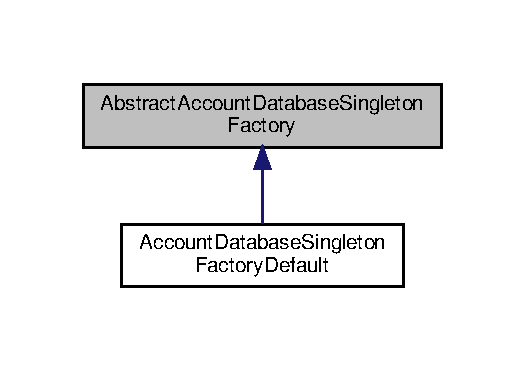
\includegraphics[width=252pt]{d7/d46/classAbstractAccountDatabaseSingletonFactory__inherit__graph}
\end{center}
\end{figure}
\subsection*{Public Member Functions}
\begin{DoxyCompactItemize}
\item 
\mbox{\Hypertarget{classAbstractAccountDatabaseSingletonFactory_a8e2cec9f578de9cc99d83a9a494e886a}\label{classAbstractAccountDatabaseSingletonFactory_a8e2cec9f578de9cc99d83a9a494e886a}} 
virtual \hyperlink{classInterfaceAccountDatabase}{Interface\+Account\+Database} \& {\bfseries get\+Instance} ()=0
\item 
\mbox{\Hypertarget{classAbstractAccountDatabaseSingletonFactory_a50aec839eeb5934d7de857a5ae4f9e49}\label{classAbstractAccountDatabaseSingletonFactory_a50aec839eeb5934d7de857a5ae4f9e49}} 
virtual \hyperlink{classAbstractAccountDatabaseSingletonFactory}{Abstract\+Account\+Database\+Singleton\+Factory} $\ast$ {\bfseries clone} () const
\end{DoxyCompactItemize}
\subsection*{Protected Member Functions}
\begin{DoxyCompactItemize}
\item 
\mbox{\Hypertarget{classAbstractAccountDatabaseSingletonFactory_a12bb4c8056a319fab670c1ea0508624a}\label{classAbstractAccountDatabaseSingletonFactory_a12bb4c8056a319fab670c1ea0508624a}} 
virtual \hyperlink{classAbstractAccountDatabaseSingletonFactory}{Abstract\+Account\+Database\+Singleton\+Factory} $\ast$ {\bfseries do\+Clone} () const =0
\end{DoxyCompactItemize}


\subsection{Detailed Description}
Abstract factory, which provide access to single global account database.  Abstract factory, which provide access to single global account database. 

The documentation for this class was generated from the following file\+:\begin{DoxyCompactItemize}
\item 
src/account/accountdatabase.\+h\end{DoxyCompactItemize}

\hypertarget{classAbstractFileTransmission}{}\section{Abstract\+File\+Transmission Class Reference}
\label{classAbstractFileTransmission}\index{Abstract\+File\+Transmission@{Abstract\+File\+Transmission}}


Abstract class for handle low-\/level transmission.  Abstract class for handle low-\/level transmission.  




{\ttfamily \#include $<$filetransmission.\+h$>$}



Inheritance diagram for Abstract\+File\+Transmission\+:\nopagebreak
\begin{figure}[H]
\begin{center}
\leavevmode
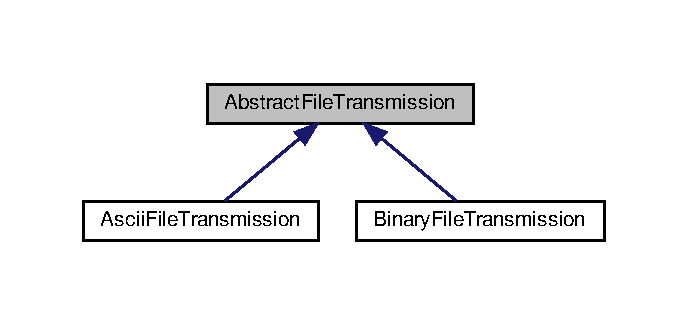
\includegraphics[width=330pt]{dc/d3d/classAbstractFileTransmission__inherit__graph}
\end{center}
\end{figure}
\subsection*{Data Structures}
\begin{DoxyCompactItemize}
\item 
struct \hyperlink{structAbstractFileTransmission_1_1FileTransmissionReceiveException}{File\+Transmission\+Receive\+Exception}
\item 
struct \hyperlink{structAbstractFileTransmission_1_1FileTransmissionSendException}{File\+Transmission\+Send\+Exception}
\end{DoxyCompactItemize}
\subsection*{Public Types}
\begin{DoxyCompactItemize}
\item 
\mbox{\Hypertarget{classAbstractFileTransmission_af504e5e76391ce4a4e5b8a090ba199b1}\label{classAbstractFileTransmission_af504e5e76391ce4a4e5b8a090ba199b1}} 
using {\bfseries Internal\+Buffer} = std\+::array$<$ char, B\+U\+F\+F\+\_\+\+S\+I\+ZE $>$
\item 
\mbox{\Hypertarget{classAbstractFileTransmission_a24ecd3592c22a52086a960772a8e08c1}\label{classAbstractFileTransmission_a24ecd3592c22a52086a960772a8e08c1}} 
using {\bfseries External\+Buffer} = std\+::array$<$ Q\+Char, B\+U\+F\+F\+\_\+\+S\+I\+ZE $>$
\end{DoxyCompactItemize}
\subsection*{Public Member Functions}
\begin{DoxyCompactItemize}
\item 
\hyperlink{classAbstractFileTransmission_a91b9eb10d6cf9fbaebf2c23c9cdeb81c}{Abstract\+File\+Transmission} (const \hyperlink{classInterfaceTransmissionReader}{Interface\+Transmission\+Reader} \&reader, const \hyperlink{classInterfaceTransmissionWriter}{Interface\+Transmission\+Writer} \&writer)
\item 
void \hyperlink{classAbstractFileTransmission_ad49bd97cf93532458f0eb2808af75e28}{send} (int data\+Channel\+Socket, const Q\+File \&file)
\item 
void \hyperlink{classAbstractFileTransmission_a0eaf52c2d4a568833867b59c01d0259b}{receive} (int data\+Channel\+Socket, const Q\+File \&file)
\end{DoxyCompactItemize}
\subsection*{Static Public Member Functions}
\begin{DoxyCompactItemize}
\item 
\mbox{\Hypertarget{classAbstractFileTransmission_a3c05e06b2b543e8ab5a0d0850eed5c6b}\label{classAbstractFileTransmission_a3c05e06b2b543e8ab5a0d0850eed5c6b}} 
static void {\bfseries set\+Bsd\+Socket\+Factory} (const \hyperlink{classInterfaceBsdSocketFactory}{Interface\+Bsd\+Socket\+Factory} \&new\+Factory)
\item 
\mbox{\Hypertarget{classAbstractFileTransmission_a7612e8c1f03dfdbd1f0e463b2935ba39}\label{classAbstractFileTransmission_a7612e8c1f03dfdbd1f0e463b2935ba39}} 
static size\+\_\+t {\bfseries get\+Buff\+Size} ()
\end{DoxyCompactItemize}


\subsection{Detailed Description}
Abstract class for handle low-\/level transmission.  Abstract class for handle low-\/level transmission. 

\subsection{Constructor \& Destructor Documentation}
\mbox{\Hypertarget{classAbstractFileTransmission_a91b9eb10d6cf9fbaebf2c23c9cdeb81c}\label{classAbstractFileTransmission_a91b9eb10d6cf9fbaebf2c23c9cdeb81c}} 
\index{Abstract\+File\+Transmission@{Abstract\+File\+Transmission}!Abstract\+File\+Transmission@{Abstract\+File\+Transmission}}
\index{Abstract\+File\+Transmission@{Abstract\+File\+Transmission}!Abstract\+File\+Transmission@{Abstract\+File\+Transmission}}
\subsubsection{\texorpdfstring{Abstract\+File\+Transmission()}{AbstractFileTransmission()}}
{\footnotesize\ttfamily Abstract\+File\+Transmission\+::\+Abstract\+File\+Transmission (\begin{DoxyParamCaption}\item[{const \hyperlink{classInterfaceTransmissionReader}{Interface\+Transmission\+Reader} \&}]{reader,  }\item[{const \hyperlink{classInterfaceTransmissionWriter}{Interface\+Transmission\+Writer} \&}]{writer }\end{DoxyParamCaption})}


\begin{DoxyParams}{Parameters}
{\em reader} & Interface to the transmission reader \\
\hline
{\em writer} & Interface to the transmission writer \\
\hline
\end{DoxyParams}


\subsection{Member Function Documentation}
\mbox{\Hypertarget{classAbstractFileTransmission_a0eaf52c2d4a568833867b59c01d0259b}\label{classAbstractFileTransmission_a0eaf52c2d4a568833867b59c01d0259b}} 
\index{Abstract\+File\+Transmission@{Abstract\+File\+Transmission}!receive@{receive}}
\index{receive@{receive}!Abstract\+File\+Transmission@{Abstract\+File\+Transmission}}
\subsubsection{\texorpdfstring{receive()}{receive()}}
{\footnotesize\ttfamily void Abstract\+File\+Transmission\+::receive (\begin{DoxyParamCaption}\item[{int}]{data\+Channel\+Socket,  }\item[{const Q\+File \&}]{file }\end{DoxyParamCaption})}


\begin{DoxyParams}{Parameters}
{\em data\+Channel\+Socket} & Socket to communication with client on data channel \\
\hline
{\em file} & File where received data will we written \\
\hline
\end{DoxyParams}
\mbox{\Hypertarget{classAbstractFileTransmission_ad49bd97cf93532458f0eb2808af75e28}\label{classAbstractFileTransmission_ad49bd97cf93532458f0eb2808af75e28}} 
\index{Abstract\+File\+Transmission@{Abstract\+File\+Transmission}!send@{send}}
\index{send@{send}!Abstract\+File\+Transmission@{Abstract\+File\+Transmission}}
\subsubsection{\texorpdfstring{send()}{send()}}
{\footnotesize\ttfamily void Abstract\+File\+Transmission\+::send (\begin{DoxyParamCaption}\item[{int}]{data\+Channel\+Socket,  }\item[{const Q\+File \&}]{file }\end{DoxyParamCaption})}


\begin{DoxyParams}{Parameters}
{\em data\+Channel\+Socket} & Socket to communication with client on data channel \\
\hline
{\em file} & File to be sent \\
\hline
\end{DoxyParams}


The documentation for this class was generated from the following files\+:\begin{DoxyCompactItemize}
\item 
src/transmission/filetransmission.\+h\item 
src/transmission/filetransmission.\+cpp\end{DoxyCompactItemize}

\hypertarget{classAbstractFTPcommand}{}\section{Abstract\+F\+T\+Pcommand Class Reference}
\label{classAbstractFTPcommand}\index{Abstract\+F\+T\+Pcommand@{Abstract\+F\+T\+Pcommand}}


Abstract class for ftp command.  Abstract class for ftp command.  




{\ttfamily \#include $<$ftpcommand.\+h$>$}



Inheritance diagram for Abstract\+F\+T\+Pcommand\+:\nopagebreak
\begin{figure}[H]
\begin{center}
\leavevmode
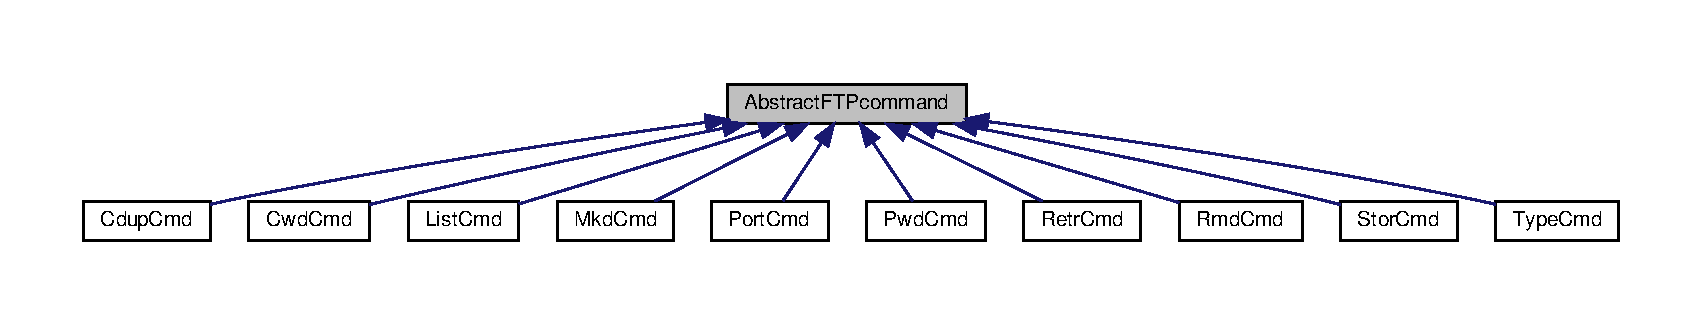
\includegraphics[width=350pt]{db/dab/classAbstractFTPcommand__inherit__graph}
\end{center}
\end{figure}
\subsection*{Public Member Functions}
\begin{DoxyCompactItemize}
\item 
\mbox{\Hypertarget{classAbstractFTPcommand_a11d459d4fda2bf6125706648d8e94a36}\label{classAbstractFTPcommand_a11d459d4fda2bf6125706648d8e94a36}} 
virtual void {\bfseries execute} ()=0
\end{DoxyCompactItemize}
\subsection*{Static Public Member Functions}
\begin{DoxyCompactItemize}
\item 
\mbox{\Hypertarget{classAbstractFTPcommand_a7d84c3fe6d23e3d73cee642957f8f45f}\label{classAbstractFTPcommand_a7d84c3fe6d23e3d73cee642957f8f45f}} 
static void {\bfseries set\+Account\+Database\+Factory} (const \hyperlink{classAbstractAccountDatabaseSingletonFactory}{Abstract\+Account\+Database\+Singleton\+Factory} \&new\+Factory)
\end{DoxyCompactItemize}
\subsection*{Protected Member Functions}
\begin{DoxyCompactItemize}
\item 
\hyperlink{classInterfaceAccountDatabase}{Interface\+Account\+Database} \& \hyperlink{classAbstractFTPcommand_a22bac678c35be37939d485fb866f759e}{get\+Database} () const
\end{DoxyCompactItemize}


\subsection{Detailed Description}
Abstract class for ftp command.  Abstract class for ftp command. 

\subsection{Member Function Documentation}
\mbox{\Hypertarget{classAbstractFTPcommand_a22bac678c35be37939d485fb866f759e}\label{classAbstractFTPcommand_a22bac678c35be37939d485fb866f759e}} 
\index{Abstract\+F\+T\+Pcommand@{Abstract\+F\+T\+Pcommand}!get\+Database@{get\+Database}}
\index{get\+Database@{get\+Database}!Abstract\+F\+T\+Pcommand@{Abstract\+F\+T\+Pcommand}}
\subsubsection{\texorpdfstring{get\+Database()}{getDatabase()}}
{\footnotesize\ttfamily \hyperlink{classInterfaceAccountDatabase}{Interface\+Account\+Database} \& Abstract\+F\+T\+Pcommand\+::get\+Database (\begin{DoxyParamCaption}{ }\end{DoxyParamCaption}) const\hspace{0.3cm}{\ttfamily [protected]}}

\begin{DoxyReturn}{Returns}
Default account database, or modified account database. 
\end{DoxyReturn}


The documentation for this class was generated from the following files\+:\begin{DoxyCompactItemize}
\item 
src/ftpcommand/ftpcommand.\+h\item 
src/ftpcommand/ftpcommand.\+cpp\end{DoxyCompactItemize}

\hypertarget{classAbstractFTPservice}{}\section{Abstract\+F\+T\+Pservice Class Reference}
\label{classAbstractFTPservice}\index{Abstract\+F\+T\+Pservice@{Abstract\+F\+T\+Pservice}}


Abstract ftp service class, provide low-\/level handle of command.  Abstract ftp service class, provide low-\/level handle of command.  




{\ttfamily \#include $<$F\+T\+Pservice.\+h$>$}



Inheritance diagram for Abstract\+F\+T\+Pservice\+:\nopagebreak
\begin{figure}[H]
\begin{center}
\leavevmode
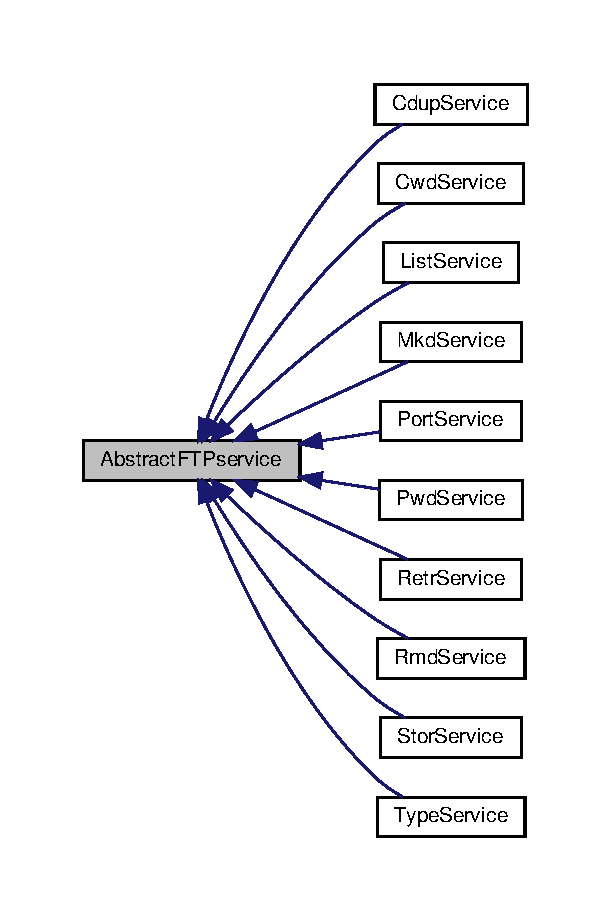
\includegraphics[width=293pt]{d2/d55/classAbstractFTPservice__inherit__graph}
\end{center}
\end{figure}
\subsection*{Public Types}
\begin{DoxyCompactItemize}
\item 
\mbox{\Hypertarget{classAbstractFTPservice_a9ded9b5067150f1d98ad0d40e489f5d3}\label{classAbstractFTPservice_a9ded9b5067150f1d98ad0d40e489f5d3}} 
using {\bfseries Exception\+Reply\+Code} = Q\+Map$<$ \hyperlink{classNamedException}{Named\+Exception}, \hyperlink{classReplyCode}{Reply\+Code} $\ast$ $>$
\end{DoxyCompactItemize}
\subsection*{Public Member Functions}
\begin{DoxyCompactItemize}
\item 
\mbox{\Hypertarget{classAbstractFTPservice_a82d0f243f0e89dfd07f40d5d42adbb13}\label{classAbstractFTPservice_a82d0f243f0e89dfd07f40d5d42adbb13}} 
void {\bfseries start} ()
\item 
Q\+String \hyperlink{classAbstractFTPservice_a48c4d339fde37882e48fc9e007184e2f}{reply\+Before} ()
\item 
Q\+String \hyperlink{classAbstractFTPservice_aa689acc6cb72ed5255a1ca407059be83}{reply\+After} ()
\end{DoxyCompactItemize}
\subsection*{Protected Member Functions}
\begin{DoxyCompactItemize}
\item 
\hyperlink{classAbstractFTPservice_acaddc197e13656887d4ee18f1119d755}{Abstract\+F\+T\+Pservice} (\hyperlink{classAbstractFTPcommand}{Abstract\+F\+T\+Pcommand} $\ast$const new\+Cmd)
\item 
\hyperlink{classAbstractFTPservice_ac420f6055d26efcd511d146a4e52155a}{Abstract\+F\+T\+Pservice} (\hyperlink{classAbstractFTPcommand}{Abstract\+F\+T\+Pcommand} $\ast$const new\+Cmd, Exception\+Reply\+Code new\+Reply\+Codes)
\item 
virtual Q\+String \hyperlink{classAbstractFTPservice_a3ac6c2518376864615d68199845d910a}{parse\+Reply\+Before} (\hyperlink{classAbstractFTPcommand}{Abstract\+F\+T\+Pcommand} $\ast$const)
\begin{DoxyCompactList}\small\item\em Allow to redefined default reply after ending command. \end{DoxyCompactList}\item 
virtual Q\+String \hyperlink{classAbstractFTPservice_a914cd7810f9e8e563dd0dd7bb34d4224}{parse\+Reply\+After} (\hyperlink{classAbstractFTPcommand}{Abstract\+F\+T\+Pcommand} $\ast$const)
\begin{DoxyCompactList}\small\item\em Allow to redefined default reply after ending command. \end{DoxyCompactList}\end{DoxyCompactItemize}


\subsection{Detailed Description}
Abstract ftp service class, provide low-\/level handle of command.  Abstract ftp service class, provide low-\/level handle of command. 

\subsection{Constructor \& Destructor Documentation}
\mbox{\Hypertarget{classAbstractFTPservice_acaddc197e13656887d4ee18f1119d755}\label{classAbstractFTPservice_acaddc197e13656887d4ee18f1119d755}} 
\index{Abstract\+F\+T\+Pservice@{Abstract\+F\+T\+Pservice}!Abstract\+F\+T\+Pservice@{Abstract\+F\+T\+Pservice}}
\index{Abstract\+F\+T\+Pservice@{Abstract\+F\+T\+Pservice}!Abstract\+F\+T\+Pservice@{Abstract\+F\+T\+Pservice}}
\subsubsection{\texorpdfstring{Abstract\+F\+T\+Pservice()}{AbstractFTPservice()}\hspace{0.1cm}{\footnotesize\ttfamily [1/2]}}
{\footnotesize\ttfamily Abstract\+F\+T\+Pservice\+::\+Abstract\+F\+T\+Pservice (\begin{DoxyParamCaption}\item[{\hyperlink{classAbstractFTPcommand}{Abstract\+F\+T\+Pcommand} $\ast$const}]{new\+Cmd }\end{DoxyParamCaption})\hspace{0.3cm}{\ttfamily [protected]}}


\begin{DoxyParams}{Parameters}
{\em new\+Cmd} & Command to handle. \\
\hline
\end{DoxyParams}
\mbox{\Hypertarget{classAbstractFTPservice_ac420f6055d26efcd511d146a4e52155a}\label{classAbstractFTPservice_ac420f6055d26efcd511d146a4e52155a}} 
\index{Abstract\+F\+T\+Pservice@{Abstract\+F\+T\+Pservice}!Abstract\+F\+T\+Pservice@{Abstract\+F\+T\+Pservice}}
\index{Abstract\+F\+T\+Pservice@{Abstract\+F\+T\+Pservice}!Abstract\+F\+T\+Pservice@{Abstract\+F\+T\+Pservice}}
\subsubsection{\texorpdfstring{Abstract\+F\+T\+Pservice()}{AbstractFTPservice()}\hspace{0.1cm}{\footnotesize\ttfamily [2/2]}}
{\footnotesize\ttfamily Abstract\+F\+T\+Pservice\+::\+Abstract\+F\+T\+Pservice (\begin{DoxyParamCaption}\item[{\hyperlink{classAbstractFTPcommand}{Abstract\+F\+T\+Pcommand} $\ast$const}]{new\+Cmd,  }\item[{Abstract\+F\+T\+Pservice\+::\+Exception\+Reply\+Code}]{new\+Reply\+Codes }\end{DoxyParamCaption})\hspace{0.3cm}{\ttfamily [protected]}}


\begin{DoxyParams}{Parameters}
{\em new\+Cmd} & Command to handle. \\
\hline
{\em new\+Reply\+Codes} & Exceptions that may be throw by command and replies assigned to them. \\
\hline
\end{DoxyParams}


\subsection{Member Function Documentation}
\mbox{\Hypertarget{classAbstractFTPservice_a914cd7810f9e8e563dd0dd7bb34d4224}\label{classAbstractFTPservice_a914cd7810f9e8e563dd0dd7bb34d4224}} 
\index{Abstract\+F\+T\+Pservice@{Abstract\+F\+T\+Pservice}!parse\+Reply\+After@{parse\+Reply\+After}}
\index{parse\+Reply\+After@{parse\+Reply\+After}!Abstract\+F\+T\+Pservice@{Abstract\+F\+T\+Pservice}}
\subsubsection{\texorpdfstring{parse\+Reply\+After()}{parseReplyAfter()}}
{\footnotesize\ttfamily Q\+String Abstract\+F\+T\+Pservice\+::parse\+Reply\+After (\begin{DoxyParamCaption}\item[{\hyperlink{classAbstractFTPcommand}{Abstract\+F\+T\+Pcommand} $\ast$ const}]{ }\end{DoxyParamCaption})\hspace{0.3cm}{\ttfamily [protected]}, {\ttfamily [virtual]}}



Allow to redefined default reply after ending command. 

Default reply is empty string. \begin{DoxyReturn}{Returns}
Reply after ending command. 
\end{DoxyReturn}
\mbox{\Hypertarget{classAbstractFTPservice_a3ac6c2518376864615d68199845d910a}\label{classAbstractFTPservice_a3ac6c2518376864615d68199845d910a}} 
\index{Abstract\+F\+T\+Pservice@{Abstract\+F\+T\+Pservice}!parse\+Reply\+Before@{parse\+Reply\+Before}}
\index{parse\+Reply\+Before@{parse\+Reply\+Before}!Abstract\+F\+T\+Pservice@{Abstract\+F\+T\+Pservice}}
\subsubsection{\texorpdfstring{parse\+Reply\+Before()}{parseReplyBefore()}}
{\footnotesize\ttfamily Q\+String Abstract\+F\+T\+Pservice\+::parse\+Reply\+Before (\begin{DoxyParamCaption}\item[{\hyperlink{classAbstractFTPcommand}{Abstract\+F\+T\+Pcommand} $\ast$ const}]{ }\end{DoxyParamCaption})\hspace{0.3cm}{\ttfamily [protected]}, {\ttfamily [virtual]}}



Allow to redefined default reply after ending command. 

Default reply is code number 200. \begin{DoxyReturn}{Returns}
Reply before starting command. 
\end{DoxyReturn}
\mbox{\Hypertarget{classAbstractFTPservice_aa689acc6cb72ed5255a1ca407059be83}\label{classAbstractFTPservice_aa689acc6cb72ed5255a1ca407059be83}} 
\index{Abstract\+F\+T\+Pservice@{Abstract\+F\+T\+Pservice}!reply\+After@{reply\+After}}
\index{reply\+After@{reply\+After}!Abstract\+F\+T\+Pservice@{Abstract\+F\+T\+Pservice}}
\subsubsection{\texorpdfstring{reply\+After()}{replyAfter()}}
{\footnotesize\ttfamily Q\+String Abstract\+F\+T\+Pservice\+::reply\+After (\begin{DoxyParamCaption}{ }\end{DoxyParamCaption})}

\begin{DoxyReturn}{Returns}
Reply after ending command. 
\end{DoxyReturn}
\mbox{\Hypertarget{classAbstractFTPservice_a48c4d339fde37882e48fc9e007184e2f}\label{classAbstractFTPservice_a48c4d339fde37882e48fc9e007184e2f}} 
\index{Abstract\+F\+T\+Pservice@{Abstract\+F\+T\+Pservice}!reply\+Before@{reply\+Before}}
\index{reply\+Before@{reply\+Before}!Abstract\+F\+T\+Pservice@{Abstract\+F\+T\+Pservice}}
\subsubsection{\texorpdfstring{reply\+Before()}{replyBefore()}}
{\footnotesize\ttfamily Q\+String Abstract\+F\+T\+Pservice\+::reply\+Before (\begin{DoxyParamCaption}{ }\end{DoxyParamCaption})}

\begin{DoxyReturn}{Returns}
Reply before starting command. 
\end{DoxyReturn}


The documentation for this class was generated from the following files\+:\begin{DoxyCompactItemize}
\item 
src/controller/services/F\+T\+Pservice.\+h\item 
src/controller/services/F\+T\+Pservice.\+cpp\end{DoxyCompactItemize}

\hypertarget{classAccountDatabaseDefault}{}\section{Account\+Database\+Default Class Reference}
\label{classAccountDatabaseDefault}\index{Account\+Database\+Default@{Account\+Database\+Default}}


Default implementation of account database interface.  




{\ttfamily \#include $<$accountdatabase.\+h$>$}



Inheritance diagram for Account\+Database\+Default\+:\nopagebreak
\begin{figure}[H]
\begin{center}
\leavevmode
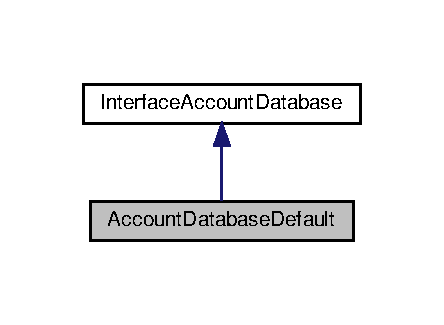
\includegraphics[width=213pt]{d7/d4b/classAccountDatabaseDefault__inherit__graph}
\end{center}
\end{figure}


Collaboration diagram for Account\+Database\+Default\+:\nopagebreak
\begin{figure}[H]
\begin{center}
\leavevmode
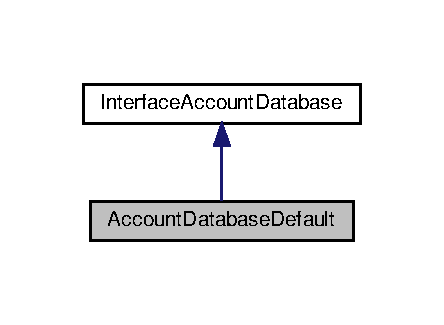
\includegraphics[width=213pt]{df/dcc/classAccountDatabaseDefault__coll__graph}
\end{center}
\end{figure}
\subsection*{Public Member Functions}
\begin{DoxyCompactItemize}
\item 
\mbox{\Hypertarget{classAccountDatabaseDefault_a1ec811d4b91f7a50173d4febd4b288df}\label{classAccountDatabaseDefault_a1ec811d4b91f7a50173d4febd4b288df}} 
void {\bfseries add\+Account\+Info} (const \hyperlink{classAccountInfo}{Account\+Info} \&account\+Info) override
\item 
\mbox{\Hypertarget{classAccountDatabaseDefault_a2f927b06f1794578d5f4fe919dd8f760}\label{classAccountDatabaseDefault_a2f927b06f1794578d5f4fe919dd8f760}} 
\hyperlink{classAccountInfo}{Account\+Info} {\bfseries get\+Account\+Info} (int command\+Channel\+Socket) override
\item 
\mbox{\Hypertarget{classAccountDatabaseDefault_a272c8d7c00deffd4823245ae4843e1e6}\label{classAccountDatabaseDefault_a272c8d7c00deffd4823245ae4843e1e6}} 
void {\bfseries set\+Account\+Info} (const \hyperlink{classAccountInfo}{Account\+Info} \&account\+Info) override
\item 
\mbox{\Hypertarget{classAccountDatabaseDefault_a0e3f47244d8cc41d976ebc53bb4910a7}\label{classAccountDatabaseDefault_a0e3f47244d8cc41d976ebc53bb4910a7}} 
void {\bfseries del\+Account\+Info} (int command\+Channel\+Socket) override
\item 
\mbox{\Hypertarget{classAccountDatabaseDefault_af4bac6718adab77d641035bbfadb981b}\label{classAccountDatabaseDefault_af4bac6718adab77d641035bbfadb981b}} 
void {\bfseries reset\+Database} () override
\end{DoxyCompactItemize}


\subsection{Detailed Description}
Default implementation of account database interface. 

The documentation for this class was generated from the following files\+:\begin{DoxyCompactItemize}
\item 
src/account/accountdatabase.\+h\item 
src/account/accountdatabase.\+cpp\end{DoxyCompactItemize}

\hypertarget{classAccountDatabaseSingletonFactoryDefault}{}\section{Account\+Database\+Singleton\+Factory\+Default Class Reference}
\label{classAccountDatabaseSingletonFactoryDefault}\index{Account\+Database\+Singleton\+Factory\+Default@{Account\+Database\+Singleton\+Factory\+Default}}


Default implementation of abstract account database singleton factory.  




{\ttfamily \#include $<$accountdatabase.\+h$>$}



Inheritance diagram for Account\+Database\+Singleton\+Factory\+Default\+:\nopagebreak
\begin{figure}[H]
\begin{center}
\leavevmode
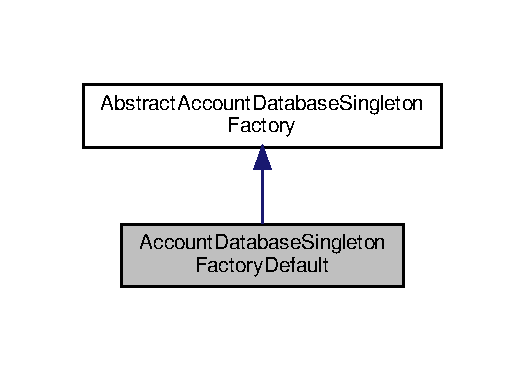
\includegraphics[width=252pt]{d3/d4d/classAccountDatabaseSingletonFactoryDefault__inherit__graph}
\end{center}
\end{figure}


Collaboration diagram for Account\+Database\+Singleton\+Factory\+Default\+:\nopagebreak
\begin{figure}[H]
\begin{center}
\leavevmode
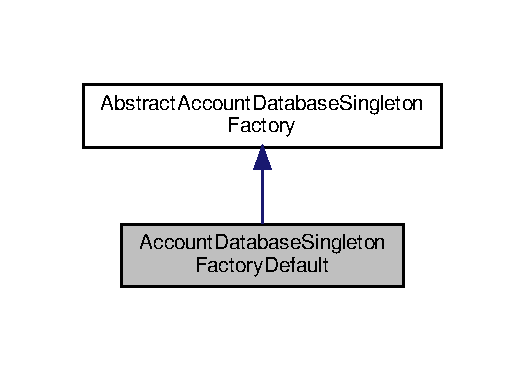
\includegraphics[width=252pt]{db/d2c/classAccountDatabaseSingletonFactoryDefault__coll__graph}
\end{center}
\end{figure}
\subsection*{Public Member Functions}
\begin{DoxyCompactItemize}
\item 
\mbox{\Hypertarget{classAccountDatabaseSingletonFactoryDefault_a4087f03d6d173982d0a681c828bb0f27}\label{classAccountDatabaseSingletonFactoryDefault_a4087f03d6d173982d0a681c828bb0f27}} 
virtual \hyperlink{classInterfaceAccountDatabase}{Interface\+Account\+Database} \& {\bfseries get\+Instance} () override
\item 
\mbox{\Hypertarget{classAccountDatabaseSingletonFactoryDefault_afc11e06d193ebc6792551a51496c5b35}\label{classAccountDatabaseSingletonFactoryDefault_afc11e06d193ebc6792551a51496c5b35}} 
virtual \hyperlink{classAbstractAccountDatabaseSingletonFactory}{Abstract\+Account\+Database\+Singleton\+Factory} $\ast$ {\bfseries do\+Clone} () const override
\end{DoxyCompactItemize}
\subsection*{Additional Inherited Members}


\subsection{Detailed Description}
Default implementation of abstract account database singleton factory. 

The documentation for this class was generated from the following files\+:\begin{DoxyCompactItemize}
\item 
src/account/accountdatabase.\+h\item 
src/account/accountdatabase.\+cpp\end{DoxyCompactItemize}

\hypertarget{structInterfaceAccountDatabase_1_1AccountExistsException}{}\section{Interface\+Account\+Database\+:\+:Account\+Exists\+Exception Struct Reference}
\label{structInterfaceAccountDatabase_1_1AccountExistsException}\index{Interface\+Account\+Database\+::\+Account\+Exists\+Exception@{Interface\+Account\+Database\+::\+Account\+Exists\+Exception}}


Inheritance diagram for Interface\+Account\+Database\+:\+:Account\+Exists\+Exception\+:\nopagebreak
\begin{figure}[H]
\begin{center}
\leavevmode
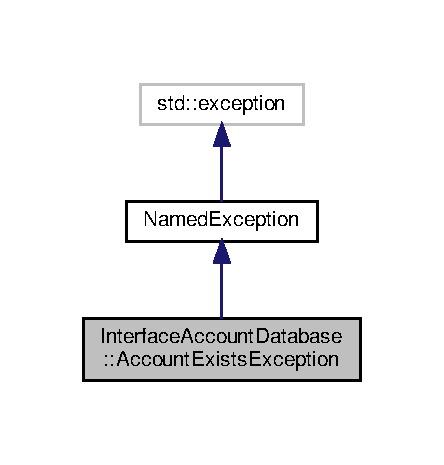
\includegraphics[width=213pt]{d2/d3f/structInterfaceAccountDatabase_1_1AccountExistsException__inherit__graph}
\end{center}
\end{figure}


Collaboration diagram for Interface\+Account\+Database\+:\+:Account\+Exists\+Exception\+:\nopagebreak
\begin{figure}[H]
\begin{center}
\leavevmode
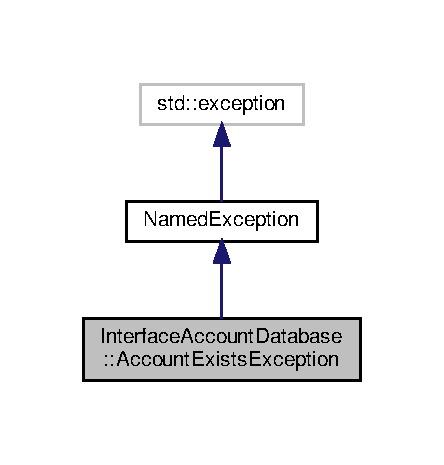
\includegraphics[width=213pt]{d1/d39/structInterfaceAccountDatabase_1_1AccountExistsException__coll__graph}
\end{center}
\end{figure}
\subsection*{Public Member Functions}
\begin{DoxyCompactItemize}
\item 
\mbox{\Hypertarget{structInterfaceAccountDatabase_1_1AccountExistsException_a0ef320378d8fca372095b5251717434b}\label{structInterfaceAccountDatabase_1_1AccountExistsException_a0ef320378d8fca372095b5251717434b}} 
virtual const char $\ast$ {\bfseries what} () const noexcept override
\item 
\mbox{\Hypertarget{structInterfaceAccountDatabase_1_1AccountExistsException_a24b1fb2147c44dabf801eb30087137d7}\label{structInterfaceAccountDatabase_1_1AccountExistsException_a24b1fb2147c44dabf801eb30087137d7}} 
virtual Q\+String {\bfseries name} () override
\end{DoxyCompactItemize}


The documentation for this struct was generated from the following file\+:\begin{DoxyCompactItemize}
\item 
src/account/accountdatabase.\+h\end{DoxyCompactItemize}

\hypertarget{classAccountInfo}{}\section{Account\+Info Class Reference}
\label{classAccountInfo}\index{Account\+Info@{Account\+Info}}


Structure for handle ftp user information.  




{\ttfamily \#include $<$accountinfo.\+h$>$}

\subsection*{Public Types}
\begin{DoxyCompactItemize}
\item 
\mbox{\Hypertarget{classAccountInfo_a7c804c71299c02010e99514eafb04a63}\label{classAccountInfo_a7c804c71299c02010e99514eafb04a63}} 
enum {\bfseries Transmission\+Type} \{ {\bfseries Ascii}, 
{\bfseries Binary}
 \}
\end{DoxyCompactItemize}
\subsection*{Public Member Functions}
\begin{DoxyCompactItemize}
\item 
\mbox{\Hypertarget{classAccountInfo_afc6cb2f3521a7ebf8d16f004f61533f4}\label{classAccountInfo_afc6cb2f3521a7ebf8d16f004f61533f4}} 
sockaddr\+\_\+in {\bfseries get\+Command\+Channel\+Address} () const
\item 
\mbox{\Hypertarget{classAccountInfo_a473dfbf8850784ad41454d5e2086d172}\label{classAccountInfo_a473dfbf8850784ad41454d5e2086d172}} 
void {\bfseries set\+Command\+Channel\+Address} (const sockaddr\+\_\+in \&value)
\item 
\mbox{\Hypertarget{classAccountInfo_af22c3388b12cd7f0073921d8416561a5}\label{classAccountInfo_af22c3388b12cd7f0073921d8416561a5}} 
sockaddr\+\_\+in {\bfseries get\+Data\+Channel\+Address} () const
\item 
\mbox{\Hypertarget{classAccountInfo_a744ad5f4281ab1c2719c95554fcefd14}\label{classAccountInfo_a744ad5f4281ab1c2719c95554fcefd14}} 
void {\bfseries set\+Data\+Channel\+Address} (const sockaddr\+\_\+in \&value)
\item 
\mbox{\Hypertarget{classAccountInfo_a646c0cf60d1817fbc0308527908f2eb0}\label{classAccountInfo_a646c0cf60d1817fbc0308527908f2eb0}} 
int {\bfseries get\+Command\+Channel\+Socket} () const
\item 
\mbox{\Hypertarget{classAccountInfo_a8f26940fe646a532c98aec6ada6ee113}\label{classAccountInfo_a8f26940fe646a532c98aec6ada6ee113}} 
void {\bfseries set\+Command\+Channel\+Socket} (int value)
\item 
\mbox{\Hypertarget{classAccountInfo_ace3df4d708b419f64a6593d80bed5f32}\label{classAccountInfo_ace3df4d708b419f64a6593d80bed5f32}} 
Transmission\+Type {\bfseries get\+Transmission\+Type} () const
\item 
\mbox{\Hypertarget{classAccountInfo_a49608ec2fcbae0ff6a984fa6667808ce}\label{classAccountInfo_a49608ec2fcbae0ff6a984fa6667808ce}} 
void {\bfseries set\+Transmission\+Type} (const Transmission\+Type \&value)
\item 
\mbox{\Hypertarget{classAccountInfo_a268caf5cf743d60cfa4381de959d926a}\label{classAccountInfo_a268caf5cf743d60cfa4381de959d926a}} 
\hyperlink{classInterfaceFTPfileSystem}{Interface\+F\+T\+Pfile\+System} $\ast$ {\bfseries get\+File\+System} () const
\end{DoxyCompactItemize}
\subsection*{Static Public Member Functions}
\begin{DoxyCompactItemize}
\item 
\mbox{\Hypertarget{classAccountInfo_aa3c9fcca47dc666090d8a316b2fe72d2}\label{classAccountInfo_aa3c9fcca47dc666090d8a316b2fe72d2}} 
static Q\+File\+Info {\bfseries get\+Default\+Root\+Path} ()
\item 
\mbox{\Hypertarget{classAccountInfo_a3a88b32d15964447cedf68513c0ec006}\label{classAccountInfo_a3a88b32d15964447cedf68513c0ec006}} 
static void \hyperlink{classAccountInfo_a3a88b32d15964447cedf68513c0ec006}{set\+Default\+Root\+Path} (const Q\+File\+Info \&value)
\begin{DoxyCompactList}\small\item\em Have to be done before server is running. \end{DoxyCompactList}\end{DoxyCompactItemize}


\subsection{Detailed Description}
Structure for handle ftp user information. 

The documentation for this class was generated from the following files\+:\begin{DoxyCompactItemize}
\item 
src/account/accountinfo.\+h\item 
src/account/accountinfo.\+cpp\end{DoxyCompactItemize}

\hypertarget{structInterfaceAccountDatabase_1_1AccountNotFoundException}{}\section{Interface\+Account\+Database\+:\+:Account\+Not\+Found\+Exception Struct Reference}
\label{structInterfaceAccountDatabase_1_1AccountNotFoundException}\index{Interface\+Account\+Database\+::\+Account\+Not\+Found\+Exception@{Interface\+Account\+Database\+::\+Account\+Not\+Found\+Exception}}


Inheritance diagram for Interface\+Account\+Database\+:\+:Account\+Not\+Found\+Exception\+:\nopagebreak
\begin{figure}[H]
\begin{center}
\leavevmode
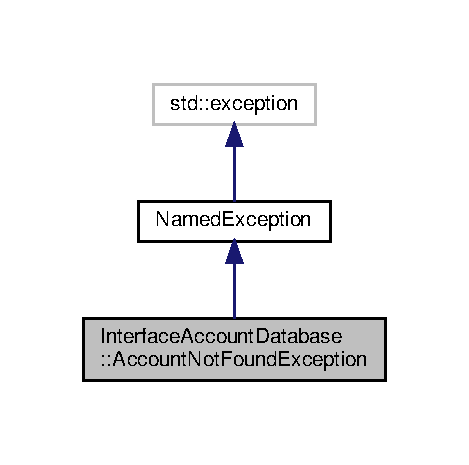
\includegraphics[width=225pt]{da/def/structInterfaceAccountDatabase_1_1AccountNotFoundException__inherit__graph}
\end{center}
\end{figure}


Collaboration diagram for Interface\+Account\+Database\+:\+:Account\+Not\+Found\+Exception\+:\nopagebreak
\begin{figure}[H]
\begin{center}
\leavevmode
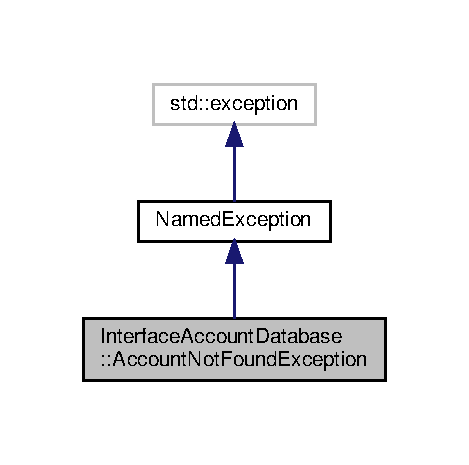
\includegraphics[width=225pt]{d1/daa/structInterfaceAccountDatabase_1_1AccountNotFoundException__coll__graph}
\end{center}
\end{figure}
\subsection*{Public Member Functions}
\begin{DoxyCompactItemize}
\item 
\mbox{\Hypertarget{structInterfaceAccountDatabase_1_1AccountNotFoundException_a6283365bf82ec589999a2e88bf2b8b6d}\label{structInterfaceAccountDatabase_1_1AccountNotFoundException_a6283365bf82ec589999a2e88bf2b8b6d}} 
virtual const char $\ast$ {\bfseries what} () const noexcept override
\item 
\mbox{\Hypertarget{structInterfaceAccountDatabase_1_1AccountNotFoundException_aa2d09d087a5cc970426c128b03eb92bd}\label{structInterfaceAccountDatabase_1_1AccountNotFoundException_aa2d09d087a5cc970426c128b03eb92bd}} 
virtual Q\+String {\bfseries name} () override
\end{DoxyCompactItemize}


The documentation for this struct was generated from the following file\+:\begin{DoxyCompactItemize}
\item 
src/account/accountdatabase.\+h\end{DoxyCompactItemize}

\hypertarget{classAsciiFileTransmission}{}\section{Ascii\+File\+Transmission Class Reference}
\label{classAsciiFileTransmission}\index{Ascii\+File\+Transmission@{Ascii\+File\+Transmission}}


Send or receive file through data channel in A\+S\+C\+II chars.  




{\ttfamily \#include $<$asciifiletransmission.\+h$>$}



Inheritance diagram for Ascii\+File\+Transmission\+:\nopagebreak
\begin{figure}[H]
\begin{center}
\leavevmode
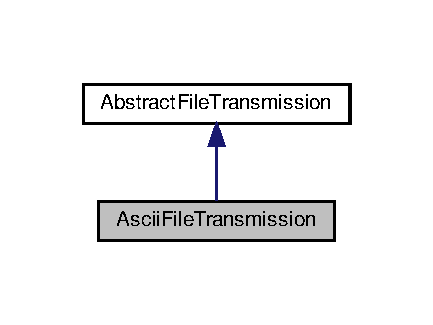
\includegraphics[width=208pt]{d8/d5c/classAsciiFileTransmission__inherit__graph}
\end{center}
\end{figure}


Collaboration diagram for Ascii\+File\+Transmission\+:\nopagebreak
\begin{figure}[H]
\begin{center}
\leavevmode
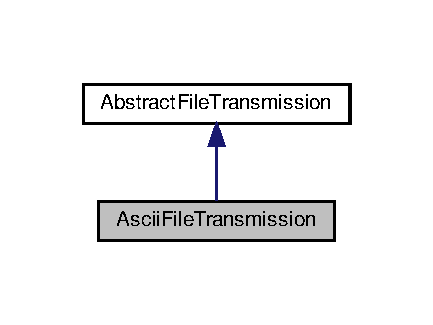
\includegraphics[width=208pt]{d9/dfb/classAsciiFileTransmission__coll__graph}
\end{center}
\end{figure}
\subsection*{Additional Inherited Members}


\subsection{Detailed Description}
Send or receive file through data channel in A\+S\+C\+II chars. 

The documentation for this class was generated from the following files\+:\begin{DoxyCompactItemize}
\item 
src/transmission/types/asciifiletransmission.\+h\item 
src/transmission/types/asciifiletransmission.\+cpp\end{DoxyCompactItemize}

\hypertarget{classAsciiTransmissionReader}{}\section{Ascii\+Transmission\+Reader Class Reference}
\label{classAsciiTransmissionReader}\index{Ascii\+Transmission\+Reader@{Ascii\+Transmission\+Reader}}


Inheritance diagram for Ascii\+Transmission\+Reader\+:
\nopagebreak
\begin{figure}[H]
\begin{center}
\leavevmode
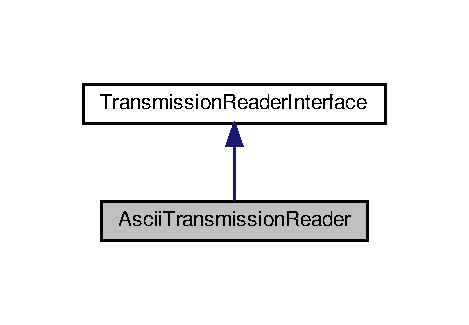
\includegraphics[width=225pt]{classAsciiTransmissionReader__inherit__graph}
\end{center}
\end{figure}


Collaboration diagram for Ascii\+Transmission\+Reader\+:
\nopagebreak
\begin{figure}[H]
\begin{center}
\leavevmode
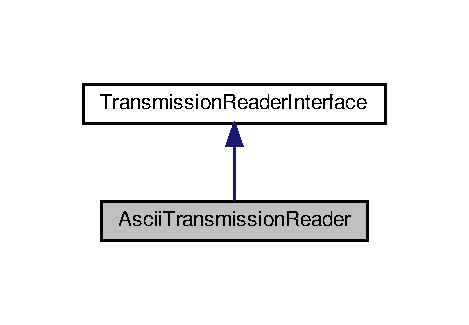
\includegraphics[width=225pt]{classAsciiTransmissionReader__coll__graph}
\end{center}
\end{figure}
\subsection*{Additional Inherited Members}


The documentation for this class was generated from the following files\+:\begin{DoxyCompactItemize}
\item 
src/transmission/types/asciitransmission.\+h\item 
src/transmission/types/asciitransmission.\+cpp\end{DoxyCompactItemize}

\hypertarget{classAsciiTransmissionWriter}{}\section{Ascii\+Transmission\+Writer Class Reference}
\label{classAsciiTransmissionWriter}\index{Ascii\+Transmission\+Writer@{Ascii\+Transmission\+Writer}}


Inheritance diagram for Ascii\+Transmission\+Writer\+:
\nopagebreak
\begin{figure}[H]
\begin{center}
\leavevmode
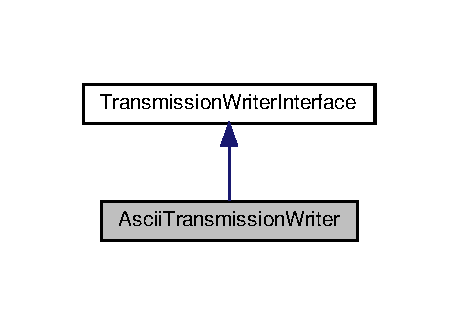
\includegraphics[width=220pt]{classAsciiTransmissionWriter__inherit__graph}
\end{center}
\end{figure}


Collaboration diagram for Ascii\+Transmission\+Writer\+:
\nopagebreak
\begin{figure}[H]
\begin{center}
\leavevmode
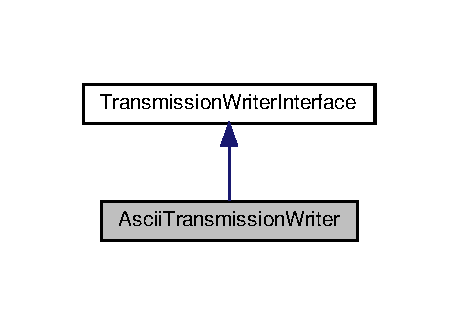
\includegraphics[width=220pt]{classAsciiTransmissionWriter__coll__graph}
\end{center}
\end{figure}
\subsection*{Additional Inherited Members}


The documentation for this class was generated from the following files\+:\begin{DoxyCompactItemize}
\item 
src/transmission/types/asciitransmission.\+h\item 
src/transmission/types/asciitransmission.\+cpp\end{DoxyCompactItemize}

\hypertarget{classBinaryFileTransmission}{}\section{Binary\+File\+Transmission Class Reference}
\label{classBinaryFileTransmission}\index{Binary\+File\+Transmission@{Binary\+File\+Transmission}}


Send or receive file through data channel in binary chars.  




{\ttfamily \#include $<$binaryfiletransmission.\+h$>$}



Inheritance diagram for Binary\+File\+Transmission\+:\nopagebreak
\begin{figure}[H]
\begin{center}
\leavevmode
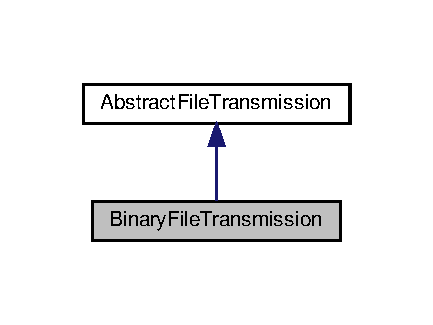
\includegraphics[width=208pt]{d0/d38/classBinaryFileTransmission__inherit__graph}
\end{center}
\end{figure}


Collaboration diagram for Binary\+File\+Transmission\+:\nopagebreak
\begin{figure}[H]
\begin{center}
\leavevmode
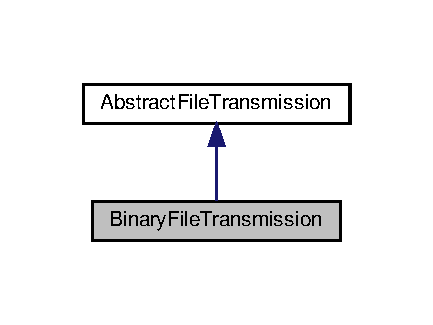
\includegraphics[width=208pt]{da/d1d/classBinaryFileTransmission__coll__graph}
\end{center}
\end{figure}
\subsection*{Additional Inherited Members}


\subsection{Detailed Description}
Send or receive file through data channel in binary chars. 

The documentation for this class was generated from the following files\+:\begin{DoxyCompactItemize}
\item 
src/transmission/types/binaryfiletransmission.\+h\item 
src/transmission/types/binaryfiletransmission.\+cpp\end{DoxyCompactItemize}

\hypertarget{classBinaryTransmissionReader}{}\section{Binary\+Transmission\+Reader Class Reference}
\label{classBinaryTransmissionReader}\index{Binary\+Transmission\+Reader@{Binary\+Transmission\+Reader}}


Read file in binary chars.  




{\ttfamily \#include $<$binaryfiletransmission.\+h$>$}



Inheritance diagram for Binary\+Transmission\+Reader\+:\nopagebreak
\begin{figure}[H]
\begin{center}
\leavevmode
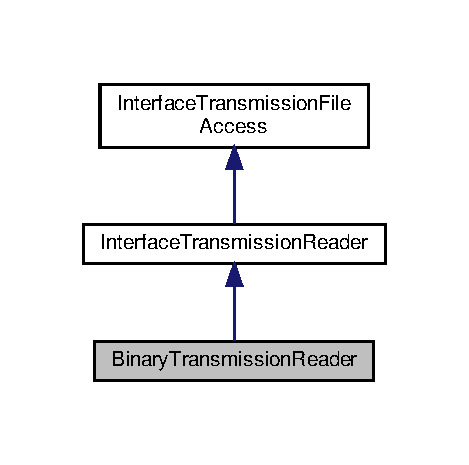
\includegraphics[width=225pt]{d4/dda/classBinaryTransmissionReader__inherit__graph}
\end{center}
\end{figure}


Collaboration diagram for Binary\+Transmission\+Reader\+:\nopagebreak
\begin{figure}[H]
\begin{center}
\leavevmode
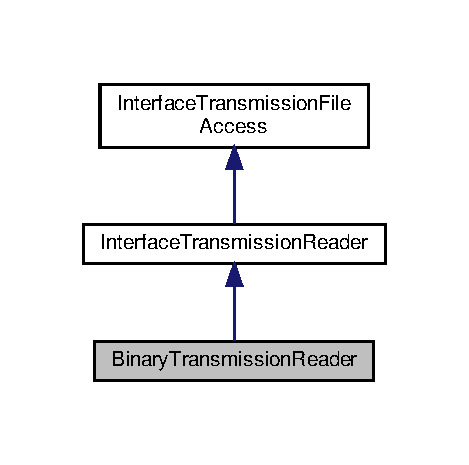
\includegraphics[width=225pt]{d5/da5/classBinaryTransmissionReader__coll__graph}
\end{center}
\end{figure}
\subsection*{Public Member Functions}
\begin{DoxyCompactItemize}
\item 
virtual void \hyperlink{classBinaryTransmissionReader_a28c85fe81913ccb4ba6aee44d84dbf7d}{init} (const Q\+File \&file) override
\begin{DoxyCompactList}\small\item\em Open file. \end{DoxyCompactList}\item 
virtual Buffer\+Info \hyperlink{classBinaryTransmissionReader_a003a0b7a500a15ddfc573e6f54006b0c}{read\+Data\+Portion} () override
\begin{DoxyCompactList}\small\item\em Read data from the file and write them to the buffer. \end{DoxyCompactList}\item 
\mbox{\Hypertarget{classBinaryTransmissionReader_af324c2292bcc28c64d11d754c110e9bf}\label{classBinaryTransmissionReader_af324c2292bcc28c64d11d754c110e9bf}} 
virtual bool {\bfseries is\+End\+Of\+File} () override
\item 
\mbox{\Hypertarget{classBinaryTransmissionReader_add9c1a4adb7fe8098d81bb0f5f916c93}\label{classBinaryTransmissionReader_add9c1a4adb7fe8098d81bb0f5f916c93}} 
virtual void \hyperlink{classBinaryTransmissionReader_add9c1a4adb7fe8098d81bb0f5f916c93}{clean\+Up} () override
\begin{DoxyCompactList}\small\item\em Close file. \end{DoxyCompactList}\end{DoxyCompactItemize}
\subsection*{Additional Inherited Members}


\subsection{Detailed Description}
Read file in binary chars. 

\subsection{Member Function Documentation}
\mbox{\Hypertarget{classBinaryTransmissionReader_a28c85fe81913ccb4ba6aee44d84dbf7d}\label{classBinaryTransmissionReader_a28c85fe81913ccb4ba6aee44d84dbf7d}} 
\index{Binary\+Transmission\+Reader@{Binary\+Transmission\+Reader}!init@{init}}
\index{init@{init}!Binary\+Transmission\+Reader@{Binary\+Transmission\+Reader}}
\subsubsection{\texorpdfstring{init()}{init()}}
{\footnotesize\ttfamily void Binary\+Transmission\+Reader\+::init (\begin{DoxyParamCaption}\item[{const Q\+File \&}]{file }\end{DoxyParamCaption})\hspace{0.3cm}{\ttfamily [override]}, {\ttfamily [virtual]}}



Open file. 


\begin{DoxyParams}{Parameters}
{\em file} & File to be read/write \\
\hline
\end{DoxyParams}


Implements \hyperlink{classInterfaceTransmissionFileAccess_a8c423ccb527b1dda62c798a75b6eb690}{Interface\+Transmission\+File\+Access}.

\mbox{\Hypertarget{classBinaryTransmissionReader_a003a0b7a500a15ddfc573e6f54006b0c}\label{classBinaryTransmissionReader_a003a0b7a500a15ddfc573e6f54006b0c}} 
\index{Binary\+Transmission\+Reader@{Binary\+Transmission\+Reader}!read\+Data\+Portion@{read\+Data\+Portion}}
\index{read\+Data\+Portion@{read\+Data\+Portion}!Binary\+Transmission\+Reader@{Binary\+Transmission\+Reader}}
\subsubsection{\texorpdfstring{read\+Data\+Portion()}{readDataPortion()}}
{\footnotesize\ttfamily Interface\+Transmission\+File\+Access\+::\+Buffer\+Info Binary\+Transmission\+Reader\+::read\+Data\+Portion (\begin{DoxyParamCaption}{ }\end{DoxyParamCaption})\hspace{0.3cm}{\ttfamily [override]}, {\ttfamily [virtual]}}



Read data from the file and write them to the buffer. 

\begin{DoxyReturn}{Returns}
Buffer with data size. 
\end{DoxyReturn}


Implements \hyperlink{classInterfaceTransmissionReader_ab8733fbc3a4f6dc8279c363212fd3f51}{Interface\+Transmission\+Reader}.



The documentation for this class was generated from the following files\+:\begin{DoxyCompactItemize}
\item 
src/transmission/types/binaryfiletransmission.\+h\item 
src/transmission/types/binaryfiletransmission.\+cpp\end{DoxyCompactItemize}

\hypertarget{classBinaryTransmissionWriter}{}\section{Binary\+Transmission\+Writer Class Reference}
\label{classBinaryTransmissionWriter}\index{Binary\+Transmission\+Writer@{Binary\+Transmission\+Writer}}


Write to file binary chars.  




{\ttfamily \#include $<$binaryfiletransmission.\+h$>$}



Inheritance diagram for Binary\+Transmission\+Writer\+:\nopagebreak
\begin{figure}[H]
\begin{center}
\leavevmode
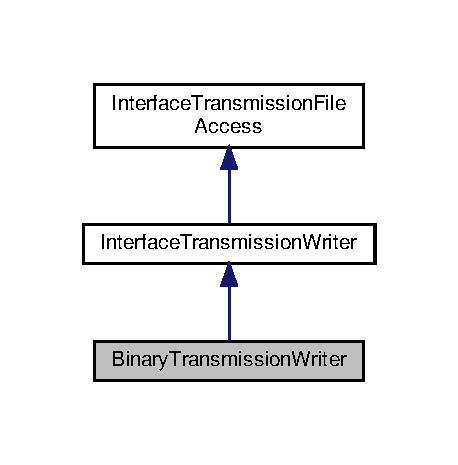
\includegraphics[width=220pt]{d4/d45/classBinaryTransmissionWriter__inherit__graph}
\end{center}
\end{figure}


Collaboration diagram for Binary\+Transmission\+Writer\+:\nopagebreak
\begin{figure}[H]
\begin{center}
\leavevmode
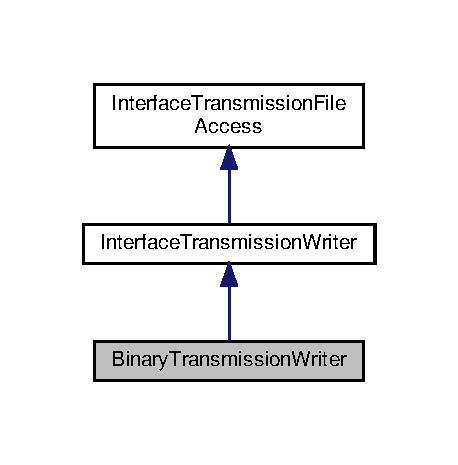
\includegraphics[width=220pt]{da/d75/classBinaryTransmissionWriter__coll__graph}
\end{center}
\end{figure}
\subsection*{Public Member Functions}
\begin{DoxyCompactItemize}
\item 
virtual void \hyperlink{classBinaryTransmissionWriter_a40cc3d88d6501af5db2ed2acd05caacc}{init} (const Q\+File \&file) override
\begin{DoxyCompactList}\small\item\em Open file. \end{DoxyCompactList}\item 
virtual void \hyperlink{classBinaryTransmissionWriter_aaeee88a165c1a53ef89849c08df6a5e1}{write\+Data\+Portion} (Buffer\+Info buffer) override
\begin{DoxyCompactList}\small\item\em Read data from the buffer and write them to the file. \end{DoxyCompactList}\item 
\mbox{\Hypertarget{classBinaryTransmissionWriter_ad30e89ab71e1317464fedc4671f2da86}\label{classBinaryTransmissionWriter_ad30e89ab71e1317464fedc4671f2da86}} 
virtual void \hyperlink{classBinaryTransmissionWriter_ad30e89ab71e1317464fedc4671f2da86}{clean\+Up} () override
\begin{DoxyCompactList}\small\item\em Close file. \end{DoxyCompactList}\end{DoxyCompactItemize}
\subsection*{Additional Inherited Members}


\subsection{Detailed Description}
Write to file binary chars. 

\subsection{Member Function Documentation}
\mbox{\Hypertarget{classBinaryTransmissionWriter_a40cc3d88d6501af5db2ed2acd05caacc}\label{classBinaryTransmissionWriter_a40cc3d88d6501af5db2ed2acd05caacc}} 
\index{Binary\+Transmission\+Writer@{Binary\+Transmission\+Writer}!init@{init}}
\index{init@{init}!Binary\+Transmission\+Writer@{Binary\+Transmission\+Writer}}
\subsubsection{\texorpdfstring{init()}{init()}}
{\footnotesize\ttfamily void Binary\+Transmission\+Writer\+::init (\begin{DoxyParamCaption}\item[{const Q\+File \&}]{file }\end{DoxyParamCaption})\hspace{0.3cm}{\ttfamily [override]}, {\ttfamily [virtual]}}



Open file. 


\begin{DoxyParams}{Parameters}
{\em file} & File to be read/write \\
\hline
\end{DoxyParams}


Implements \hyperlink{classInterfaceTransmissionFileAccess_a8c423ccb527b1dda62c798a75b6eb690}{Interface\+Transmission\+File\+Access}.

\mbox{\Hypertarget{classBinaryTransmissionWriter_aaeee88a165c1a53ef89849c08df6a5e1}\label{classBinaryTransmissionWriter_aaeee88a165c1a53ef89849c08df6a5e1}} 
\index{Binary\+Transmission\+Writer@{Binary\+Transmission\+Writer}!write\+Data\+Portion@{write\+Data\+Portion}}
\index{write\+Data\+Portion@{write\+Data\+Portion}!Binary\+Transmission\+Writer@{Binary\+Transmission\+Writer}}
\subsubsection{\texorpdfstring{write\+Data\+Portion()}{writeDataPortion()}}
{\footnotesize\ttfamily void Binary\+Transmission\+Writer\+::write\+Data\+Portion (\begin{DoxyParamCaption}\item[{Buffer\+Info}]{info }\end{DoxyParamCaption})\hspace{0.3cm}{\ttfamily [override]}, {\ttfamily [virtual]}}



Read data from the buffer and write them to the file. 


\begin{DoxyParams}{Parameters}
{\em info} & Buffer with data size. \\
\hline
\end{DoxyParams}


Implements \hyperlink{classInterfaceTransmissionWriter_a024c3a22d937e659259f2eb242b3ea97}{Interface\+Transmission\+Writer}.



The documentation for this class was generated from the following files\+:\begin{DoxyCompactItemize}
\item 
src/transmission/types/binaryfiletransmission.\+h\item 
src/transmission/types/binaryfiletransmission.\+cpp\end{DoxyCompactItemize}

\hypertarget{classBsdSocketFactoryDefault}{}\section{Bsd\+Socket\+Factory\+Default Class Reference}
\label{classBsdSocketFactoryDefault}\index{Bsd\+Socket\+Factory\+Default@{Bsd\+Socket\+Factory\+Default}}


Default implementation of bsd socket factory interface.  




{\ttfamily \#include $<$bsdsocketfactory.\+h$>$}



Inheritance diagram for Bsd\+Socket\+Factory\+Default\+:\nopagebreak
\begin{figure}[H]
\begin{center}
\leavevmode
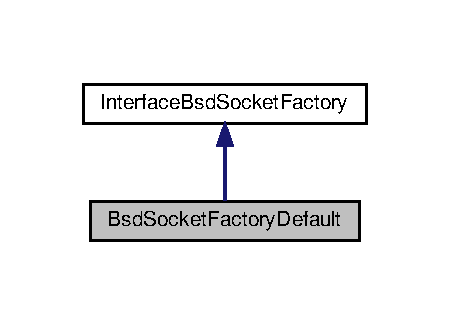
\includegraphics[width=216pt]{dd/da7/classBsdSocketFactoryDefault__inherit__graph}
\end{center}
\end{figure}


Collaboration diagram for Bsd\+Socket\+Factory\+Default\+:\nopagebreak
\begin{figure}[H]
\begin{center}
\leavevmode
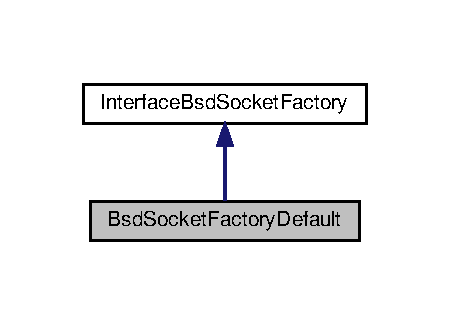
\includegraphics[width=216pt]{d5/d23/classBsdSocketFactoryDefault__coll__graph}
\end{center}
\end{figure}
\subsection*{Public Member Functions}
\begin{DoxyCompactItemize}
\item 
\mbox{\Hypertarget{classBsdSocketFactoryDefault_ae56c8979788fa1092ee7f8b3ed52d2ba}\label{classBsdSocketFactoryDefault_ae56c8979788fa1092ee7f8b3ed52d2ba}} 
virtual int {\bfseries socket} (int \+\_\+\+\_\+domain, int \+\_\+\+\_\+type, int \+\_\+\+\_\+protocol) override
\item 
\mbox{\Hypertarget{classBsdSocketFactoryDefault_a1e2faa4b38f70b662d5fcff501cd1dd1}\label{classBsdSocketFactoryDefault_a1e2faa4b38f70b662d5fcff501cd1dd1}} 
virtual int {\bfseries connect} (int \+\_\+\+\_\+fd, \+\_\+\+\_\+\+C\+O\+N\+S\+T\+\_\+\+S\+O\+C\+K\+A\+D\+D\+R\+\_\+\+A\+RG \+\_\+\+\_\+addr, socklen\+\_\+t \+\_\+\+\_\+len) override
\item 
\mbox{\Hypertarget{classBsdSocketFactoryDefault_a83eaa1d6e746a676ffa049b284fa7d0a}\label{classBsdSocketFactoryDefault_a83eaa1d6e746a676ffa049b284fa7d0a}} 
virtual ssize\+\_\+t {\bfseries write} (int \+\_\+\+\_\+fd, const void $\ast$\+\_\+\+\_\+buf, size\+\_\+t \+\_\+\+\_\+n) override
\item 
\mbox{\Hypertarget{classBsdSocketFactoryDefault_a17cb735df563f8e9d8329f2293f96209}\label{classBsdSocketFactoryDefault_a17cb735df563f8e9d8329f2293f96209}} 
virtual ssize\+\_\+t {\bfseries read} (int \+\_\+\+\_\+fd, void $\ast$\+\_\+\+\_\+buf, size\+\_\+t \+\_\+\+\_\+nbytes) override
\item 
\mbox{\Hypertarget{classBsdSocketFactoryDefault_ab601ea872ecf968e63b1ced7bde5e0da}\label{classBsdSocketFactoryDefault_ab601ea872ecf968e63b1ced7bde5e0da}} 
virtual int {\bfseries bind} (int \+\_\+\+\_\+fd, \+\_\+\+\_\+\+C\+O\+N\+S\+T\+\_\+\+S\+O\+C\+K\+A\+D\+D\+R\+\_\+\+A\+RG \+\_\+\+\_\+addr, socklen\+\_\+t \+\_\+\+\_\+len) override
\item 
\mbox{\Hypertarget{classBsdSocketFactoryDefault_a60acd85e3aa1439b3e91ee673d358ad7}\label{classBsdSocketFactoryDefault_a60acd85e3aa1439b3e91ee673d358ad7}} 
virtual int {\bfseries listen} (int \+\_\+\+\_\+fd, int \+\_\+\+\_\+n) override
\item 
\mbox{\Hypertarget{classBsdSocketFactoryDefault_a4cd3062f5fe9a8fcc0191e51ab2e021a}\label{classBsdSocketFactoryDefault_a4cd3062f5fe9a8fcc0191e51ab2e021a}} 
virtual int {\bfseries accept} (int \+\_\+\+\_\+fd, \+\_\+\+\_\+\+S\+O\+C\+K\+A\+D\+D\+R\+\_\+\+A\+RG \+\_\+\+\_\+addr, socklen\+\_\+t $\ast$\+\_\+\+\_\+restrict \+\_\+\+\_\+addr\+\_\+len) override
\item 
\mbox{\Hypertarget{classBsdSocketFactoryDefault_a74d05cce49a7760d8469f43f731f9a3d}\label{classBsdSocketFactoryDefault_a74d05cce49a7760d8469f43f731f9a3d}} 
virtual int {\bfseries close} (int \+\_\+\+\_\+fd) override
\item 
\mbox{\Hypertarget{classBsdSocketFactoryDefault_a92c76d39e336ac82954f869268df68a4}\label{classBsdSocketFactoryDefault_a92c76d39e336ac82954f869268df68a4}} 
virtual int {\bfseries getsockopt} (int \+\_\+\+\_\+fd, int \+\_\+\+\_\+level, int \+\_\+\+\_\+optname, void $\ast$\+\_\+\+\_\+restrict \+\_\+\+\_\+optval, socklen\+\_\+t $\ast$\+\_\+\+\_\+restrict \+\_\+\+\_\+optlen) override
\item 
\mbox{\Hypertarget{classBsdSocketFactoryDefault_af92759f0383e9314f889482bd5b65e63}\label{classBsdSocketFactoryDefault_af92759f0383e9314f889482bd5b65e63}} 
virtual \hyperlink{classInterfaceBsdSocketFactory}{Interface\+Bsd\+Socket\+Factory} $\ast$ {\bfseries do\+Clone} () const override
\end{DoxyCompactItemize}
\subsection*{Additional Inherited Members}


\subsection{Detailed Description}
Default implementation of bsd socket factory interface. 

The documentation for this class was generated from the following files\+:\begin{DoxyCompactItemize}
\item 
src/bsdsocket/bsdsocketfactory.\+h\item 
src/bsdsocket/bsdsocketfactory.\+cpp\end{DoxyCompactItemize}

\hypertarget{classCdupCmd}{}\section{Cdup\+Cmd Class Reference}
\label{classCdupCmd}\index{Cdup\+Cmd@{Cdup\+Cmd}}


Change working directory to parent.  




{\ttfamily \#include $<$cdupcmd.\+h$>$}



Inheritance diagram for Cdup\+Cmd\+:\nopagebreak
\begin{figure}[H]
\begin{center}
\leavevmode
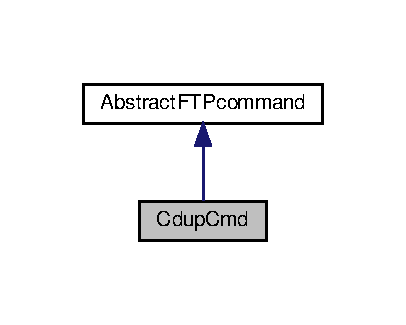
\includegraphics[width=195pt]{de/dbd/classCdupCmd__inherit__graph}
\end{center}
\end{figure}


Collaboration diagram for Cdup\+Cmd\+:\nopagebreak
\begin{figure}[H]
\begin{center}
\leavevmode
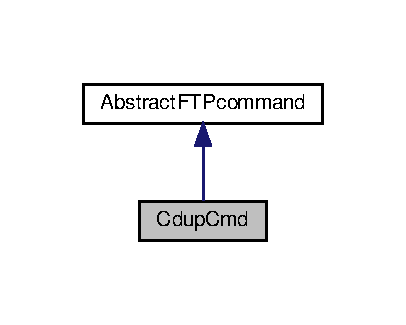
\includegraphics[width=195pt]{d3/dc6/classCdupCmd__coll__graph}
\end{center}
\end{figure}
\subsection*{Public Member Functions}
\begin{DoxyCompactItemize}
\item 
\hyperlink{classCdupCmd_aeb8d70fa7fd7a90dcf1571a50f829b41}{Cdup\+Cmd} (int command\+Channel\+Socket)
\item 
\mbox{\Hypertarget{classCdupCmd_a84e58f19f01e92852f2dbb4849065059}\label{classCdupCmd_a84e58f19f01e92852f2dbb4849065059}} 
void {\bfseries execute} () override
\end{DoxyCompactItemize}
\subsection*{Additional Inherited Members}


\subsection{Detailed Description}
Change working directory to parent. 

\subsection{Constructor \& Destructor Documentation}
\mbox{\Hypertarget{classCdupCmd_aeb8d70fa7fd7a90dcf1571a50f829b41}\label{classCdupCmd_aeb8d70fa7fd7a90dcf1571a50f829b41}} 
\index{Cdup\+Cmd@{Cdup\+Cmd}!Cdup\+Cmd@{Cdup\+Cmd}}
\index{Cdup\+Cmd@{Cdup\+Cmd}!Cdup\+Cmd@{Cdup\+Cmd}}
\subsubsection{\texorpdfstring{Cdup\+Cmd()}{CdupCmd()}}
{\footnotesize\ttfamily Cdup\+Cmd\+::\+Cdup\+Cmd (\begin{DoxyParamCaption}\item[{int}]{command\+Channel\+Socket }\end{DoxyParamCaption})}


\begin{DoxyParams}{Parameters}
{\em command\+Channel\+Socket} & Socket to communication with client on command channel \\
\hline
\end{DoxyParams}


The documentation for this class was generated from the following files\+:\begin{DoxyCompactItemize}
\item 
src/ftpcommand/cmds/cdupcmd.\+h\item 
src/ftpcommand/cmds/cdupcmd.\+cpp\end{DoxyCompactItemize}

\hypertarget{classCdupParser}{}\section{Cdup\+Parser Class Reference}
\label{classCdupParser}\index{Cdup\+Parser@{Cdup\+Parser}}


Parse C\+D\+UP ftp command.  




{\ttfamily \#include $<$cdupparser.\+h$>$}



Inheritance diagram for Cdup\+Parser\+:\nopagebreak
\begin{figure}[H]
\begin{center}
\leavevmode
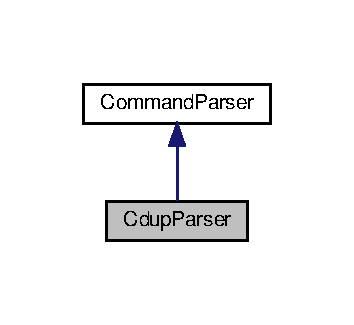
\includegraphics[width=170pt]{db/d72/classCdupParser__inherit__graph}
\end{center}
\end{figure}


Collaboration diagram for Cdup\+Parser\+:\nopagebreak
\begin{figure}[H]
\begin{center}
\leavevmode
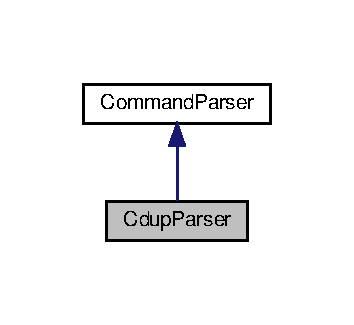
\includegraphics[width=170pt]{df/de4/classCdupParser__coll__graph}
\end{center}
\end{figure}
\subsection*{Public Member Functions}
\begin{DoxyCompactItemize}
\item 
virtual bool \hyperlink{classCdupParser_abfd60eab9d76c34867434b8a36289701}{parse} (const Q\+String \&input) override
\end{DoxyCompactItemize}


\subsection{Detailed Description}
Parse C\+D\+UP ftp command. 

\subsection{Member Function Documentation}
\mbox{\Hypertarget{classCdupParser_abfd60eab9d76c34867434b8a36289701}\label{classCdupParser_abfd60eab9d76c34867434b8a36289701}} 
\index{Cdup\+Parser@{Cdup\+Parser}!parse@{parse}}
\index{parse@{parse}!Cdup\+Parser@{Cdup\+Parser}}
\subsubsection{\texorpdfstring{parse()}{parse()}}
{\footnotesize\ttfamily bool Cdup\+Parser\+::parse (\begin{DoxyParamCaption}\item[{const Q\+String \&}]{input }\end{DoxyParamCaption})\hspace{0.3cm}{\ttfamily [override]}, {\ttfamily [virtual]}}

\begin{DoxyReturn}{Returns}
True if parse done successfuly 
\end{DoxyReturn}


Implements \hyperlink{classCommandParser_a5ed0855947a9b4500329f29b8123f2ea}{Command\+Parser}.



The documentation for this class was generated from the following files\+:\begin{DoxyCompactItemize}
\item 
src/ftpcommand/parsers/cdupparser.\+h\item 
src/ftpcommand/parsers/cdupparser.\+cpp\end{DoxyCompactItemize}

\hypertarget{classCdupService}{}\section{Cdup\+Service Class Reference}
\label{classCdupService}\index{Cdup\+Service@{Cdup\+Service}}


Service for handling C\+D\+UP ftp command.  




{\ttfamily \#include $<$cdupservice.\+h$>$}



Inheritance diagram for Cdup\+Service\+:\nopagebreak
\begin{figure}[H]
\begin{center}
\leavevmode
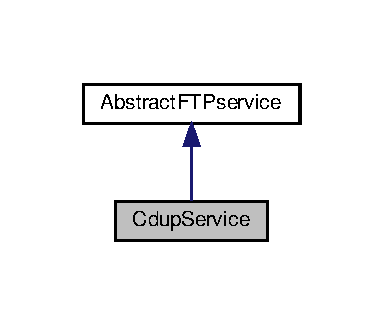
\includegraphics[width=184pt]{d3/d34/classCdupService__inherit__graph}
\end{center}
\end{figure}


Collaboration diagram for Cdup\+Service\+:\nopagebreak
\begin{figure}[H]
\begin{center}
\leavevmode
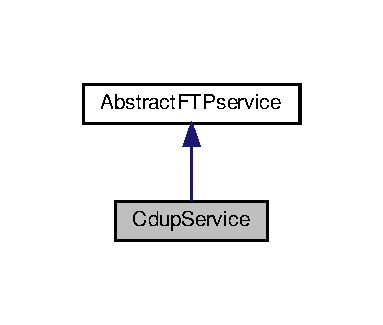
\includegraphics[width=184pt]{d6/d7f/classCdupService__coll__graph}
\end{center}
\end{figure}
\subsection*{Public Member Functions}
\begin{DoxyCompactItemize}
\item 
\hyperlink{classCdupService_ae8c9f05507b10e66af7f73a8cdf3236b}{Cdup\+Service} (int command\+Channel\+Socket)
\end{DoxyCompactItemize}
\subsection*{Additional Inherited Members}


\subsection{Detailed Description}
Service for handling C\+D\+UP ftp command. 

\subsection{Constructor \& Destructor Documentation}
\mbox{\Hypertarget{classCdupService_ae8c9f05507b10e66af7f73a8cdf3236b}\label{classCdupService_ae8c9f05507b10e66af7f73a8cdf3236b}} 
\index{Cdup\+Service@{Cdup\+Service}!Cdup\+Service@{Cdup\+Service}}
\index{Cdup\+Service@{Cdup\+Service}!Cdup\+Service@{Cdup\+Service}}
\subsubsection{\texorpdfstring{Cdup\+Service()}{CdupService()}}
{\footnotesize\ttfamily Cdup\+Service\+::\+Cdup\+Service (\begin{DoxyParamCaption}\item[{int}]{command\+Channel\+Socket }\end{DoxyParamCaption})}


\begin{DoxyParams}{Parameters}
{\em command\+Channel\+Socket} & Socket to communication with client on command channel \\
\hline
\end{DoxyParams}


The documentation for this class was generated from the following files\+:\begin{DoxyCompactItemize}
\item 
src/controller/services/srv/cdupservice.\+h\item 
src/controller/services/srv/cdupservice.\+cpp\end{DoxyCompactItemize}

\hypertarget{classCommandParser}{}\section{Command\+Parser Class Reference}
\label{classCommandParser}\index{Command\+Parser@{Command\+Parser}}


Inheritance diagram for Command\+Parser\+:\nopagebreak
\begin{figure}[H]
\begin{center}
\leavevmode
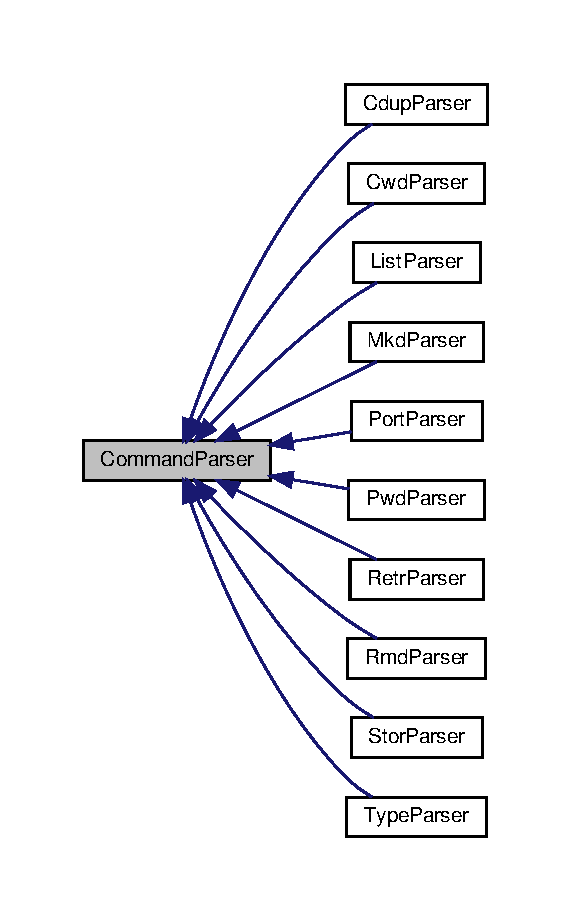
\includegraphics[width=274pt]{dc/d9e/classCommandParser__inherit__graph}
\end{center}
\end{figure}
\subsection*{Public Member Functions}
\begin{DoxyCompactItemize}
\item 
virtual bool \hyperlink{classCommandParser_a5ed0855947a9b4500329f29b8123f2ea}{parse} (const Q\+String \&input)=0
\end{DoxyCompactItemize}


\subsection{Member Function Documentation}
\mbox{\Hypertarget{classCommandParser_a5ed0855947a9b4500329f29b8123f2ea}\label{classCommandParser_a5ed0855947a9b4500329f29b8123f2ea}} 
\index{Command\+Parser@{Command\+Parser}!parse@{parse}}
\index{parse@{parse}!Command\+Parser@{Command\+Parser}}
\subsubsection{\texorpdfstring{parse()}{parse()}}
{\footnotesize\ttfamily virtual bool Command\+Parser\+::parse (\begin{DoxyParamCaption}\item[{const Q\+String \&}]{input }\end{DoxyParamCaption})\hspace{0.3cm}{\ttfamily [pure virtual]}}

\begin{DoxyReturn}{Returns}
True if parse done successfuly 
\end{DoxyReturn}


Implemented in \hyperlink{classPortParser_a7dbb8e4f695ed023c502a4c1f689d061}{Port\+Parser}, \hyperlink{classTypeParser_afc5fc9fbf55f8ecec885312dd396a353}{Type\+Parser}, \hyperlink{classCwdParser_a4037186e2a7229bc7499f138a559d47b}{Cwd\+Parser}, \hyperlink{classListParser_ad26061c7101e88d72fc86ccec6cc13a6}{List\+Parser}, \hyperlink{classMkdParser_ad886e57eeff70f08b2e057879fb0d9df}{Mkd\+Parser}, \hyperlink{classRetrParser_ace04fa9e7c638452de2d40dacc5a0471}{Retr\+Parser}, \hyperlink{classRmdParser_a19bc9f3a082934c2e8eb9eb8d8aee5f3}{Rmd\+Parser}, \hyperlink{classStorParser_a3b268c187eaf7135971fb553e9d10cf3}{Stor\+Parser}, \hyperlink{classCdupParser_abfd60eab9d76c34867434b8a36289701}{Cdup\+Parser}, and \hyperlink{classPwdParser_a2eb9149ae412e0d3a1b4b8f70f037224}{Pwd\+Parser}.



The documentation for this class was generated from the following file\+:\begin{DoxyCompactItemize}
\item 
src/ftpcommand/commandparser.\+h\end{DoxyCompactItemize}

\hypertarget{classCwdCmd}{}\section{Cwd\+Cmd Class Reference}
\label{classCwdCmd}\index{Cwd\+Cmd@{Cwd\+Cmd}}


Change working directory.  




{\ttfamily \#include $<$cwdcmd.\+h$>$}



Inheritance diagram for Cwd\+Cmd\+:\nopagebreak
\begin{figure}[H]
\begin{center}
\leavevmode
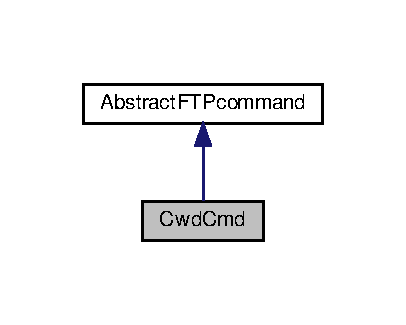
\includegraphics[width=195pt]{df/d02/classCwdCmd__inherit__graph}
\end{center}
\end{figure}


Collaboration diagram for Cwd\+Cmd\+:\nopagebreak
\begin{figure}[H]
\begin{center}
\leavevmode
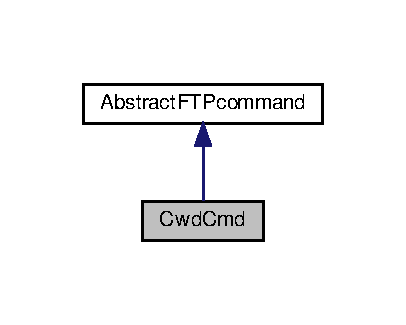
\includegraphics[width=195pt]{de/dbf/classCwdCmd__coll__graph}
\end{center}
\end{figure}
\subsection*{Public Member Functions}
\begin{DoxyCompactItemize}
\item 
\hyperlink{classCwdCmd_a625256040d74b4fec013d3a17119dc21}{Cwd\+Cmd} (int command\+Channel\+Socket, const Q\+String \&path)
\item 
\mbox{\Hypertarget{classCwdCmd_a39189ee40036d7f44290973787dc06e1}\label{classCwdCmd_a39189ee40036d7f44290973787dc06e1}} 
void {\bfseries execute} () override
\end{DoxyCompactItemize}
\subsection*{Additional Inherited Members}


\subsection{Detailed Description}
Change working directory. 

\subsection{Constructor \& Destructor Documentation}
\mbox{\Hypertarget{classCwdCmd_a625256040d74b4fec013d3a17119dc21}\label{classCwdCmd_a625256040d74b4fec013d3a17119dc21}} 
\index{Cwd\+Cmd@{Cwd\+Cmd}!Cwd\+Cmd@{Cwd\+Cmd}}
\index{Cwd\+Cmd@{Cwd\+Cmd}!Cwd\+Cmd@{Cwd\+Cmd}}
\subsubsection{\texorpdfstring{Cwd\+Cmd()}{CwdCmd()}}
{\footnotesize\ttfamily Cwd\+Cmd\+::\+Cwd\+Cmd (\begin{DoxyParamCaption}\item[{int}]{command\+Channel\+Socket,  }\item[{const Q\+String \&}]{path }\end{DoxyParamCaption})}


\begin{DoxyParams}{Parameters}
{\em command\+Channel\+Socket} & Socket to communication with client on command channel \\
\hline
{\em path} & New path \\
\hline
\end{DoxyParams}


The documentation for this class was generated from the following files\+:\begin{DoxyCompactItemize}
\item 
src/ftpcommand/cmds/cwdcmd.\+h\item 
src/ftpcommand/cmds/cwdcmd.\+cpp\end{DoxyCompactItemize}

\hypertarget{classCwdParser}{}\section{Cwd\+Parser Class Reference}
\label{classCwdParser}\index{Cwd\+Parser@{Cwd\+Parser}}


Parse C\+WD ftp command.  




{\ttfamily \#include $<$cwdparser.\+h$>$}



Inheritance diagram for Cwd\+Parser\+:\nopagebreak
\begin{figure}[H]
\begin{center}
\leavevmode
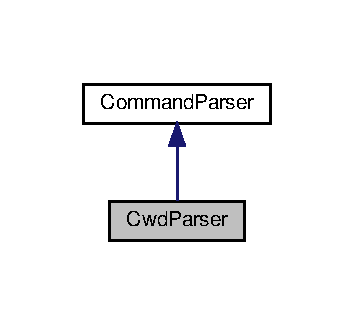
\includegraphics[width=170pt]{dc/d0e/classCwdParser__inherit__graph}
\end{center}
\end{figure}


Collaboration diagram for Cwd\+Parser\+:\nopagebreak
\begin{figure}[H]
\begin{center}
\leavevmode
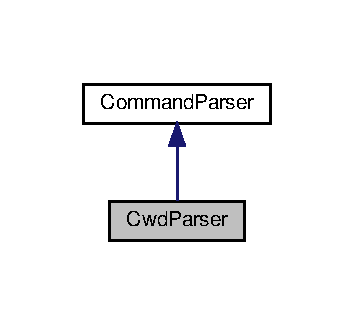
\includegraphics[width=170pt]{dc/dc7/classCwdParser__coll__graph}
\end{center}
\end{figure}
\subsection*{Public Member Functions}
\begin{DoxyCompactItemize}
\item 
virtual bool \hyperlink{classCwdParser_a4037186e2a7229bc7499f138a559d47b}{parse} (const Q\+String \&input) override
\item 
\mbox{\Hypertarget{classCwdParser_acfd6d9d6ec74418cb3176144541d3c6a}\label{classCwdParser_acfd6d9d6ec74418cb3176144541d3c6a}} 
Q\+String {\bfseries get\+Path} () const
\end{DoxyCompactItemize}


\subsection{Detailed Description}
Parse C\+WD ftp command. 

\subsection{Member Function Documentation}
\mbox{\Hypertarget{classCwdParser_a4037186e2a7229bc7499f138a559d47b}\label{classCwdParser_a4037186e2a7229bc7499f138a559d47b}} 
\index{Cwd\+Parser@{Cwd\+Parser}!parse@{parse}}
\index{parse@{parse}!Cwd\+Parser@{Cwd\+Parser}}
\subsubsection{\texorpdfstring{parse()}{parse()}}
{\footnotesize\ttfamily bool Cwd\+Parser\+::parse (\begin{DoxyParamCaption}\item[{const Q\+String \&}]{input }\end{DoxyParamCaption})\hspace{0.3cm}{\ttfamily [override]}, {\ttfamily [virtual]}}

\begin{DoxyReturn}{Returns}
True if parse done successfuly 
\end{DoxyReturn}


Implements \hyperlink{classCommandParser_a5ed0855947a9b4500329f29b8123f2ea}{Command\+Parser}.



The documentation for this class was generated from the following files\+:\begin{DoxyCompactItemize}
\item 
src/ftpcommand/parsers/cwdparser.\+h\item 
src/ftpcommand/parsers/cwdparser.\+cpp\end{DoxyCompactItemize}

\hypertarget{classCwdService}{}\section{Cwd\+Service Class Reference}
\label{classCwdService}\index{Cwd\+Service@{Cwd\+Service}}


Service for handling C\+WD ftp command.  




{\ttfamily \#include $<$cwdservice.\+h$>$}



Inheritance diagram for Cwd\+Service\+:\nopagebreak
\begin{figure}[H]
\begin{center}
\leavevmode
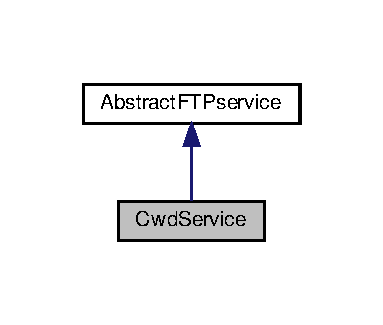
\includegraphics[width=184pt]{d1/d34/classCwdService__inherit__graph}
\end{center}
\end{figure}


Collaboration diagram for Cwd\+Service\+:\nopagebreak
\begin{figure}[H]
\begin{center}
\leavevmode
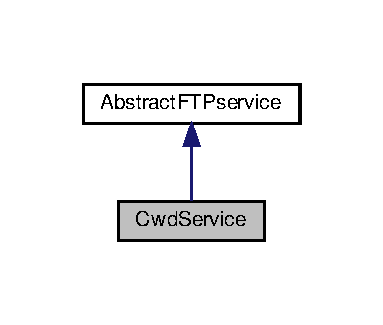
\includegraphics[width=184pt]{d5/d23/classCwdService__coll__graph}
\end{center}
\end{figure}
\subsection*{Public Member Functions}
\begin{DoxyCompactItemize}
\item 
\hyperlink{classCwdService_a88204e4221cde51198702aad17cb5b31}{Cwd\+Service} (int command\+Channel\+Socket, const Q\+String \&path)
\end{DoxyCompactItemize}
\subsection*{Additional Inherited Members}


\subsection{Detailed Description}
Service for handling C\+WD ftp command. 

\subsection{Constructor \& Destructor Documentation}
\mbox{\Hypertarget{classCwdService_a88204e4221cde51198702aad17cb5b31}\label{classCwdService_a88204e4221cde51198702aad17cb5b31}} 
\index{Cwd\+Service@{Cwd\+Service}!Cwd\+Service@{Cwd\+Service}}
\index{Cwd\+Service@{Cwd\+Service}!Cwd\+Service@{Cwd\+Service}}
\subsubsection{\texorpdfstring{Cwd\+Service()}{CwdService()}}
{\footnotesize\ttfamily Cwd\+Service\+::\+Cwd\+Service (\begin{DoxyParamCaption}\item[{int}]{command\+Channel\+Socket,  }\item[{const Q\+String \&}]{path }\end{DoxyParamCaption})}


\begin{DoxyParams}{Parameters}
{\em command\+Channel\+Socket} & Socket to communication with client on command channel \\
\hline
{\em path} & Path or name of the directory \\
\hline
\end{DoxyParams}


The documentation for this class was generated from the following files\+:\begin{DoxyCompactItemize}
\item 
src/controller/services/srv/cwdservice.\+h\item 
src/controller/services/srv/cwdservice.\+cpp\end{DoxyCompactItemize}

\hypertarget{classFileLocker}{}\section{File\+Locker Class Reference}
\label{classFileLocker}\index{File\+Locker@{File\+Locker}}


Lock files from being deleted/modified by transmission or rmdir command.  




{\ttfamily \#include $<$filelocker.\+h$>$}

\subsection*{Static Public Member Functions}
\begin{DoxyCompactItemize}
\item 
static bool \hyperlink{classFileLocker_ad8380762c767d038ec02d936bf974180}{try\+Hard\+Lock\+File} (const Q\+File\+Info \&lock\+File)
\begin{DoxyCompactList}\small\item\em Lock file from read/write/delete. \end{DoxyCompactList}\item 
static void \hyperlink{classFileLocker_a22ccc8e611b73bdfad46f410530c5ac9}{hard\+Un\+Lock\+File} (const Q\+File\+Info \&lock\+File)
\begin{DoxyCompactList}\small\item\em Unlock file for read/write/delete. \end{DoxyCompactList}\item 
static bool \hyperlink{classFileLocker_a107060898062f6990b58d0cb102551ac}{try\+Soft\+Lock\+File} (const Q\+File\+Info \&lock\+File)
\begin{DoxyCompactList}\small\item\em Lock file from write/delete. \end{DoxyCompactList}\item 
static void \hyperlink{classFileLocker_afcffcde6a3a2a410fc981c17c63fe706}{soft\+Un\+Lock\+File} (const Q\+File\+Info \&lock\+File)
\begin{DoxyCompactList}\small\item\em Unlock file for write/delete. \end{DoxyCompactList}\end{DoxyCompactItemize}


\subsection{Detailed Description}
Lock files from being deleted/modified by transmission or rmdir command. 

\subsection{Member Function Documentation}
\mbox{\Hypertarget{classFileLocker_a22ccc8e611b73bdfad46f410530c5ac9}\label{classFileLocker_a22ccc8e611b73bdfad46f410530c5ac9}} 
\index{File\+Locker@{File\+Locker}!hard\+Un\+Lock\+File@{hard\+Un\+Lock\+File}}
\index{hard\+Un\+Lock\+File@{hard\+Un\+Lock\+File}!File\+Locker@{File\+Locker}}
\subsubsection{\texorpdfstring{hard\+Un\+Lock\+File()}{hardUnLockFile()}}
{\footnotesize\ttfamily void File\+Locker\+::hard\+Un\+Lock\+File (\begin{DoxyParamCaption}\item[{const Q\+File\+Info \&}]{lock\+File }\end{DoxyParamCaption})\hspace{0.3cm}{\ttfamily [static]}}



Unlock file for read/write/delete. 


\begin{DoxyParams}{Parameters}
{\em lock\+File} & File which is locked by try\+Hard\+Lock\+File method. \\
\hline
\end{DoxyParams}
\mbox{\Hypertarget{classFileLocker_afcffcde6a3a2a410fc981c17c63fe706}\label{classFileLocker_afcffcde6a3a2a410fc981c17c63fe706}} 
\index{File\+Locker@{File\+Locker}!soft\+Un\+Lock\+File@{soft\+Un\+Lock\+File}}
\index{soft\+Un\+Lock\+File@{soft\+Un\+Lock\+File}!File\+Locker@{File\+Locker}}
\subsubsection{\texorpdfstring{soft\+Un\+Lock\+File()}{softUnLockFile()}}
{\footnotesize\ttfamily void File\+Locker\+::soft\+Un\+Lock\+File (\begin{DoxyParamCaption}\item[{const Q\+File\+Info \&}]{lock\+File }\end{DoxyParamCaption})\hspace{0.3cm}{\ttfamily [static]}}



Unlock file for write/delete. 


\begin{DoxyParams}{Parameters}
{\em lock\+File} & File which is locked by try\+Soft\+Lock\+File method. \\
\hline
\end{DoxyParams}
\mbox{\Hypertarget{classFileLocker_ad8380762c767d038ec02d936bf974180}\label{classFileLocker_ad8380762c767d038ec02d936bf974180}} 
\index{File\+Locker@{File\+Locker}!try\+Hard\+Lock\+File@{try\+Hard\+Lock\+File}}
\index{try\+Hard\+Lock\+File@{try\+Hard\+Lock\+File}!File\+Locker@{File\+Locker}}
\subsubsection{\texorpdfstring{try\+Hard\+Lock\+File()}{tryHardLockFile()}}
{\footnotesize\ttfamily bool File\+Locker\+::try\+Hard\+Lock\+File (\begin{DoxyParamCaption}\item[{const Q\+File\+Info \&}]{lock\+File }\end{DoxyParamCaption})\hspace{0.3cm}{\ttfamily [static]}}



Lock file from read/write/delete. 


\begin{DoxyParams}{Parameters}
{\em lock\+File} & File to be locked. \\
\hline
\end{DoxyParams}
\begin{DoxyReturn}{Returns}
True if file is locked. 
\end{DoxyReturn}
\mbox{\Hypertarget{classFileLocker_a107060898062f6990b58d0cb102551ac}\label{classFileLocker_a107060898062f6990b58d0cb102551ac}} 
\index{File\+Locker@{File\+Locker}!try\+Soft\+Lock\+File@{try\+Soft\+Lock\+File}}
\index{try\+Soft\+Lock\+File@{try\+Soft\+Lock\+File}!File\+Locker@{File\+Locker}}
\subsubsection{\texorpdfstring{try\+Soft\+Lock\+File()}{trySoftLockFile()}}
{\footnotesize\ttfamily bool File\+Locker\+::try\+Soft\+Lock\+File (\begin{DoxyParamCaption}\item[{const Q\+File\+Info \&}]{lock\+File }\end{DoxyParamCaption})\hspace{0.3cm}{\ttfamily [static]}}



Lock file from write/delete. 


\begin{DoxyParams}{Parameters}
{\em lock\+File} & File to be locked. \\
\hline
\end{DoxyParams}
\begin{DoxyReturn}{Returns}
True if file is locked. 
\end{DoxyReturn}


The documentation for this class was generated from the following files\+:\begin{DoxyCompactItemize}
\item 
src/ftpfilesystem/filelocker.\+h\item 
src/ftpfilesystem/filelocker.\+cpp\end{DoxyCompactItemize}

\hypertarget{structInterfaceTransmissionFileAccess_1_1FileOpeningException}{}\section{Interface\+Transmission\+File\+Access\+:\+:File\+Opening\+Exception Struct Reference}
\label{structInterfaceTransmissionFileAccess_1_1FileOpeningException}\index{Interface\+Transmission\+File\+Access\+::\+File\+Opening\+Exception@{Interface\+Transmission\+File\+Access\+::\+File\+Opening\+Exception}}


Inheritance diagram for Interface\+Transmission\+File\+Access\+:\+:File\+Opening\+Exception\+:\nopagebreak
\begin{figure}[H]
\begin{center}
\leavevmode
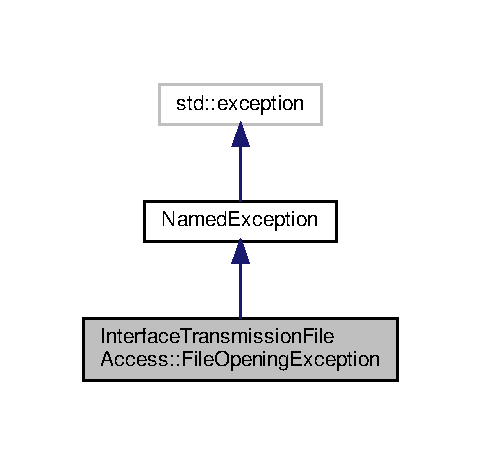
\includegraphics[width=231pt]{d5/ddb/structInterfaceTransmissionFileAccess_1_1FileOpeningException__inherit__graph}
\end{center}
\end{figure}


Collaboration diagram for Interface\+Transmission\+File\+Access\+:\+:File\+Opening\+Exception\+:\nopagebreak
\begin{figure}[H]
\begin{center}
\leavevmode
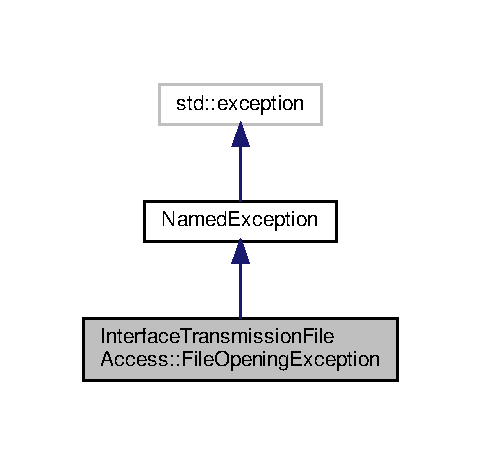
\includegraphics[width=231pt]{de/dbd/structInterfaceTransmissionFileAccess_1_1FileOpeningException__coll__graph}
\end{center}
\end{figure}
\subsection*{Public Member Functions}
\begin{DoxyCompactItemize}
\item 
\mbox{\Hypertarget{structInterfaceTransmissionFileAccess_1_1FileOpeningException_a8c847455583fb774165034c9593a55f0}\label{structInterfaceTransmissionFileAccess_1_1FileOpeningException_a8c847455583fb774165034c9593a55f0}} 
virtual const char $\ast$ {\bfseries what} () const noexcept override
\item 
\mbox{\Hypertarget{structInterfaceTransmissionFileAccess_1_1FileOpeningException_a5205856eab34cb642c85bb9130c14615}\label{structInterfaceTransmissionFileAccess_1_1FileOpeningException_a5205856eab34cb642c85bb9130c14615}} 
virtual Q\+String {\bfseries name} () override
\end{DoxyCompactItemize}


The documentation for this struct was generated from the following file\+:\begin{DoxyCompactItemize}
\item 
src/transmission/filetransmission.\+h\end{DoxyCompactItemize}

\hypertarget{structAbstractFileTransmission_1_1FileTransmissionReceiveException}{}\section{Abstract\+File\+Transmission\+:\+:File\+Transmission\+Receive\+Exception Struct Reference}
\label{structAbstractFileTransmission_1_1FileTransmissionReceiveException}\index{Abstract\+File\+Transmission\+::\+File\+Transmission\+Receive\+Exception@{Abstract\+File\+Transmission\+::\+File\+Transmission\+Receive\+Exception}}


Inheritance diagram for Abstract\+File\+Transmission\+:\+:File\+Transmission\+Receive\+Exception\+:\nopagebreak
\begin{figure}[H]
\begin{center}
\leavevmode
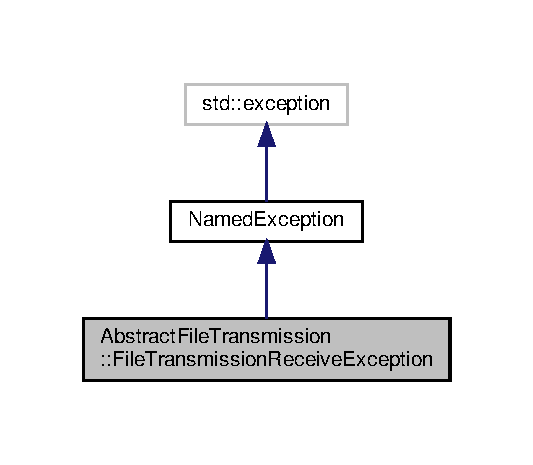
\includegraphics[width=256pt]{d6/d49/structAbstractFileTransmission_1_1FileTransmissionReceiveException__inherit__graph}
\end{center}
\end{figure}


Collaboration diagram for Abstract\+File\+Transmission\+:\+:File\+Transmission\+Receive\+Exception\+:\nopagebreak
\begin{figure}[H]
\begin{center}
\leavevmode
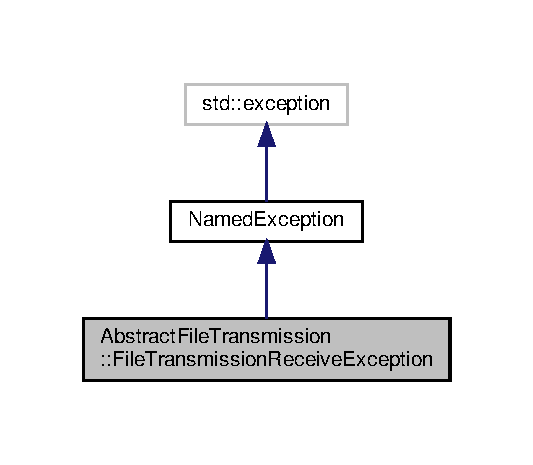
\includegraphics[width=256pt]{d6/d54/structAbstractFileTransmission_1_1FileTransmissionReceiveException__coll__graph}
\end{center}
\end{figure}
\subsection*{Public Member Functions}
\begin{DoxyCompactItemize}
\item 
\mbox{\Hypertarget{structAbstractFileTransmission_1_1FileTransmissionReceiveException_a7b941ad73573b45103edef12d9bb8aa7}\label{structAbstractFileTransmission_1_1FileTransmissionReceiveException_a7b941ad73573b45103edef12d9bb8aa7}} 
virtual const char $\ast$ {\bfseries what} () const noexcept override
\item 
\mbox{\Hypertarget{structAbstractFileTransmission_1_1FileTransmissionReceiveException_a5b32334695f716812982c4a8281071f2}\label{structAbstractFileTransmission_1_1FileTransmissionReceiveException_a5b32334695f716812982c4a8281071f2}} 
virtual Q\+String {\bfseries name} () override
\end{DoxyCompactItemize}


The documentation for this struct was generated from the following file\+:\begin{DoxyCompactItemize}
\item 
src/transmission/filetransmission.\+h\end{DoxyCompactItemize}

\hypertarget{structAbstractFileTransmission_1_1FileTransmissionSendException}{}\section{Abstract\+File\+Transmission\+:\+:File\+Transmission\+Send\+Exception Struct Reference}
\label{structAbstractFileTransmission_1_1FileTransmissionSendException}\index{Abstract\+File\+Transmission\+::\+File\+Transmission\+Send\+Exception@{Abstract\+File\+Transmission\+::\+File\+Transmission\+Send\+Exception}}


Inheritance diagram for Abstract\+File\+Transmission\+:\+:File\+Transmission\+Send\+Exception\+:\nopagebreak
\begin{figure}[H]
\begin{center}
\leavevmode
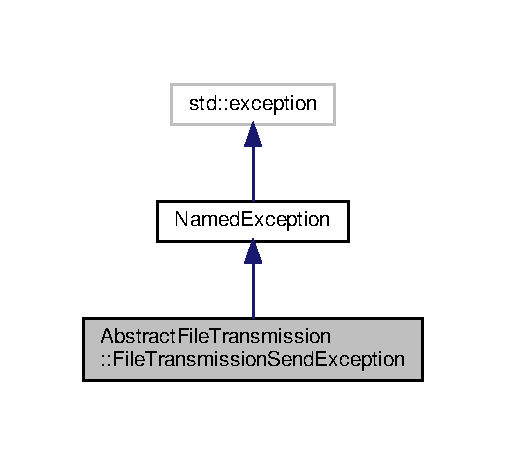
\includegraphics[width=243pt]{d6/d87/structAbstractFileTransmission_1_1FileTransmissionSendException__inherit__graph}
\end{center}
\end{figure}


Collaboration diagram for Abstract\+File\+Transmission\+:\+:File\+Transmission\+Send\+Exception\+:\nopagebreak
\begin{figure}[H]
\begin{center}
\leavevmode
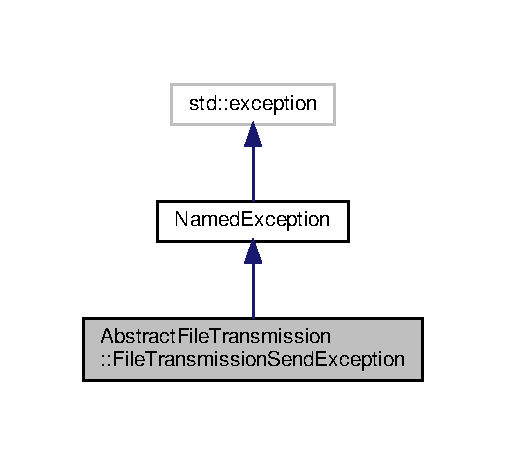
\includegraphics[width=243pt]{dd/d64/structAbstractFileTransmission_1_1FileTransmissionSendException__coll__graph}
\end{center}
\end{figure}
\subsection*{Public Member Functions}
\begin{DoxyCompactItemize}
\item 
\mbox{\Hypertarget{structAbstractFileTransmission_1_1FileTransmissionSendException_a2d795f1bc62aad88b12832ec1605bc27}\label{structAbstractFileTransmission_1_1FileTransmissionSendException_a2d795f1bc62aad88b12832ec1605bc27}} 
virtual const char $\ast$ {\bfseries what} () const noexcept override
\item 
\mbox{\Hypertarget{structAbstractFileTransmission_1_1FileTransmissionSendException_aae911a35436ec47d0ca15efb9be23149}\label{structAbstractFileTransmission_1_1FileTransmissionSendException_aae911a35436ec47d0ca15efb9be23149}} 
virtual Q\+String {\bfseries name} () override
\end{DoxyCompactItemize}


The documentation for this struct was generated from the following file\+:\begin{DoxyCompactItemize}
\item 
src/transmission/filetransmission.\+h\end{DoxyCompactItemize}

\hypertarget{classFTPconnectionWorker}{}\section{F\+T\+Pconnection\+Worker Class Reference}
\label{classFTPconnectionWorker}\index{F\+T\+Pconnection\+Worker@{F\+T\+Pconnection\+Worker}}


Manages one ftp connection.  




{\ttfamily \#include $<$ftpconnectionworker.\+h$>$}



Inheritance diagram for F\+T\+Pconnection\+Worker\+:\nopagebreak
\begin{figure}[H]
\begin{center}
\leavevmode
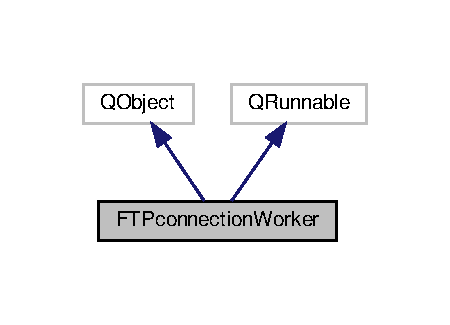
\includegraphics[width=216pt]{d2/df5/classFTPconnectionWorker__inherit__graph}
\end{center}
\end{figure}


Collaboration diagram for F\+T\+Pconnection\+Worker\+:\nopagebreak
\begin{figure}[H]
\begin{center}
\leavevmode
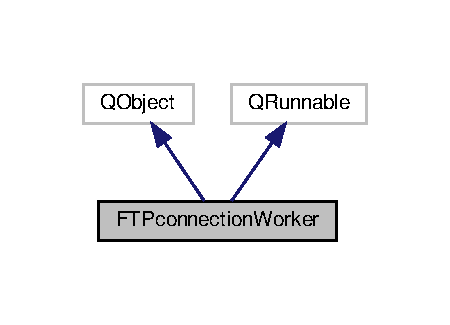
\includegraphics[width=216pt]{de/da8/classFTPconnectionWorker__coll__graph}
\end{center}
\end{figure}
\subsection*{Signals}
\begin{DoxyCompactItemize}
\item 
\mbox{\Hypertarget{classFTPconnectionWorker_a0783b9741d75098496bfd7276d37a9ea}\label{classFTPconnectionWorker_a0783b9741d75098496bfd7276d37a9ea}} 
void {\bfseries done} (int client\+Command\+Channel)
\end{DoxyCompactItemize}
\subsection*{Public Member Functions}
\begin{DoxyCompactItemize}
\item 
\hyperlink{classFTPconnectionWorker_a6763cf440da5695484f0ec06feb84b38}{F\+T\+Pconnection\+Worker} (int client\+Command\+Channel)
\item 
\mbox{\Hypertarget{classFTPconnectionWorker_a60ea10b434bcd8c7ad8e39e0f0e61ed6}\label{classFTPconnectionWorker_a60ea10b434bcd8c7ad8e39e0f0e61ed6}} 
void {\bfseries run} () override
\end{DoxyCompactItemize}
\subsection*{Static Public Member Functions}
\begin{DoxyCompactItemize}
\item 
\mbox{\Hypertarget{classFTPconnectionWorker_a3772837b65d47738e76df6078e48dab4}\label{classFTPconnectionWorker_a3772837b65d47738e76df6078e48dab4}} 
static void {\bfseries set\+Timeout\+Ms} (int value)
\item 
\mbox{\Hypertarget{classFTPconnectionWorker_a3760a2531e1fa2a5717ba4775be36dab}\label{classFTPconnectionWorker_a3760a2531e1fa2a5717ba4775be36dab}} 
static void {\bfseries set\+Bsd\+Socket\+Factory} (const \hyperlink{classInterfaceBsdSocketFactory}{Interface\+Bsd\+Socket\+Factory} \&new\+Factory)
\end{DoxyCompactItemize}


\subsection{Detailed Description}
Manages one ftp connection. 

\subsection{Constructor \& Destructor Documentation}
\mbox{\Hypertarget{classFTPconnectionWorker_a6763cf440da5695484f0ec06feb84b38}\label{classFTPconnectionWorker_a6763cf440da5695484f0ec06feb84b38}} 
\index{F\+T\+Pconnection\+Worker@{F\+T\+Pconnection\+Worker}!F\+T\+Pconnection\+Worker@{F\+T\+Pconnection\+Worker}}
\index{F\+T\+Pconnection\+Worker@{F\+T\+Pconnection\+Worker}!F\+T\+Pconnection\+Worker@{F\+T\+Pconnection\+Worker}}
\subsubsection{\texorpdfstring{F\+T\+Pconnection\+Worker()}{FTPconnectionWorker()}}
{\footnotesize\ttfamily F\+T\+Pconnection\+Worker\+::\+F\+T\+Pconnection\+Worker (\begin{DoxyParamCaption}\item[{int}]{client\+Command\+Channel }\end{DoxyParamCaption})}


\begin{DoxyParams}{Parameters}
{\em client\+Command\+Channel} & Socket to communication with client on command channel. \\
\hline
\end{DoxyParams}


The documentation for this class was generated from the following files\+:\begin{DoxyCompactItemize}
\item 
src/controller/ftpconnectionworker.\+h\item 
src/controller/ftpconnectionworker.\+cpp\end{DoxyCompactItemize}

\hypertarget{classFTPcontroller}{}\section{F\+T\+Pcontroller Class Reference}
\label{classFTPcontroller}\index{F\+T\+Pcontroller@{F\+T\+Pcontroller}}


Main F\+TP server module.  




{\ttfamily \#include $<$ftpcontroller.\+h$>$}



Inheritance diagram for F\+T\+Pcontroller\+:\nopagebreak
\begin{figure}[H]
\begin{center}
\leavevmode
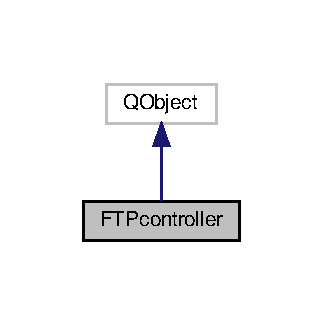
\includegraphics[width=155pt]{d8/d5c/classFTPcontroller__inherit__graph}
\end{center}
\end{figure}


Collaboration diagram for F\+T\+Pcontroller\+:\nopagebreak
\begin{figure}[H]
\begin{center}
\leavevmode
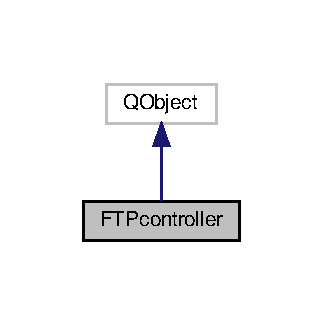
\includegraphics[width=155pt]{d9/d30/classFTPcontroller__coll__graph}
\end{center}
\end{figure}
\subsection*{Signals}
\begin{DoxyCompactItemize}
\item 
\mbox{\Hypertarget{classFTPcontroller_a83ed496fc32dff4f3257098b0589dd85}\label{classFTPcontroller_a83ed496fc32dff4f3257098b0589dd85}} 
void {\bfseries new\+Connection} (int client\+Socket)
\end{DoxyCompactItemize}
\subsection*{Public Member Functions}
\begin{DoxyCompactItemize}
\item 
\mbox{\Hypertarget{classFTPcontroller_aee9902900896bb6d19819cf33835e938}\label{classFTPcontroller_aee9902900896bb6d19819cf33835e938}} 
{\bfseries F\+T\+Pcontroller} (const Q\+String \&address, int port)
\item 
\mbox{\Hypertarget{classFTPcontroller_aa828486ab01a8f6bacc7c99585294a50}\label{classFTPcontroller_aa828486ab01a8f6bacc7c99585294a50}} 
void {\bfseries start} ()
\end{DoxyCompactItemize}
\subsection*{Static Public Member Functions}
\begin{DoxyCompactItemize}
\item 
\mbox{\Hypertarget{classFTPcontroller_acea265b87e5d776e4943e71888411271}\label{classFTPcontroller_acea265b87e5d776e4943e71888411271}} 
static void {\bfseries set\+Bsd\+Socket\+Factory} (const \hyperlink{classInterfaceBsdSocketFactory}{Interface\+Bsd\+Socket\+Factory} \&new\+Factory)
\end{DoxyCompactItemize}


\subsection{Detailed Description}
Main F\+TP server module. 

The documentation for this class was generated from the following files\+:\begin{DoxyCompactItemize}
\item 
src/controller/ftpcontroller.\+h\item 
src/controller/ftpcontroller.\+cpp\end{DoxyCompactItemize}

\hypertarget{classFTPfileSystemDefault}{}\section{F\+T\+Pfile\+System\+Default Class Reference}
\label{classFTPfileSystemDefault}\index{F\+T\+Pfile\+System\+Default@{F\+T\+Pfile\+System\+Default}}


Default implementation of ftp filesystem interface, provide private user file space.  




{\ttfamily \#include $<$ftpfilesystem.\+h$>$}



Inheritance diagram for F\+T\+Pfile\+System\+Default\+:\nopagebreak
\begin{figure}[H]
\begin{center}
\leavevmode
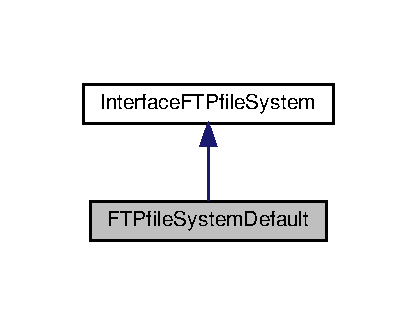
\includegraphics[width=200pt]{d9/d6b/classFTPfileSystemDefault__inherit__graph}
\end{center}
\end{figure}


Collaboration diagram for F\+T\+Pfile\+System\+Default\+:\nopagebreak
\begin{figure}[H]
\begin{center}
\leavevmode
\includegraphics[width=200pt]{da/d1c/classFTPfileSystemDefault__coll__graph}
\end{center}
\end{figure}
\subsection*{Public Member Functions}
\begin{DoxyCompactItemize}
\item 
\mbox{\Hypertarget{classFTPfileSystemDefault_ac815690308b16bad4ed9754ac462ff29}\label{classFTPfileSystemDefault_ac815690308b16bad4ed9754ac462ff29}} 
{\bfseries F\+T\+Pfile\+System\+Default} (const Q\+File\+Info \&begin\+User\+File\+Space)
\item 
\mbox{\Hypertarget{classFTPfileSystemDefault_a8133a418858f97b9fb5a60efdc47d5c1}\label{classFTPfileSystemDefault_a8133a418858f97b9fb5a60efdc47d5c1}} 
virtual Q\+String {\bfseries print\+Working\+Directory} (bool relative\+Path) const override
\item 
\mbox{\Hypertarget{classFTPfileSystemDefault_a8a217c19ac3a375033790b50f4ea5007}\label{classFTPfileSystemDefault_a8a217c19ac3a375033790b50f4ea5007}} 
virtual bool {\bfseries change\+Absolute\+Working\+Directory} (const Q\+String \&path) override
\item 
\mbox{\Hypertarget{classFTPfileSystemDefault_aedfd0d666deeb47c00204c72fd758450}\label{classFTPfileSystemDefault_aedfd0d666deeb47c00204c72fd758450}} 
virtual bool {\bfseries change\+Relative\+Root\+Working\+Directory} (const Q\+String \&path) override
\item 
\mbox{\Hypertarget{classFTPfileSystemDefault_a5760b8bee8657ea1be5b789a695b22c1}\label{classFTPfileSystemDefault_a5760b8bee8657ea1be5b789a695b22c1}} 
virtual bool {\bfseries change\+Relative\+Current\+Working\+Directory} (const Q\+String \&path) override
\item 
\mbox{\Hypertarget{classFTPfileSystemDefault_a93e87fb1c7cf499e9558b611ee514259}\label{classFTPfileSystemDefault_a93e87fb1c7cf499e9558b611ee514259}} 
virtual bool {\bfseries change\+Working\+Directory\+To\+Parent} () override
\item 
\mbox{\Hypertarget{classFTPfileSystemDefault_a7834af9643939e5a586a28eb23198abe}\label{classFTPfileSystemDefault_a7834af9643939e5a586a28eb23198abe}} 
virtual bool {\bfseries mkdir\+WD} (const Q\+String \&name) override
\item 
\mbox{\Hypertarget{classFTPfileSystemDefault_a8b9682168e31ded3c24088dca5cf9c57}\label{classFTPfileSystemDefault_a8b9682168e31ded3c24088dca5cf9c57}} 
virtual bool {\bfseries mkdir\+Relative\+Root\+Path} (const Q\+String \&path) override
\item 
\mbox{\Hypertarget{classFTPfileSystemDefault_a9e2b21a3d300413370aa81b00c7360d9}\label{classFTPfileSystemDefault_a9e2b21a3d300413370aa81b00c7360d9}} 
virtual bool {\bfseries rmdir\+WD} (const Q\+String \&name) override
\item 
\mbox{\Hypertarget{classFTPfileSystemDefault_aae68afe3a1fc386c36bca2e4954bc0e3}\label{classFTPfileSystemDefault_aae68afe3a1fc386c36bca2e4954bc0e3}} 
virtual bool {\bfseries rmdir\+Relative\+Root\+Path} (const Q\+String \&path) override
\item 
\mbox{\Hypertarget{classFTPfileSystemDefault_a6168101554693a5f21a4d85958ec11a4}\label{classFTPfileSystemDefault_a6168101554693a5f21a4d85958ec11a4}} 
virtual Q\+String\+List {\bfseries get\+Linux\+Files\+Info\+List\+In\+Working\+Directory} () override
\item 
\mbox{\Hypertarget{classFTPfileSystemDefault_ae0fbf7bf88b89f3df913c1ce7405f8a1}\label{classFTPfileSystemDefault_ae0fbf7bf88b89f3df913c1ce7405f8a1}} 
virtual Q\+String\+List {\bfseries get\+Linux\+Files\+Info\+List\+In\+Relative\+Path} (const Q\+String \&path) override
\item 
\mbox{\Hypertarget{classFTPfileSystemDefault_a9a85a8297bb3fd9141807a0cef70ab84}\label{classFTPfileSystemDefault_a9a85a8297bb3fd9141807a0cef70ab84}} 
virtual Q\+Dir {\bfseries get\+Root\+Dir} () const override
\item 
\mbox{\Hypertarget{classFTPfileSystemDefault_aafa723712bbbed51e29658fa36c0f9ad}\label{classFTPfileSystemDefault_aafa723712bbbed51e29658fa36c0f9ad}} 
virtual Q\+Dir {\bfseries get\+Actual\+Dir} () const override
\end{DoxyCompactItemize}


\subsection{Detailed Description}
Default implementation of ftp filesystem interface, provide private user file space. 

The documentation for this class was generated from the following files\+:\begin{DoxyCompactItemize}
\item 
src/ftpfilesystem/ftpfilesystem.\+h\item 
src/ftpfilesystem/ftpfilesystem.\+cpp\end{DoxyCompactItemize}

\hypertarget{classInterfaceAccountDatabase}{}\section{Interface\+Account\+Database Class Reference}
\label{classInterfaceAccountDatabase}\index{Interface\+Account\+Database@{Interface\+Account\+Database}}


Inheritance diagram for Interface\+Account\+Database\+:\nopagebreak
\begin{figure}[H]
\begin{center}
\leavevmode
\includegraphics[width=213pt]{d0/dcd/classInterfaceAccountDatabase__inherit__graph}
\end{center}
\end{figure}
\subsection*{Data Structures}
\begin{DoxyCompactItemize}
\item 
struct \hyperlink{structInterfaceAccountDatabase_1_1AccountExistsException}{Account\+Exists\+Exception}
\item 
struct \hyperlink{structInterfaceAccountDatabase_1_1AccountNotFoundException}{Account\+Not\+Found\+Exception}
\end{DoxyCompactItemize}
\subsection*{Public Member Functions}
\begin{DoxyCompactItemize}
\item 
\mbox{\Hypertarget{classInterfaceAccountDatabase_a54f1a9870a88598e8953759541a0b5cc}\label{classInterfaceAccountDatabase_a54f1a9870a88598e8953759541a0b5cc}} 
virtual void {\bfseries add\+Account\+Info} (const \hyperlink{classAccountInfo}{Account\+Info} \&account\+Info)=0
\item 
\mbox{\Hypertarget{classInterfaceAccountDatabase_a198df5c7964870e0feee9cf26a7dca7a}\label{classInterfaceAccountDatabase_a198df5c7964870e0feee9cf26a7dca7a}} 
virtual \hyperlink{classAccountInfo}{Account\+Info} {\bfseries get\+Account\+Info} (int command\+Channel\+Socket)=0
\item 
\mbox{\Hypertarget{classInterfaceAccountDatabase_a6984fa5e427b80b6710b0cf122e52579}\label{classInterfaceAccountDatabase_a6984fa5e427b80b6710b0cf122e52579}} 
virtual void {\bfseries set\+Account\+Info} (const \hyperlink{classAccountInfo}{Account\+Info} \&account\+Info)=0
\item 
\mbox{\Hypertarget{classInterfaceAccountDatabase_a182c1d1ca50325dc73a5e00cafe4d0f2}\label{classInterfaceAccountDatabase_a182c1d1ca50325dc73a5e00cafe4d0f2}} 
virtual void {\bfseries del\+Account\+Info} (int command\+Channel\+Socket)=0
\item 
\mbox{\Hypertarget{classInterfaceAccountDatabase_af1489731737b67931d0601c964fa5883}\label{classInterfaceAccountDatabase_af1489731737b67931d0601c964fa5883}} 
virtual void {\bfseries reset\+Database} ()=0
\end{DoxyCompactItemize}


The documentation for this class was generated from the following files\+:\begin{DoxyCompactItemize}
\item 
src/account/accountdatabase.\+h\item 
src/account/accountdatabase.\+cpp\end{DoxyCompactItemize}

\hypertarget{classInterfaceBsdSocketFactory}{}\section{Interface\+Bsd\+Socket\+Factory Class Reference}
\label{classInterfaceBsdSocketFactory}\index{Interface\+Bsd\+Socket\+Factory@{Interface\+Bsd\+Socket\+Factory}}


Inheritance diagram for Interface\+Bsd\+Socket\+Factory\+:\nopagebreak
\begin{figure}[H]
\begin{center}
\leavevmode
\includegraphics[width=216pt]{dc/dfa/classInterfaceBsdSocketFactory__inherit__graph}
\end{center}
\end{figure}
\subsection*{Public Member Functions}
\begin{DoxyCompactItemize}
\item 
\mbox{\Hypertarget{classInterfaceBsdSocketFactory_aa259ed6a1bd32e3bf77e97fc150cd54a}\label{classInterfaceBsdSocketFactory_aa259ed6a1bd32e3bf77e97fc150cd54a}} 
virtual int {\bfseries socket} (int \+\_\+\+\_\+domain, int \+\_\+\+\_\+type, int \+\_\+\+\_\+protocol)=0
\item 
\mbox{\Hypertarget{classInterfaceBsdSocketFactory_a389576ba0564ce79ce650f300921b533}\label{classInterfaceBsdSocketFactory_a389576ba0564ce79ce650f300921b533}} 
virtual int {\bfseries connect} (int \+\_\+\+\_\+fd, \+\_\+\+\_\+\+C\+O\+N\+S\+T\+\_\+\+S\+O\+C\+K\+A\+D\+D\+R\+\_\+\+A\+RG \+\_\+\+\_\+addr, socklen\+\_\+t \+\_\+\+\_\+len)=0
\item 
\mbox{\Hypertarget{classInterfaceBsdSocketFactory_a762639f3055ce6e4b21a092f96d6e515}\label{classInterfaceBsdSocketFactory_a762639f3055ce6e4b21a092f96d6e515}} 
virtual ssize\+\_\+t {\bfseries write} (int \+\_\+\+\_\+fd, const void $\ast$\+\_\+\+\_\+buf, size\+\_\+t \+\_\+\+\_\+n)=0
\item 
\mbox{\Hypertarget{classInterfaceBsdSocketFactory_a8b2965f642070600bed86e4664beec8b}\label{classInterfaceBsdSocketFactory_a8b2965f642070600bed86e4664beec8b}} 
virtual ssize\+\_\+t {\bfseries read} (int \+\_\+\+\_\+fd, void $\ast$\+\_\+\+\_\+buf, size\+\_\+t \+\_\+\+\_\+nbytes)=0
\item 
\mbox{\Hypertarget{classInterfaceBsdSocketFactory_a6e38160aac35e1f64b35c205de2f9452}\label{classInterfaceBsdSocketFactory_a6e38160aac35e1f64b35c205de2f9452}} 
virtual int {\bfseries bind} (int \+\_\+\+\_\+fd, \+\_\+\+\_\+\+C\+O\+N\+S\+T\+\_\+\+S\+O\+C\+K\+A\+D\+D\+R\+\_\+\+A\+RG \+\_\+\+\_\+addr, socklen\+\_\+t \+\_\+\+\_\+len)=0
\item 
\mbox{\Hypertarget{classInterfaceBsdSocketFactory_a2f2c6dbbb9d1f7fa0a42f0039178836c}\label{classInterfaceBsdSocketFactory_a2f2c6dbbb9d1f7fa0a42f0039178836c}} 
virtual int {\bfseries listen} (int \+\_\+\+\_\+fd, int \+\_\+\+\_\+n)=0
\item 
\mbox{\Hypertarget{classInterfaceBsdSocketFactory_a3be681ec6b076c808a8563daf481c118}\label{classInterfaceBsdSocketFactory_a3be681ec6b076c808a8563daf481c118}} 
virtual int {\bfseries accept} (int \+\_\+\+\_\+fd, \+\_\+\+\_\+\+S\+O\+C\+K\+A\+D\+D\+R\+\_\+\+A\+RG \+\_\+\+\_\+addr, socklen\+\_\+t $\ast$\+\_\+\+\_\+restrict \+\_\+\+\_\+addr\+\_\+len)=0
\item 
\mbox{\Hypertarget{classInterfaceBsdSocketFactory_a2cb114ed8514fdb9a5a231a14e36ef5a}\label{classInterfaceBsdSocketFactory_a2cb114ed8514fdb9a5a231a14e36ef5a}} 
virtual int {\bfseries close} (int \+\_\+\+\_\+fd)=0
\item 
\mbox{\Hypertarget{classInterfaceBsdSocketFactory_a6081647e7bcffdb4af53cc71ff42f792}\label{classInterfaceBsdSocketFactory_a6081647e7bcffdb4af53cc71ff42f792}} 
virtual int {\bfseries getsockopt} (int \+\_\+\+\_\+fd, int \+\_\+\+\_\+level, int \+\_\+\+\_\+optname, void $\ast$\+\_\+\+\_\+restrict \+\_\+\+\_\+optval, socklen\+\_\+t $\ast$\+\_\+\+\_\+restrict \+\_\+\+\_\+optlen)=0
\item 
\mbox{\Hypertarget{classInterfaceBsdSocketFactory_aa58c4e561966713dc3b64c31a7d65adb}\label{classInterfaceBsdSocketFactory_aa58c4e561966713dc3b64c31a7d65adb}} 
virtual \hyperlink{classInterfaceBsdSocketFactory}{Interface\+Bsd\+Socket\+Factory} $\ast$ {\bfseries clone} () const
\end{DoxyCompactItemize}
\subsection*{Protected Member Functions}
\begin{DoxyCompactItemize}
\item 
\mbox{\Hypertarget{classInterfaceBsdSocketFactory_aa6918ad69cb7f660a8e79643f2ebe8ef}\label{classInterfaceBsdSocketFactory_aa6918ad69cb7f660a8e79643f2ebe8ef}} 
virtual \hyperlink{classInterfaceBsdSocketFactory}{Interface\+Bsd\+Socket\+Factory} $\ast$ {\bfseries do\+Clone} () const =0
\end{DoxyCompactItemize}


The documentation for this class was generated from the following file\+:\begin{DoxyCompactItemize}
\item 
src/bsdsocket/bsdsocketfactory.\+h\end{DoxyCompactItemize}

\hypertarget{classInterfaceFTPfileSystem}{}\section{Interface\+F\+T\+Pfile\+System Class Reference}
\label{classInterfaceFTPfileSystem}\index{Interface\+F\+T\+Pfile\+System@{Interface\+F\+T\+Pfile\+System}}


Inheritance diagram for Interface\+F\+T\+Pfile\+System\+:\nopagebreak
\begin{figure}[H]
\begin{center}
\leavevmode
\includegraphics[width=200pt]{d1/d0b/classInterfaceFTPfileSystem__inherit__graph}
\end{center}
\end{figure}
\subsection*{Data Structures}
\begin{DoxyCompactItemize}
\item 
struct \hyperlink{structInterfaceFTPfileSystem_1_1WrongRootDirPathException}{Wrong\+Root\+Dir\+Path\+Exception}
\end{DoxyCompactItemize}
\subsection*{Public Member Functions}
\begin{DoxyCompactItemize}
\item 
\mbox{\Hypertarget{classInterfaceFTPfileSystem_a99df9cb164e909a24b6c9ec353b220ea}\label{classInterfaceFTPfileSystem_a99df9cb164e909a24b6c9ec353b220ea}} 
virtual Q\+String {\bfseries print\+Working\+Directory} (bool relative\+Path) const =0
\item 
\mbox{\Hypertarget{classInterfaceFTPfileSystem_a8b51dbfdb53344cd868547fff3d8f066}\label{classInterfaceFTPfileSystem_a8b51dbfdb53344cd868547fff3d8f066}} 
virtual bool {\bfseries change\+Absolute\+Working\+Directory} (const Q\+String \&path)=0
\item 
\mbox{\Hypertarget{classInterfaceFTPfileSystem_a385969b025d97d5bbc2c9d620ea41c11}\label{classInterfaceFTPfileSystem_a385969b025d97d5bbc2c9d620ea41c11}} 
virtual bool {\bfseries change\+Relative\+Root\+Working\+Directory} (const Q\+String \&path)=0
\item 
\mbox{\Hypertarget{classInterfaceFTPfileSystem_a0db5681012b9b09873043a2f84de180c}\label{classInterfaceFTPfileSystem_a0db5681012b9b09873043a2f84de180c}} 
virtual bool {\bfseries change\+Relative\+Current\+Working\+Directory} (const Q\+String \&path)=0
\item 
\mbox{\Hypertarget{classInterfaceFTPfileSystem_a3a5704f8e6c964923426047bdef1cb33}\label{classInterfaceFTPfileSystem_a3a5704f8e6c964923426047bdef1cb33}} 
virtual bool {\bfseries change\+Working\+Directory\+To\+Parent} ()=0
\item 
\mbox{\Hypertarget{classInterfaceFTPfileSystem_a1b4df812b4251df5d0928c11576d6132}\label{classInterfaceFTPfileSystem_a1b4df812b4251df5d0928c11576d6132}} 
virtual bool {\bfseries mkdir\+WD} (const Q\+String \&name)=0
\item 
\mbox{\Hypertarget{classInterfaceFTPfileSystem_ab6758fa3bfaa9d47b9d20cec84b8e141}\label{classInterfaceFTPfileSystem_ab6758fa3bfaa9d47b9d20cec84b8e141}} 
virtual bool {\bfseries mkdir\+Relative\+Root\+Path} (const Q\+String \&path)=0
\item 
\mbox{\Hypertarget{classInterfaceFTPfileSystem_a15f1107934dfa3ebdee659bb350495d8}\label{classInterfaceFTPfileSystem_a15f1107934dfa3ebdee659bb350495d8}} 
virtual bool {\bfseries rmdir\+WD} (const Q\+String \&name)=0
\item 
\mbox{\Hypertarget{classInterfaceFTPfileSystem_a275dd61645adb1912af078f27e4ff167}\label{classInterfaceFTPfileSystem_a275dd61645adb1912af078f27e4ff167}} 
virtual bool {\bfseries rmdir\+Relative\+Root\+Path} (const Q\+String \&path)=0
\item 
\mbox{\Hypertarget{classInterfaceFTPfileSystem_a41b8ae07679067b4271d5435a8416ebf}\label{classInterfaceFTPfileSystem_a41b8ae07679067b4271d5435a8416ebf}} 
virtual Q\+String\+List {\bfseries get\+Linux\+Files\+Info\+List\+In\+Working\+Directory} ()=0
\item 
\mbox{\Hypertarget{classInterfaceFTPfileSystem_a01b1cd4f92a23fe9659102b82d11135c}\label{classInterfaceFTPfileSystem_a01b1cd4f92a23fe9659102b82d11135c}} 
virtual Q\+String\+List {\bfseries get\+Linux\+Files\+Info\+List\+In\+Relative\+Path} (const Q\+String \&path)=0
\item 
\mbox{\Hypertarget{classInterfaceFTPfileSystem_a798f5c44f6b41df61da64f24824edf36}\label{classInterfaceFTPfileSystem_a798f5c44f6b41df61da64f24824edf36}} 
virtual Q\+Dir {\bfseries get\+Root\+Dir} () const =0
\item 
\mbox{\Hypertarget{classInterfaceFTPfileSystem_a660fbd9b5c7eb9b71a490aaa314ab1ac}\label{classInterfaceFTPfileSystem_a660fbd9b5c7eb9b71a490aaa314ab1ac}} 
virtual Q\+Dir {\bfseries get\+Actual\+Dir} () const =0
\end{DoxyCompactItemize}


The documentation for this class was generated from the following file\+:\begin{DoxyCompactItemize}
\item 
src/ftpfilesystem/ftpfilesystem.\+h\end{DoxyCompactItemize}

\hypertarget{classInterfaceTransmissionFileAccess}{}\section{Interface\+Transmission\+File\+Access Class Reference}
\label{classInterfaceTransmissionFileAccess}\index{Interface\+Transmission\+File\+Access@{Interface\+Transmission\+File\+Access}}


Inheritance diagram for Interface\+Transmission\+File\+Access\+:\nopagebreak
\begin{figure}[H]
\begin{center}
\leavevmode
\includegraphics[width=350pt]{d1/dd6/classInterfaceTransmissionFileAccess__inherit__graph}
\end{center}
\end{figure}
\subsection*{Data Structures}
\begin{DoxyCompactItemize}
\item 
struct \hyperlink{structInterfaceTransmissionFileAccess_1_1FileOpeningException}{File\+Opening\+Exception}
\end{DoxyCompactItemize}
\subsection*{Public Types}
\begin{DoxyCompactItemize}
\item 
\mbox{\Hypertarget{classInterfaceTransmissionFileAccess_ad55c52a834e6c0832685a5a351ee705d}\label{classInterfaceTransmissionFileAccess_ad55c52a834e6c0832685a5a351ee705d}} 
using {\bfseries data\+\_\+size} = size\+\_\+t
\item 
\mbox{\Hypertarget{classInterfaceTransmissionFileAccess_ad01badb0873f5db255889ad20115f5c3}\label{classInterfaceTransmissionFileAccess_ad01badb0873f5db255889ad20115f5c3}} 
using {\bfseries Buffer\+Info} = Q\+Pair$<$ Abstract\+File\+Transmission\+::\+External\+Buffer, data\+\_\+size $>$
\end{DoxyCompactItemize}
\subsection*{Public Member Functions}
\begin{DoxyCompactItemize}
\item 
virtual void \hyperlink{classInterfaceTransmissionFileAccess_a8c423ccb527b1dda62c798a75b6eb690}{init} (const Q\+File \&file)=0
\begin{DoxyCompactList}\small\item\em Open file. \end{DoxyCompactList}\item 
\mbox{\Hypertarget{classInterfaceTransmissionFileAccess_ab23bc8abfef07a7f30f05e87b25bbcfd}\label{classInterfaceTransmissionFileAccess_ab23bc8abfef07a7f30f05e87b25bbcfd}} 
virtual void \hyperlink{classInterfaceTransmissionFileAccess_ab23bc8abfef07a7f30f05e87b25bbcfd}{clean\+Up} ()=0
\begin{DoxyCompactList}\small\item\em Close file. \end{DoxyCompactList}\end{DoxyCompactItemize}


\subsection{Member Function Documentation}
\mbox{\Hypertarget{classInterfaceTransmissionFileAccess_a8c423ccb527b1dda62c798a75b6eb690}\label{classInterfaceTransmissionFileAccess_a8c423ccb527b1dda62c798a75b6eb690}} 
\index{Interface\+Transmission\+File\+Access@{Interface\+Transmission\+File\+Access}!init@{init}}
\index{init@{init}!Interface\+Transmission\+File\+Access@{Interface\+Transmission\+File\+Access}}
\subsubsection{\texorpdfstring{init()}{init()}}
{\footnotesize\ttfamily virtual void Interface\+Transmission\+File\+Access\+::init (\begin{DoxyParamCaption}\item[{const Q\+File \&}]{file }\end{DoxyParamCaption})\hspace{0.3cm}{\ttfamily [pure virtual]}}



Open file. 


\begin{DoxyParams}{Parameters}
{\em file} & File to be read/write \\
\hline
\end{DoxyParams}


Implemented in \hyperlink{classBinaryTransmissionWriter_a40cc3d88d6501af5db2ed2acd05caacc}{Binary\+Transmission\+Writer}, \hyperlink{classAsciiTransmissionWriter_af9a2b271e8e051b7dbd266ba8207b4e7}{Ascii\+Transmission\+Writer}, \hyperlink{classBinaryTransmissionReader_a28c85fe81913ccb4ba6aee44d84dbf7d}{Binary\+Transmission\+Reader}, and \hyperlink{classAsciiTransmissionReader_ab0c198c17eded2a978d974c01aebae37}{Ascii\+Transmission\+Reader}.



The documentation for this class was generated from the following file\+:\begin{DoxyCompactItemize}
\item 
src/transmission/filetransmission.\+h\end{DoxyCompactItemize}

\hypertarget{classInterfaceTransmissionReader}{}\section{Interface\+Transmission\+Reader Class Reference}
\label{classInterfaceTransmissionReader}\index{Interface\+Transmission\+Reader@{Interface\+Transmission\+Reader}}


Inheritance diagram for Interface\+Transmission\+Reader\+:\nopagebreak
\begin{figure}[H]
\begin{center}
\leavevmode
\includegraphics[width=350pt]{d1/dce/classInterfaceTransmissionReader__inherit__graph}
\end{center}
\end{figure}


Collaboration diagram for Interface\+Transmission\+Reader\+:\nopagebreak
\begin{figure}[H]
\begin{center}
\leavevmode
\includegraphics[width=225pt]{db/d1d/classInterfaceTransmissionReader__coll__graph}
\end{center}
\end{figure}
\subsection*{Public Member Functions}
\begin{DoxyCompactItemize}
\item 
virtual Buffer\+Info \hyperlink{classInterfaceTransmissionReader_ab8733fbc3a4f6dc8279c363212fd3f51}{read\+Data\+Portion} ()=0
\begin{DoxyCompactList}\small\item\em Read data from the file and write them to the buffer. \end{DoxyCompactList}\item 
\mbox{\Hypertarget{classInterfaceTransmissionReader_ad14bc1782e5d39da2f982e726cb4f51c}\label{classInterfaceTransmissionReader_ad14bc1782e5d39da2f982e726cb4f51c}} 
virtual bool {\bfseries is\+End\+Of\+File} ()=0
\end{DoxyCompactItemize}
\subsection*{Additional Inherited Members}


\subsection{Member Function Documentation}
\mbox{\Hypertarget{classInterfaceTransmissionReader_ab8733fbc3a4f6dc8279c363212fd3f51}\label{classInterfaceTransmissionReader_ab8733fbc3a4f6dc8279c363212fd3f51}} 
\index{Interface\+Transmission\+Reader@{Interface\+Transmission\+Reader}!read\+Data\+Portion@{read\+Data\+Portion}}
\index{read\+Data\+Portion@{read\+Data\+Portion}!Interface\+Transmission\+Reader@{Interface\+Transmission\+Reader}}
\subsubsection{\texorpdfstring{read\+Data\+Portion()}{readDataPortion()}}
{\footnotesize\ttfamily virtual Buffer\+Info Interface\+Transmission\+Reader\+::read\+Data\+Portion (\begin{DoxyParamCaption}{ }\end{DoxyParamCaption})\hspace{0.3cm}{\ttfamily [pure virtual]}}



Read data from the file and write them to the buffer. 

\begin{DoxyReturn}{Returns}
Buffer with data size. 
\end{DoxyReturn}


Implemented in \hyperlink{classBinaryTransmissionReader_a003a0b7a500a15ddfc573e6f54006b0c}{Binary\+Transmission\+Reader}, and \hyperlink{classAsciiTransmissionReader_a5fd477415e273e4943caac08e8b0a7e5}{Ascii\+Transmission\+Reader}.



The documentation for this class was generated from the following file\+:\begin{DoxyCompactItemize}
\item 
src/transmission/filetransmission.\+h\end{DoxyCompactItemize}

\hypertarget{classInterfaceTransmissionWriter}{}\section{Interface\+Transmission\+Writer Class Reference}
\label{classInterfaceTransmissionWriter}\index{Interface\+Transmission\+Writer@{Interface\+Transmission\+Writer}}


Inheritance diagram for Interface\+Transmission\+Writer\+:\nopagebreak
\begin{figure}[H]
\begin{center}
\leavevmode
\includegraphics[width=350pt]{de/d9f/classInterfaceTransmissionWriter__inherit__graph}
\end{center}
\end{figure}


Collaboration diagram for Interface\+Transmission\+Writer\+:\nopagebreak
\begin{figure}[H]
\begin{center}
\leavevmode
\includegraphics[width=220pt]{da/d88/classInterfaceTransmissionWriter__coll__graph}
\end{center}
\end{figure}
\subsection*{Public Member Functions}
\begin{DoxyCompactItemize}
\item 
virtual void \hyperlink{classInterfaceTransmissionWriter_a024c3a22d937e659259f2eb242b3ea97}{write\+Data\+Portion} (Buffer\+Info info)=0
\begin{DoxyCompactList}\small\item\em Read data from the buffer and write them to the file. \end{DoxyCompactList}\end{DoxyCompactItemize}
\subsection*{Additional Inherited Members}


\subsection{Member Function Documentation}
\mbox{\Hypertarget{classInterfaceTransmissionWriter_a024c3a22d937e659259f2eb242b3ea97}\label{classInterfaceTransmissionWriter_a024c3a22d937e659259f2eb242b3ea97}} 
\index{Interface\+Transmission\+Writer@{Interface\+Transmission\+Writer}!write\+Data\+Portion@{write\+Data\+Portion}}
\index{write\+Data\+Portion@{write\+Data\+Portion}!Interface\+Transmission\+Writer@{Interface\+Transmission\+Writer}}
\subsubsection{\texorpdfstring{write\+Data\+Portion()}{writeDataPortion()}}
{\footnotesize\ttfamily virtual void Interface\+Transmission\+Writer\+::write\+Data\+Portion (\begin{DoxyParamCaption}\item[{Buffer\+Info}]{info }\end{DoxyParamCaption})\hspace{0.3cm}{\ttfamily [pure virtual]}}



Read data from the buffer and write them to the file. 


\begin{DoxyParams}{Parameters}
{\em info} & Buffer with data size. \\
\hline
\end{DoxyParams}


Implemented in \hyperlink{classBinaryTransmissionWriter_aaeee88a165c1a53ef89849c08df6a5e1}{Binary\+Transmission\+Writer}, and \hyperlink{classAsciiTransmissionWriter_a49127d2b72eceeb35211d91601434a27}{Ascii\+Transmission\+Writer}.



The documentation for this class was generated from the following file\+:\begin{DoxyCompactItemize}
\item 
src/transmission/filetransmission.\+h\end{DoxyCompactItemize}

\hypertarget{classListCmd}{}\section{List\+Cmd Class Reference}
\label{classListCmd}\index{List\+Cmd@{List\+Cmd}}


Send information to the data communication channel about files in directory, or specified file. Directory can be specified or not -\/ then it implies the user\textquotesingle{}s current working directory.  




{\ttfamily \#include $<$listcmd.\+h$>$}



Inheritance diagram for List\+Cmd\+:\nopagebreak
\begin{figure}[H]
\begin{center}
\leavevmode
\includegraphics[width=195pt]{d9/d6f/classListCmd__inherit__graph}
\end{center}
\end{figure}


Collaboration diagram for List\+Cmd\+:\nopagebreak
\begin{figure}[H]
\begin{center}
\leavevmode
\includegraphics[width=195pt]{df/d4b/classListCmd__coll__graph}
\end{center}
\end{figure}
\subsection*{Public Member Functions}
\begin{DoxyCompactItemize}
\item 
\hyperlink{classListCmd_a55f022f10e1c67886dcb1f388e792ccd}{List\+Cmd} (int command\+Communication\+Socket, const Q\+String \&path)
\item 
\mbox{\Hypertarget{classListCmd_a70c2a805bc55b38b325d7866fc749771}\label{classListCmd_a70c2a805bc55b38b325d7866fc749771}} 
virtual void {\bfseries execute} () override
\item 
\mbox{\Hypertarget{classListCmd_aaf08f313961ba78c646ede0d1acdeb86}\label{classListCmd_aaf08f313961ba78c646ede0d1acdeb86}} 
void {\bfseries set\+Bsd\+Socket\+Factory} (const \hyperlink{classInterfaceBsdSocketFactory}{Interface\+Bsd\+Socket\+Factory} \&new\+Bsd\+Socket\+Factory)
\end{DoxyCompactItemize}
\subsection*{Additional Inherited Members}


\subsection{Detailed Description}
Send information to the data communication channel about files in directory, or specified file. Directory can be specified or not -\/ then it implies the user\textquotesingle{}s current working directory. 

\subsection{Constructor \& Destructor Documentation}
\mbox{\Hypertarget{classListCmd_a55f022f10e1c67886dcb1f388e792ccd}\label{classListCmd_a55f022f10e1c67886dcb1f388e792ccd}} 
\index{List\+Cmd@{List\+Cmd}!List\+Cmd@{List\+Cmd}}
\index{List\+Cmd@{List\+Cmd}!List\+Cmd@{List\+Cmd}}
\subsubsection{\texorpdfstring{List\+Cmd()}{ListCmd()}}
{\footnotesize\ttfamily List\+Cmd\+::\+List\+Cmd (\begin{DoxyParamCaption}\item[{int}]{command\+Communication\+Socket,  }\item[{const Q\+String \&}]{path }\end{DoxyParamCaption})}


\begin{DoxyParams}{Parameters}
{\em command\+Communication\+Socket} & Socket to communication with client on command channel \\
\hline
{\em path} & Path to the directory \\
\hline
\end{DoxyParams}


The documentation for this class was generated from the following files\+:\begin{DoxyCompactItemize}
\item 
src/ftpcommand/cmds/listcmd.\+h\item 
src/ftpcommand/cmds/listcmd.\+cpp\end{DoxyCompactItemize}

\hypertarget{classListParser}{}\section{List\+Parser Class Reference}
\label{classListParser}\index{List\+Parser@{List\+Parser}}


Parse L\+I\+ST ftp command.  




{\ttfamily \#include $<$listparser.\+h$>$}



Inheritance diagram for List\+Parser\+:\nopagebreak
\begin{figure}[H]
\begin{center}
\leavevmode
\includegraphics[width=170pt]{d7/dc0/classListParser__inherit__graph}
\end{center}
\end{figure}


Collaboration diagram for List\+Parser\+:\nopagebreak
\begin{figure}[H]
\begin{center}
\leavevmode
\includegraphics[width=170pt]{dc/d57/classListParser__coll__graph}
\end{center}
\end{figure}
\subsection*{Public Member Functions}
\begin{DoxyCompactItemize}
\item 
virtual bool \hyperlink{classListParser_ad26061c7101e88d72fc86ccec6cc13a6}{parse} (const Q\+String \&input) override
\item 
\mbox{\Hypertarget{classListParser_aeda66e0a494c9d78064df1830687a273}\label{classListParser_aeda66e0a494c9d78064df1830687a273}} 
Q\+String {\bfseries get\+Path} () const
\end{DoxyCompactItemize}


\subsection{Detailed Description}
Parse L\+I\+ST ftp command. 

\subsection{Member Function Documentation}
\mbox{\Hypertarget{classListParser_ad26061c7101e88d72fc86ccec6cc13a6}\label{classListParser_ad26061c7101e88d72fc86ccec6cc13a6}} 
\index{List\+Parser@{List\+Parser}!parse@{parse}}
\index{parse@{parse}!List\+Parser@{List\+Parser}}
\subsubsection{\texorpdfstring{parse()}{parse()}}
{\footnotesize\ttfamily bool List\+Parser\+::parse (\begin{DoxyParamCaption}\item[{const Q\+String \&}]{input }\end{DoxyParamCaption})\hspace{0.3cm}{\ttfamily [override]}, {\ttfamily [virtual]}}

\begin{DoxyReturn}{Returns}
True if parse done successfuly 
\end{DoxyReturn}


Implements \hyperlink{classCommandParser_a5ed0855947a9b4500329f29b8123f2ea}{Command\+Parser}.



The documentation for this class was generated from the following files\+:\begin{DoxyCompactItemize}
\item 
src/ftpcommand/parsers/listparser.\+h\item 
src/ftpcommand/parsers/listparser.\+cpp\end{DoxyCompactItemize}

\hypertarget{classListService}{}\section{List\+Service Class Reference}
\label{classListService}\index{List\+Service@{List\+Service}}


Service for handling L\+I\+ST ftp command.  




{\ttfamily \#include $<$listservice.\+h$>$}



Inheritance diagram for List\+Service\+:\nopagebreak
\begin{figure}[H]
\begin{center}
\leavevmode
\includegraphics[width=184pt]{d2/da6/classListService__inherit__graph}
\end{center}
\end{figure}


Collaboration diagram for List\+Service\+:\nopagebreak
\begin{figure}[H]
\begin{center}
\leavevmode
\includegraphics[width=184pt]{d7/d8f/classListService__coll__graph}
\end{center}
\end{figure}
\subsection*{Public Member Functions}
\begin{DoxyCompactItemize}
\item 
\hyperlink{classListService_ae7007649faedef397ea6cc4896675e97}{List\+Service} (int command\+Communication\+Socket, const Q\+String \&path)
\end{DoxyCompactItemize}
\subsection*{Additional Inherited Members}


\subsection{Detailed Description}
Service for handling L\+I\+ST ftp command. 

\subsection{Constructor \& Destructor Documentation}
\mbox{\Hypertarget{classListService_ae7007649faedef397ea6cc4896675e97}\label{classListService_ae7007649faedef397ea6cc4896675e97}} 
\index{List\+Service@{List\+Service}!List\+Service@{List\+Service}}
\index{List\+Service@{List\+Service}!List\+Service@{List\+Service}}
\subsubsection{\texorpdfstring{List\+Service()}{ListService()}}
{\footnotesize\ttfamily List\+Service\+::\+List\+Service (\begin{DoxyParamCaption}\item[{int}]{command\+Communication\+Socket,  }\item[{const Q\+String \&}]{path }\end{DoxyParamCaption})}


\begin{DoxyParams}{Parameters}
{\em command\+Channel\+Socket} & Socket to communication with client on command channel \\
\hline
{\em path} & Path of the file \\
\hline
\end{DoxyParams}


The documentation for this class was generated from the following files\+:\begin{DoxyCompactItemize}
\item 
src/controller/services/srv/listservice.\+h\item 
src/controller/services/srv/listservice.\+cpp\end{DoxyCompactItemize}

\hypertarget{classMkdCmd}{}\section{Mkd\+Cmd Class Reference}
\label{classMkdCmd}\index{Mkd\+Cmd@{Mkd\+Cmd}}


Create directory in specified directory.  




{\ttfamily \#include $<$mkdcmd.\+h$>$}



Inheritance diagram for Mkd\+Cmd\+:\nopagebreak
\begin{figure}[H]
\begin{center}
\leavevmode
\includegraphics[width=195pt]{d2/d65/classMkdCmd__inherit__graph}
\end{center}
\end{figure}


Collaboration diagram for Mkd\+Cmd\+:\nopagebreak
\begin{figure}[H]
\begin{center}
\leavevmode
\includegraphics[width=195pt]{da/d36/classMkdCmd__coll__graph}
\end{center}
\end{figure}
\subsection*{Public Member Functions}
\begin{DoxyCompactItemize}
\item 
\hyperlink{classMkdCmd_ae97092f460ff28dc54172a7d0a4c48ab}{Mkd\+Cmd} (int command\+Channel\+Socket, const Q\+String \&path)
\item 
\mbox{\Hypertarget{classMkdCmd_a608b31a0199511e5b8ea01a7c5691cbf}\label{classMkdCmd_a608b31a0199511e5b8ea01a7c5691cbf}} 
void {\bfseries execute} () override
\end{DoxyCompactItemize}
\subsection*{Additional Inherited Members}


\subsection{Detailed Description}
Create directory in specified directory. 

\subsection{Constructor \& Destructor Documentation}
\mbox{\Hypertarget{classMkdCmd_ae97092f460ff28dc54172a7d0a4c48ab}\label{classMkdCmd_ae97092f460ff28dc54172a7d0a4c48ab}} 
\index{Mkd\+Cmd@{Mkd\+Cmd}!Mkd\+Cmd@{Mkd\+Cmd}}
\index{Mkd\+Cmd@{Mkd\+Cmd}!Mkd\+Cmd@{Mkd\+Cmd}}
\subsubsection{\texorpdfstring{Mkd\+Cmd()}{MkdCmd()}}
{\footnotesize\ttfamily Mkd\+Cmd\+::\+Mkd\+Cmd (\begin{DoxyParamCaption}\item[{int}]{command\+Channel\+Socket,  }\item[{const Q\+String \&}]{path }\end{DoxyParamCaption})}


\begin{DoxyParams}{Parameters}
{\em command\+Channel\+Socket} & Socket to communication with client on command channel \\
\hline
{\em path} & Absolute path to the new dir or relative to the current working directory \\
\hline
\end{DoxyParams}


The documentation for this class was generated from the following files\+:\begin{DoxyCompactItemize}
\item 
src/ftpcommand/cmds/mkdcmd.\+h\item 
src/ftpcommand/cmds/mkdcmd.\+cpp\end{DoxyCompactItemize}

\hypertarget{classMkdParser}{}\section{Mkd\+Parser Class Reference}
\label{classMkdParser}\index{Mkd\+Parser@{Mkd\+Parser}}


Parse M\+KD ftp command.  




{\ttfamily \#include $<$mkdparser.\+h$>$}



Inheritance diagram for Mkd\+Parser\+:\nopagebreak
\begin{figure}[H]
\begin{center}
\leavevmode
\includegraphics[width=170pt]{de/d86/classMkdParser__inherit__graph}
\end{center}
\end{figure}


Collaboration diagram for Mkd\+Parser\+:\nopagebreak
\begin{figure}[H]
\begin{center}
\leavevmode
\includegraphics[width=170pt]{dd/df9/classMkdParser__coll__graph}
\end{center}
\end{figure}
\subsection*{Public Member Functions}
\begin{DoxyCompactItemize}
\item 
virtual bool \hyperlink{classMkdParser_ad886e57eeff70f08b2e057879fb0d9df}{parse} (const Q\+String \&input) override
\item 
\mbox{\Hypertarget{classMkdParser_ac2e8dfb4319d758c3b8de86b7b59607a}\label{classMkdParser_ac2e8dfb4319d758c3b8de86b7b59607a}} 
Q\+String {\bfseries get\+Path} () const
\end{DoxyCompactItemize}


\subsection{Detailed Description}
Parse M\+KD ftp command. 

\subsection{Member Function Documentation}
\mbox{\Hypertarget{classMkdParser_ad886e57eeff70f08b2e057879fb0d9df}\label{classMkdParser_ad886e57eeff70f08b2e057879fb0d9df}} 
\index{Mkd\+Parser@{Mkd\+Parser}!parse@{parse}}
\index{parse@{parse}!Mkd\+Parser@{Mkd\+Parser}}
\subsubsection{\texorpdfstring{parse()}{parse()}}
{\footnotesize\ttfamily bool Mkd\+Parser\+::parse (\begin{DoxyParamCaption}\item[{const Q\+String \&}]{input }\end{DoxyParamCaption})\hspace{0.3cm}{\ttfamily [override]}, {\ttfamily [virtual]}}

\begin{DoxyReturn}{Returns}
True if parse done successfuly 
\end{DoxyReturn}


Implements \hyperlink{classCommandParser_a5ed0855947a9b4500329f29b8123f2ea}{Command\+Parser}.



The documentation for this class was generated from the following files\+:\begin{DoxyCompactItemize}
\item 
src/ftpcommand/parsers/mkdparser.\+h\item 
src/ftpcommand/parsers/mkdparser.\+cpp\end{DoxyCompactItemize}

\hypertarget{classMkdService}{}\section{Mkd\+Service Class Reference}
\label{classMkdService}\index{Mkd\+Service@{Mkd\+Service}}


Service for handling M\+KD ftp command.  




{\ttfamily \#include $<$mkdservice.\+h$>$}



Inheritance diagram for Mkd\+Service\+:\nopagebreak
\begin{figure}[H]
\begin{center}
\leavevmode
\includegraphics[width=184pt]{da/ddb/classMkdService__inherit__graph}
\end{center}
\end{figure}


Collaboration diagram for Mkd\+Service\+:\nopagebreak
\begin{figure}[H]
\begin{center}
\leavevmode
\includegraphics[width=184pt]{d3/d3f/classMkdService__coll__graph}
\end{center}
\end{figure}
\subsection*{Public Member Functions}
\begin{DoxyCompactItemize}
\item 
\hyperlink{classMkdService_a3651f694017141915da3d946c98bd33d}{Mkd\+Service} (int command\+Communication\+Socket, const Q\+String \&path)
\end{DoxyCompactItemize}
\subsection*{Additional Inherited Members}


\subsection{Detailed Description}
Service for handling M\+KD ftp command. 

\subsection{Constructor \& Destructor Documentation}
\mbox{\Hypertarget{classMkdService_a3651f694017141915da3d946c98bd33d}\label{classMkdService_a3651f694017141915da3d946c98bd33d}} 
\index{Mkd\+Service@{Mkd\+Service}!Mkd\+Service@{Mkd\+Service}}
\index{Mkd\+Service@{Mkd\+Service}!Mkd\+Service@{Mkd\+Service}}
\subsubsection{\texorpdfstring{Mkd\+Service()}{MkdService()}}
{\footnotesize\ttfamily Mkd\+Service\+::\+Mkd\+Service (\begin{DoxyParamCaption}\item[{int}]{command\+Communication\+Socket,  }\item[{const Q\+String \&}]{path }\end{DoxyParamCaption})}


\begin{DoxyParams}{Parameters}
{\em command\+Channel\+Socket} & Socket to communication with client on command channel \\
\hline
{\em path} & Path or name of the file \\
\hline
\end{DoxyParams}


The documentation for this class was generated from the following files\+:\begin{DoxyCompactItemize}
\item 
src/controller/services/srv/mkdservice.\+h\item 
src/controller/services/srv/mkdservice.\+cpp\end{DoxyCompactItemize}

\hypertarget{classNamedException}{}\section{Named\+Exception Class Reference}
\label{classNamedException}\index{Named\+Exception@{Named\+Exception}}


Exception with typename.  




{\ttfamily \#include $<$namedexception.\+h$>$}



Inheritance diagram for Named\+Exception\+:\nopagebreak
\begin{figure}[H]
\begin{center}
\leavevmode
\includegraphics[width=350pt]{d1/d07/classNamedException__inherit__graph}
\end{center}
\end{figure}


Collaboration diagram for Named\+Exception\+:\nopagebreak
\begin{figure}[H]
\begin{center}
\leavevmode
\includegraphics[width=172pt]{d0/d50/classNamedException__coll__graph}
\end{center}
\end{figure}
\subsection*{Public Member Functions}
\begin{DoxyCompactItemize}
\item 
\mbox{\Hypertarget{classNamedException_a850b410131d13243a924e75a27d9b889}\label{classNamedException_a850b410131d13243a924e75a27d9b889}} 
virtual Q\+String {\bfseries name} ()
\end{DoxyCompactItemize}


\subsection{Detailed Description}
Exception with typename. 

The documentation for this class was generated from the following files\+:\begin{DoxyCompactItemize}
\item 
src/exception/namedexception.\+h\item 
src/exception/namedexception.\+cpp\end{DoxyCompactItemize}

\hypertarget{classPortCmd}{}\section{Port\+Cmd Class Reference}
\label{classPortCmd}\index{Port\+Cmd@{Port\+Cmd}}


Creates a new data communication channel.  




{\ttfamily \#include $<$portcmd.\+h$>$}



Inheritance diagram for Port\+Cmd\+:\nopagebreak
\begin{figure}[H]
\begin{center}
\leavevmode
\includegraphics[width=195pt]{d7/de3/classPortCmd__inherit__graph}
\end{center}
\end{figure}


Collaboration diagram for Port\+Cmd\+:\nopagebreak
\begin{figure}[H]
\begin{center}
\leavevmode
\includegraphics[width=195pt]{d4/d7f/classPortCmd__coll__graph}
\end{center}
\end{figure}
\subsection*{Public Member Functions}
\begin{DoxyCompactItemize}
\item 
\hyperlink{classPortCmd_a08f48a9a7287459f6e8fae280a7b4557}{Port\+Cmd} (int command\+Channel\+Socket, sockaddr\+\_\+in address)
\item 
\mbox{\Hypertarget{classPortCmd_ae562b3e358b8158babc5ef9bf8964be4}\label{classPortCmd_ae562b3e358b8158babc5ef9bf8964be4}} 
void {\bfseries execute} () override
\end{DoxyCompactItemize}
\subsection*{Additional Inherited Members}


\subsection{Detailed Description}
Creates a new data communication channel. 

\subsection{Constructor \& Destructor Documentation}
\mbox{\Hypertarget{classPortCmd_a08f48a9a7287459f6e8fae280a7b4557}\label{classPortCmd_a08f48a9a7287459f6e8fae280a7b4557}} 
\index{Port\+Cmd@{Port\+Cmd}!Port\+Cmd@{Port\+Cmd}}
\index{Port\+Cmd@{Port\+Cmd}!Port\+Cmd@{Port\+Cmd}}
\subsubsection{\texorpdfstring{Port\+Cmd()}{PortCmd()}}
{\footnotesize\ttfamily Port\+Cmd\+::\+Port\+Cmd (\begin{DoxyParamCaption}\item[{int}]{command\+Channel\+Socket,  }\item[{sockaddr\+\_\+in}]{address }\end{DoxyParamCaption})}


\begin{DoxyParams}{Parameters}
{\em command\+Channel\+Socket} & Client command channel socket \\
\hline
{\em address} & Client data communication channel address \\
\hline
\end{DoxyParams}


The documentation for this class was generated from the following files\+:\begin{DoxyCompactItemize}
\item 
src/ftpcommand/cmds/portcmd.\+h\item 
src/ftpcommand/cmds/portcmd.\+cpp\end{DoxyCompactItemize}

\hypertarget{classPortParser}{}\section{Port\+Parser Class Reference}
\label{classPortParser}\index{Port\+Parser@{Port\+Parser}}


Parse P\+O\+RT ftp command.  




{\ttfamily \#include $<$portparser.\+h$>$}



Inheritance diagram for Port\+Parser\+:\nopagebreak
\begin{figure}[H]
\begin{center}
\leavevmode
\includegraphics[width=170pt]{dc/de1/classPortParser__inherit__graph}
\end{center}
\end{figure}


Collaboration diagram for Port\+Parser\+:\nopagebreak
\begin{figure}[H]
\begin{center}
\leavevmode
\includegraphics[width=170pt]{db/d1b/classPortParser__coll__graph}
\end{center}
\end{figure}
\subsection*{Public Member Functions}
\begin{DoxyCompactItemize}
\item 
virtual bool \hyperlink{classPortParser_a7dbb8e4f695ed023c502a4c1f689d061}{parse} (const Q\+String \&input) override
\item 
\mbox{\Hypertarget{classPortParser_a8a653486a450421f735426d2e58b7721}\label{classPortParser_a8a653486a450421f735426d2e58b7721}} 
sockaddr\+\_\+in {\bfseries get\+Addr} () const
\item 
\mbox{\Hypertarget{classPortParser_a191b2f445ee9f1805a92714866f38e72}\label{classPortParser_a191b2f445ee9f1805a92714866f38e72}} 
Q\+String {\bfseries get\+Ip} () const
\item 
\mbox{\Hypertarget{classPortParser_a3b705b28454fb7a9b0559bbb573878be}\label{classPortParser_a3b705b28454fb7a9b0559bbb573878be}} 
Q\+String {\bfseries get\+Port} () const
\end{DoxyCompactItemize}


\subsection{Detailed Description}
Parse P\+O\+RT ftp command. 

\subsection{Member Function Documentation}
\mbox{\Hypertarget{classPortParser_a7dbb8e4f695ed023c502a4c1f689d061}\label{classPortParser_a7dbb8e4f695ed023c502a4c1f689d061}} 
\index{Port\+Parser@{Port\+Parser}!parse@{parse}}
\index{parse@{parse}!Port\+Parser@{Port\+Parser}}
\subsubsection{\texorpdfstring{parse()}{parse()}}
{\footnotesize\ttfamily bool Port\+Parser\+::parse (\begin{DoxyParamCaption}\item[{const Q\+String \&}]{input }\end{DoxyParamCaption})\hspace{0.3cm}{\ttfamily [override]}, {\ttfamily [virtual]}}

\begin{DoxyReturn}{Returns}
True if parse done successfuly 
\end{DoxyReturn}


Implements \hyperlink{classCommandParser_a5ed0855947a9b4500329f29b8123f2ea}{Command\+Parser}.



The documentation for this class was generated from the following files\+:\begin{DoxyCompactItemize}
\item 
src/ftpcommand/parsers/portparser.\+h\item 
src/ftpcommand/parsers/portparser.\+cpp\end{DoxyCompactItemize}

\hypertarget{classPortService}{}\section{Port\+Service Class Reference}
\label{classPortService}\index{Port\+Service@{Port\+Service}}


Service for handling P\+O\+RT ftp command.  




{\ttfamily \#include $<$portservice.\+h$>$}



Inheritance diagram for Port\+Service\+:\nopagebreak
\begin{figure}[H]
\begin{center}
\leavevmode
\includegraphics[width=184pt]{de/df6/classPortService__inherit__graph}
\end{center}
\end{figure}


Collaboration diagram for Port\+Service\+:\nopagebreak
\begin{figure}[H]
\begin{center}
\leavevmode
\includegraphics[width=184pt]{dd/dd7/classPortService__coll__graph}
\end{center}
\end{figure}
\subsection*{Public Member Functions}
\begin{DoxyCompactItemize}
\item 
\hyperlink{classPortService_aba5f1db162126817510cd4f178eb4d57}{Port\+Service} (int command\+Channel\+Socket, const sockaddr\+\_\+in \&address)
\end{DoxyCompactItemize}
\subsection*{Additional Inherited Members}


\subsection{Detailed Description}
Service for handling P\+O\+RT ftp command. 

\subsection{Constructor \& Destructor Documentation}
\mbox{\Hypertarget{classPortService_aba5f1db162126817510cd4f178eb4d57}\label{classPortService_aba5f1db162126817510cd4f178eb4d57}} 
\index{Port\+Service@{Port\+Service}!Port\+Service@{Port\+Service}}
\index{Port\+Service@{Port\+Service}!Port\+Service@{Port\+Service}}
\subsubsection{\texorpdfstring{Port\+Service()}{PortService()}}
{\footnotesize\ttfamily Port\+Service\+::\+Port\+Service (\begin{DoxyParamCaption}\item[{int}]{command\+Channel\+Socket,  }\item[{const sockaddr\+\_\+in \&}]{address }\end{DoxyParamCaption})}


\begin{DoxyParams}{Parameters}
{\em command\+Channel\+Socket} & Socket to communication with client on command channel \\
\hline
{\em address} & Data channel client address \\
\hline
\end{DoxyParams}


The documentation for this class was generated from the following files\+:\begin{DoxyCompactItemize}
\item 
src/controller/services/srv/portservice.\+h\item 
src/controller/services/srv/portservice.\+cpp\end{DoxyCompactItemize}

\hypertarget{classPwdCmd}{}\section{Pwd\+Cmd Class Reference}
\label{classPwdCmd}\index{Pwd\+Cmd@{Pwd\+Cmd}}


Print working directory.  




{\ttfamily \#include $<$pwdcmd.\+h$>$}



Inheritance diagram for Pwd\+Cmd\+:\nopagebreak
\begin{figure}[H]
\begin{center}
\leavevmode
\includegraphics[width=195pt]{d9/d2d/classPwdCmd__inherit__graph}
\end{center}
\end{figure}


Collaboration diagram for Pwd\+Cmd\+:\nopagebreak
\begin{figure}[H]
\begin{center}
\leavevmode
\includegraphics[width=195pt]{d7/d33/classPwdCmd__coll__graph}
\end{center}
\end{figure}
\subsection*{Public Member Functions}
\begin{DoxyCompactItemize}
\item 
\hyperlink{classPwdCmd_a6c80d206530ca06570356473eaca802a}{Pwd\+Cmd} (int command\+Channel\+Socket)
\item 
\mbox{\Hypertarget{classPwdCmd_a27551622981e356b115869acd019c840}\label{classPwdCmd_a27551622981e356b115869acd019c840}} 
void {\bfseries execute} () override
\item 
\mbox{\Hypertarget{classPwdCmd_ad8998cc40db3ff83ac73d5809a9903f5}\label{classPwdCmd_ad8998cc40db3ff83ac73d5809a9903f5}} 
Q\+String {\bfseries get\+Pwd} () const
\end{DoxyCompactItemize}
\subsection*{Additional Inherited Members}


\subsection{Detailed Description}
Print working directory. 

\subsection{Constructor \& Destructor Documentation}
\mbox{\Hypertarget{classPwdCmd_a6c80d206530ca06570356473eaca802a}\label{classPwdCmd_a6c80d206530ca06570356473eaca802a}} 
\index{Pwd\+Cmd@{Pwd\+Cmd}!Pwd\+Cmd@{Pwd\+Cmd}}
\index{Pwd\+Cmd@{Pwd\+Cmd}!Pwd\+Cmd@{Pwd\+Cmd}}
\subsubsection{\texorpdfstring{Pwd\+Cmd()}{PwdCmd()}}
{\footnotesize\ttfamily Pwd\+Cmd\+::\+Pwd\+Cmd (\begin{DoxyParamCaption}\item[{int}]{command\+Channel\+Socket }\end{DoxyParamCaption})}


\begin{DoxyParams}{Parameters}
{\em command\+Channel\+Socket} & Socket to communication with client on command channel \\
\hline
{\em data\+Channel\+Socket} & Socket to communication with client on data channel \\
\hline
\end{DoxyParams}


The documentation for this class was generated from the following files\+:\begin{DoxyCompactItemize}
\item 
src/ftpcommand/cmds/pwdcmd.\+h\item 
src/ftpcommand/cmds/pwdcmd.\+cpp\end{DoxyCompactItemize}

\hypertarget{classPwdParser}{}\section{Pwd\+Parser Class Reference}
\label{classPwdParser}\index{Pwd\+Parser@{Pwd\+Parser}}


Parse P\+WD ftp command.  




{\ttfamily \#include $<$pwdparser.\+h$>$}



Inheritance diagram for Pwd\+Parser\+:\nopagebreak
\begin{figure}[H]
\begin{center}
\leavevmode
\includegraphics[width=170pt]{d6/d2f/classPwdParser__inherit__graph}
\end{center}
\end{figure}


Collaboration diagram for Pwd\+Parser\+:\nopagebreak
\begin{figure}[H]
\begin{center}
\leavevmode
\includegraphics[width=170pt]{d0/df0/classPwdParser__coll__graph}
\end{center}
\end{figure}
\subsection*{Public Member Functions}
\begin{DoxyCompactItemize}
\item 
virtual bool \hyperlink{classPwdParser_a2eb9149ae412e0d3a1b4b8f70f037224}{parse} (const Q\+String \&input) override
\end{DoxyCompactItemize}


\subsection{Detailed Description}
Parse P\+WD ftp command. 

\subsection{Member Function Documentation}
\mbox{\Hypertarget{classPwdParser_a2eb9149ae412e0d3a1b4b8f70f037224}\label{classPwdParser_a2eb9149ae412e0d3a1b4b8f70f037224}} 
\index{Pwd\+Parser@{Pwd\+Parser}!parse@{parse}}
\index{parse@{parse}!Pwd\+Parser@{Pwd\+Parser}}
\subsubsection{\texorpdfstring{parse()}{parse()}}
{\footnotesize\ttfamily bool Pwd\+Parser\+::parse (\begin{DoxyParamCaption}\item[{const Q\+String \&}]{input }\end{DoxyParamCaption})\hspace{0.3cm}{\ttfamily [override]}, {\ttfamily [virtual]}}

\begin{DoxyReturn}{Returns}
True if parse done successfuly 
\end{DoxyReturn}


Implements \hyperlink{classCommandParser_a5ed0855947a9b4500329f29b8123f2ea}{Command\+Parser}.



The documentation for this class was generated from the following files\+:\begin{DoxyCompactItemize}
\item 
src/ftpcommand/parsers/pwdparser.\+h\item 
src/ftpcommand/parsers/pwdparser.\+cpp\end{DoxyCompactItemize}

\hypertarget{classPwdService}{}\section{Pwd\+Service Class Reference}
\label{classPwdService}\index{Pwd\+Service@{Pwd\+Service}}


Service for handling P\+WD ftp command.  




{\ttfamily \#include $<$pwdservice.\+h$>$}



Inheritance diagram for Pwd\+Service\+:\nopagebreak
\begin{figure}[H]
\begin{center}
\leavevmode
\includegraphics[width=184pt]{de/dce/classPwdService__inherit__graph}
\end{center}
\end{figure}


Collaboration diagram for Pwd\+Service\+:\nopagebreak
\begin{figure}[H]
\begin{center}
\leavevmode
\includegraphics[width=184pt]{d4/de5/classPwdService__coll__graph}
\end{center}
\end{figure}
\subsection*{Public Member Functions}
\begin{DoxyCompactItemize}
\item 
\hyperlink{classPwdService_a5008a00dba5c8867e11196c0c70e6e79}{Pwd\+Service} (int command\+Channel\+Socket)
\end{DoxyCompactItemize}
\subsection*{Additional Inherited Members}


\subsection{Detailed Description}
Service for handling P\+WD ftp command. 

\subsection{Constructor \& Destructor Documentation}
\mbox{\Hypertarget{classPwdService_a5008a00dba5c8867e11196c0c70e6e79}\label{classPwdService_a5008a00dba5c8867e11196c0c70e6e79}} 
\index{Pwd\+Service@{Pwd\+Service}!Pwd\+Service@{Pwd\+Service}}
\index{Pwd\+Service@{Pwd\+Service}!Pwd\+Service@{Pwd\+Service}}
\subsubsection{\texorpdfstring{Pwd\+Service()}{PwdService()}}
{\footnotesize\ttfamily Pwd\+Service\+::\+Pwd\+Service (\begin{DoxyParamCaption}\item[{int}]{command\+Channel\+Socket }\end{DoxyParamCaption})}


\begin{DoxyParams}{Parameters}
{\em command\+Channel\+Socket} & Socket to communication with client on command channel \\
\hline
\end{DoxyParams}


The documentation for this class was generated from the following files\+:\begin{DoxyCompactItemize}
\item 
src/controller/services/srv/pwdservice.\+h\item 
src/controller/services/srv/pwdservice.\+cpp\end{DoxyCompactItemize}

\hypertarget{classReplyCode}{}\section{Reply\+Code Class Reference}
\label{classReplyCode}\index{Reply\+Code@{Reply\+Code}}


Reply code for response.  




{\ttfamily \#include $<$replycodes.\+h$>$}

\subsection*{Public Member Functions}
\begin{DoxyCompactItemize}
\item 
\mbox{\Hypertarget{classReplyCode_a82f0e1388581f48b76e4b8e6ac1bc525}\label{classReplyCode_a82f0e1388581f48b76e4b8e6ac1bc525}} 
{\bfseries Reply\+Code} (int reply\+ID, Q\+String reply\+Message)
\item 
\mbox{\Hypertarget{classReplyCode_ab749b423187ff7ec5facd725ec60a8db}\label{classReplyCode_ab749b423187ff7ec5facd725ec60a8db}} 
Q\+String {\bfseries to\+String} () const
\item 
\mbox{\Hypertarget{classReplyCode_af8ff99881fcd22d26ef827103f3080f8}\label{classReplyCode_af8ff99881fcd22d26ef827103f3080f8}} 
int {\bfseries get\+Id} () const
\item 
\mbox{\Hypertarget{classReplyCode_a4862f4305c6a76bf1ca07e309979bd11}\label{classReplyCode_a4862f4305c6a76bf1ca07e309979bd11}} 
Q\+String {\bfseries get\+Standard\+Message} () const
\end{DoxyCompactItemize}


\subsection{Detailed Description}
Reply code for response. 

The documentation for this class was generated from the following files\+:\begin{DoxyCompactItemize}
\item 
src/controller/replycodes/replycodes.\+h\item 
src/controller/replycodes/replycodes.\+cpp\end{DoxyCompactItemize}

\hypertarget{classRetrCmd}{}\section{Retr\+Cmd Class Reference}
\label{classRetrCmd}\index{Retr\+Cmd@{Retr\+Cmd}}


Upload file to the client.  




{\ttfamily \#include $<$retrcmd.\+h$>$}



Inheritance diagram for Retr\+Cmd\+:\nopagebreak
\begin{figure}[H]
\begin{center}
\leavevmode
\includegraphics[width=195pt]{d0/dae/classRetrCmd__inherit__graph}
\end{center}
\end{figure}


Collaboration diagram for Retr\+Cmd\+:\nopagebreak
\begin{figure}[H]
\begin{center}
\leavevmode
\includegraphics[width=195pt]{dc/d68/classRetrCmd__coll__graph}
\end{center}
\end{figure}
\subsection*{Public Member Functions}
\begin{DoxyCompactItemize}
\item 
\hyperlink{classRetrCmd_ab20c02dc32c3c300fd3f49dd4da89100}{Retr\+Cmd} (int command\+Channel\+Socket, const Q\+String \&file\+Name)
\item 
\mbox{\Hypertarget{classRetrCmd_a605eab8d64737d3ebb2625ba5fc373db}\label{classRetrCmd_a605eab8d64737d3ebb2625ba5fc373db}} 
void {\bfseries execute} () override
\item 
\mbox{\Hypertarget{classRetrCmd_afe6eba7844dbcb8d16c18045fee835ae}\label{classRetrCmd_afe6eba7844dbcb8d16c18045fee835ae}} 
void {\bfseries set\+Bsd\+Socket\+Factory} (const \hyperlink{classInterfaceBsdSocketFactory}{Interface\+Bsd\+Socket\+Factory} \&new\+Bsd\+Socket\+Factory)
\end{DoxyCompactItemize}
\subsection*{Additional Inherited Members}


\subsection{Detailed Description}
Upload file to the client. 

\subsection{Constructor \& Destructor Documentation}
\mbox{\Hypertarget{classRetrCmd_ab20c02dc32c3c300fd3f49dd4da89100}\label{classRetrCmd_ab20c02dc32c3c300fd3f49dd4da89100}} 
\index{Retr\+Cmd@{Retr\+Cmd}!Retr\+Cmd@{Retr\+Cmd}}
\index{Retr\+Cmd@{Retr\+Cmd}!Retr\+Cmd@{Retr\+Cmd}}
\subsubsection{\texorpdfstring{Retr\+Cmd()}{RetrCmd()}}
{\footnotesize\ttfamily Retr\+Cmd\+::\+Retr\+Cmd (\begin{DoxyParamCaption}\item[{int}]{command\+Channel\+Socket,  }\item[{const Q\+String \&}]{file\+Name }\end{DoxyParamCaption})}


\begin{DoxyParams}{Parameters}
{\em command\+Channel\+Socket} & Socket to communication with client on command channel \\
\hline
{\em path} & Absolute path to the dir or relative to the current working directory \\
\hline
\end{DoxyParams}


The documentation for this class was generated from the following files\+:\begin{DoxyCompactItemize}
\item 
src/ftpcommand/cmds/retrcmd.\+h\item 
src/ftpcommand/cmds/retrcmd.\+cpp\end{DoxyCompactItemize}

\hypertarget{classRetrParser}{}\section{Retr\+Parser Class Reference}
\label{classRetrParser}\index{Retr\+Parser@{Retr\+Parser}}


Parse R\+E\+TR ftp command.  




{\ttfamily \#include $<$retrparser.\+h$>$}



Inheritance diagram for Retr\+Parser\+:\nopagebreak
\begin{figure}[H]
\begin{center}
\leavevmode
\includegraphics[width=170pt]{d7/da6/classRetrParser__inherit__graph}
\end{center}
\end{figure}


Collaboration diagram for Retr\+Parser\+:\nopagebreak
\begin{figure}[H]
\begin{center}
\leavevmode
\includegraphics[width=170pt]{d4/dbd/classRetrParser__coll__graph}
\end{center}
\end{figure}
\subsection*{Public Member Functions}
\begin{DoxyCompactItemize}
\item 
virtual bool \hyperlink{classRetrParser_ace04fa9e7c638452de2d40dacc5a0471}{parse} (const Q\+String \&input) override
\item 
\mbox{\Hypertarget{classRetrParser_afbb4e8e78bdc67aed939bc556577e995}\label{classRetrParser_afbb4e8e78bdc67aed939bc556577e995}} 
Q\+String {\bfseries get\+Filename} () const
\end{DoxyCompactItemize}


\subsection{Detailed Description}
Parse R\+E\+TR ftp command. 

\subsection{Member Function Documentation}
\mbox{\Hypertarget{classRetrParser_ace04fa9e7c638452de2d40dacc5a0471}\label{classRetrParser_ace04fa9e7c638452de2d40dacc5a0471}} 
\index{Retr\+Parser@{Retr\+Parser}!parse@{parse}}
\index{parse@{parse}!Retr\+Parser@{Retr\+Parser}}
\subsubsection{\texorpdfstring{parse()}{parse()}}
{\footnotesize\ttfamily bool Retr\+Parser\+::parse (\begin{DoxyParamCaption}\item[{const Q\+String \&}]{input }\end{DoxyParamCaption})\hspace{0.3cm}{\ttfamily [override]}, {\ttfamily [virtual]}}

\begin{DoxyReturn}{Returns}
True if parse done successfuly 
\end{DoxyReturn}


Implements \hyperlink{classCommandParser_a5ed0855947a9b4500329f29b8123f2ea}{Command\+Parser}.



The documentation for this class was generated from the following files\+:\begin{DoxyCompactItemize}
\item 
src/ftpcommand/parsers/retrparser.\+h\item 
src/ftpcommand/parsers/retrparser.\+cpp\end{DoxyCompactItemize}

\hypertarget{classRetrService}{}\section{Retr\+Service Class Reference}
\label{classRetrService}\index{Retr\+Service@{Retr\+Service}}


Service for handling R\+E\+TR ftp command.  




{\ttfamily \#include $<$retrservice.\+h$>$}



Inheritance diagram for Retr\+Service\+:\nopagebreak
\begin{figure}[H]
\begin{center}
\leavevmode
\includegraphics[width=184pt]{d1/deb/classRetrService__inherit__graph}
\end{center}
\end{figure}


Collaboration diagram for Retr\+Service\+:\nopagebreak
\begin{figure}[H]
\begin{center}
\leavevmode
\includegraphics[width=184pt]{dc/d66/classRetrService__coll__graph}
\end{center}
\end{figure}
\subsection*{Public Member Functions}
\begin{DoxyCompactItemize}
\item 
\hyperlink{classRetrService_a9540dcf841b69e54405b8600aa75ca74}{Retr\+Service} (int command\+Communication\+Socket, const Q\+String \&file\+Name)
\end{DoxyCompactItemize}
\subsection*{Additional Inherited Members}


\subsection{Detailed Description}
Service for handling R\+E\+TR ftp command. 

\subsection{Constructor \& Destructor Documentation}
\mbox{\Hypertarget{classRetrService_a9540dcf841b69e54405b8600aa75ca74}\label{classRetrService_a9540dcf841b69e54405b8600aa75ca74}} 
\index{Retr\+Service@{Retr\+Service}!Retr\+Service@{Retr\+Service}}
\index{Retr\+Service@{Retr\+Service}!Retr\+Service@{Retr\+Service}}
\subsubsection{\texorpdfstring{Retr\+Service()}{RetrService()}}
{\footnotesize\ttfamily Retr\+Service\+::\+Retr\+Service (\begin{DoxyParamCaption}\item[{int}]{command\+Communication\+Socket,  }\item[{const Q\+String \&}]{file\+Name }\end{DoxyParamCaption})}


\begin{DoxyParams}{Parameters}
{\em command\+Channel\+Socket} & Socket to communication with client on command channel \\
\hline
{\em file\+Name} & Path or name of the file \\
\hline
\end{DoxyParams}


The documentation for this class was generated from the following files\+:\begin{DoxyCompactItemize}
\item 
src/controller/services/srv/retrservice.\+h\item 
src/controller/services/srv/retrservice.\+cpp\end{DoxyCompactItemize}

\hypertarget{classRmdCmd}{}\section{Rmd\+Cmd Class Reference}
\label{classRmdCmd}\index{Rmd\+Cmd@{Rmd\+Cmd}}


Remove directory in specified directory.  




{\ttfamily \#include $<$rmdcmd.\+h$>$}



Inheritance diagram for Rmd\+Cmd\+:\nopagebreak
\begin{figure}[H]
\begin{center}
\leavevmode
\includegraphics[width=195pt]{da/da5/classRmdCmd__inherit__graph}
\end{center}
\end{figure}


Collaboration diagram for Rmd\+Cmd\+:\nopagebreak
\begin{figure}[H]
\begin{center}
\leavevmode
\includegraphics[width=195pt]{d3/d12/classRmdCmd__coll__graph}
\end{center}
\end{figure}
\subsection*{Public Member Functions}
\begin{DoxyCompactItemize}
\item 
\hyperlink{classRmdCmd_a1a6b462f1eb60b5db2cd469bf3a673a1}{Rmd\+Cmd} (int command\+Channel\+Socket, const Q\+String \&path)
\item 
\mbox{\Hypertarget{classRmdCmd_a76ec397d46633f41c1af79e36e2d0c2a}\label{classRmdCmd_a76ec397d46633f41c1af79e36e2d0c2a}} 
void {\bfseries execute} () override
\end{DoxyCompactItemize}
\subsection*{Additional Inherited Members}


\subsection{Detailed Description}
Remove directory in specified directory. 

\subsection{Constructor \& Destructor Documentation}
\mbox{\Hypertarget{classRmdCmd_a1a6b462f1eb60b5db2cd469bf3a673a1}\label{classRmdCmd_a1a6b462f1eb60b5db2cd469bf3a673a1}} 
\index{Rmd\+Cmd@{Rmd\+Cmd}!Rmd\+Cmd@{Rmd\+Cmd}}
\index{Rmd\+Cmd@{Rmd\+Cmd}!Rmd\+Cmd@{Rmd\+Cmd}}
\subsubsection{\texorpdfstring{Rmd\+Cmd()}{RmdCmd()}}
{\footnotesize\ttfamily Rmd\+Cmd\+::\+Rmd\+Cmd (\begin{DoxyParamCaption}\item[{int}]{command\+Channel\+Socket,  }\item[{const Q\+String \&}]{path }\end{DoxyParamCaption})}


\begin{DoxyParams}{Parameters}
{\em command\+Channel\+Socket} & Socket to communication with client on command channel \\
\hline
{\em path} & Absolute path to the dir or relative to the current working directory \\
\hline
\end{DoxyParams}


The documentation for this class was generated from the following files\+:\begin{DoxyCompactItemize}
\item 
src/ftpcommand/cmds/rmdcmd.\+h\item 
src/ftpcommand/cmds/rmdcmd.\+cpp\end{DoxyCompactItemize}

\hypertarget{classRmdParser}{}\section{Rmd\+Parser Class Reference}
\label{classRmdParser}\index{Rmd\+Parser@{Rmd\+Parser}}


Parse R\+MD ftp command.  




{\ttfamily \#include $<$rmdparser.\+h$>$}



Inheritance diagram for Rmd\+Parser\+:\nopagebreak
\begin{figure}[H]
\begin{center}
\leavevmode
\includegraphics[width=170pt]{d9/d6b/classRmdParser__inherit__graph}
\end{center}
\end{figure}


Collaboration diagram for Rmd\+Parser\+:\nopagebreak
\begin{figure}[H]
\begin{center}
\leavevmode
\includegraphics[width=170pt]{d9/d81/classRmdParser__coll__graph}
\end{center}
\end{figure}
\subsection*{Public Member Functions}
\begin{DoxyCompactItemize}
\item 
virtual bool \hyperlink{classRmdParser_a19bc9f3a082934c2e8eb9eb8d8aee5f3}{parse} (const Q\+String \&input) override
\item 
\mbox{\Hypertarget{classRmdParser_aa8ab8c033c2d07fd6ac85fbca0381905}\label{classRmdParser_aa8ab8c033c2d07fd6ac85fbca0381905}} 
Q\+String {\bfseries get\+Path} () const
\end{DoxyCompactItemize}


\subsection{Detailed Description}
Parse R\+MD ftp command. 

\subsection{Member Function Documentation}
\mbox{\Hypertarget{classRmdParser_a19bc9f3a082934c2e8eb9eb8d8aee5f3}\label{classRmdParser_a19bc9f3a082934c2e8eb9eb8d8aee5f3}} 
\index{Rmd\+Parser@{Rmd\+Parser}!parse@{parse}}
\index{parse@{parse}!Rmd\+Parser@{Rmd\+Parser}}
\subsubsection{\texorpdfstring{parse()}{parse()}}
{\footnotesize\ttfamily bool Rmd\+Parser\+::parse (\begin{DoxyParamCaption}\item[{const Q\+String \&}]{input }\end{DoxyParamCaption})\hspace{0.3cm}{\ttfamily [override]}, {\ttfamily [virtual]}}

\begin{DoxyReturn}{Returns}
True if parse done successfuly 
\end{DoxyReturn}


Implements \hyperlink{classCommandParser_a5ed0855947a9b4500329f29b8123f2ea}{Command\+Parser}.



The documentation for this class was generated from the following files\+:\begin{DoxyCompactItemize}
\item 
src/ftpcommand/parsers/rmdparser.\+h\item 
src/ftpcommand/parsers/rmdparser.\+cpp\end{DoxyCompactItemize}

\hypertarget{classRmdService}{}\section{Rmd\+Service Class Reference}
\label{classRmdService}\index{Rmd\+Service@{Rmd\+Service}}


Service for handling R\+MD ftp command.  




{\ttfamily \#include $<$rmdservice.\+h$>$}



Inheritance diagram for Rmd\+Service\+:\nopagebreak
\begin{figure}[H]
\begin{center}
\leavevmode
\includegraphics[width=184pt]{de/dd9/classRmdService__inherit__graph}
\end{center}
\end{figure}


Collaboration diagram for Rmd\+Service\+:\nopagebreak
\begin{figure}[H]
\begin{center}
\leavevmode
\includegraphics[width=184pt]{d6/d2f/classRmdService__coll__graph}
\end{center}
\end{figure}
\subsection*{Public Member Functions}
\begin{DoxyCompactItemize}
\item 
\hyperlink{classRmdService_a1155d2f6f6c4de461e9fb79cdc681e44}{Rmd\+Service} (int command\+Communication\+Socket, const Q\+String \&path)
\end{DoxyCompactItemize}
\subsection*{Additional Inherited Members}


\subsection{Detailed Description}
Service for handling R\+MD ftp command. 

\subsection{Constructor \& Destructor Documentation}
\mbox{\Hypertarget{classRmdService_a1155d2f6f6c4de461e9fb79cdc681e44}\label{classRmdService_a1155d2f6f6c4de461e9fb79cdc681e44}} 
\index{Rmd\+Service@{Rmd\+Service}!Rmd\+Service@{Rmd\+Service}}
\index{Rmd\+Service@{Rmd\+Service}!Rmd\+Service@{Rmd\+Service}}
\subsubsection{\texorpdfstring{Rmd\+Service()}{RmdService()}}
{\footnotesize\ttfamily Rmd\+Service\+::\+Rmd\+Service (\begin{DoxyParamCaption}\item[{int}]{command\+Communication\+Socket,  }\item[{const Q\+String \&}]{path }\end{DoxyParamCaption})}


\begin{DoxyParams}{Parameters}
{\em command\+Channel\+Socket} & Socket to communication with client on command channel \\
\hline
{\em path} & Path or name of the directory \\
\hline
\end{DoxyParams}


The documentation for this class was generated from the following files\+:\begin{DoxyCompactItemize}
\item 
src/controller/services/srv/rmdservice.\+h\item 
src/controller/services/srv/rmdservice.\+cpp\end{DoxyCompactItemize}

\hypertarget{classStorCmd}{}\section{Stor\+Cmd Class Reference}
\label{classStorCmd}\index{Stor\+Cmd@{Stor\+Cmd}}


Download file from the client.  




{\ttfamily \#include $<$storcmd.\+h$>$}



Inheritance diagram for Stor\+Cmd\+:\nopagebreak
\begin{figure}[H]
\begin{center}
\leavevmode
\includegraphics[width=195pt]{dc/dd3/classStorCmd__inherit__graph}
\end{center}
\end{figure}


Collaboration diagram for Stor\+Cmd\+:\nopagebreak
\begin{figure}[H]
\begin{center}
\leavevmode
\includegraphics[width=195pt]{d4/d93/classStorCmd__coll__graph}
\end{center}
\end{figure}
\subsection*{Public Member Functions}
\begin{DoxyCompactItemize}
\item 
\hyperlink{classStorCmd_a01f911cad15cc9ee4700edf263390489}{Stor\+Cmd} (int command\+Channel\+Socket, const Q\+String \&file\+Name)
\item 
\mbox{\Hypertarget{classStorCmd_a6ec9900d7df7a0d2194102c146c7ef0e}\label{classStorCmd_a6ec9900d7df7a0d2194102c146c7ef0e}} 
void {\bfseries execute} () override
\item 
\mbox{\Hypertarget{classStorCmd_a8e6d58c7263f7a2be1184c32debac379}\label{classStorCmd_a8e6d58c7263f7a2be1184c32debac379}} 
void {\bfseries set\+Bsd\+Socket\+Factory} (const \hyperlink{classInterfaceBsdSocketFactory}{Interface\+Bsd\+Socket\+Factory} \&new\+Bsd\+Socket\+Factory)
\end{DoxyCompactItemize}
\subsection*{Additional Inherited Members}


\subsection{Detailed Description}
Download file from the client. 

\subsection{Constructor \& Destructor Documentation}
\mbox{\Hypertarget{classStorCmd_a01f911cad15cc9ee4700edf263390489}\label{classStorCmd_a01f911cad15cc9ee4700edf263390489}} 
\index{Stor\+Cmd@{Stor\+Cmd}!Stor\+Cmd@{Stor\+Cmd}}
\index{Stor\+Cmd@{Stor\+Cmd}!Stor\+Cmd@{Stor\+Cmd}}
\subsubsection{\texorpdfstring{Stor\+Cmd()}{StorCmd()}}
{\footnotesize\ttfamily Stor\+Cmd\+::\+Stor\+Cmd (\begin{DoxyParamCaption}\item[{int}]{command\+Channel\+Socket,  }\item[{const Q\+String \&}]{file\+Name }\end{DoxyParamCaption})}


\begin{DoxyParams}{Parameters}
{\em command\+Channel\+Socket} & Socket to communication with client on command channel \\
\hline
{\em path} & Absolute path to the dir or relative to the current working directory \\
\hline
\end{DoxyParams}


The documentation for this class was generated from the following files\+:\begin{DoxyCompactItemize}
\item 
src/ftpcommand/cmds/storcmd.\+h\item 
src/ftpcommand/cmds/storcmd.\+cpp\end{DoxyCompactItemize}

\hypertarget{classStorParser}{}\section{Stor\+Parser Class Reference}
\label{classStorParser}\index{Stor\+Parser@{Stor\+Parser}}


Parse S\+T\+OR ftp command.  




{\ttfamily \#include $<$storparser.\+h$>$}



Inheritance diagram for Stor\+Parser\+:\nopagebreak
\begin{figure}[H]
\begin{center}
\leavevmode
\includegraphics[width=170pt]{d8/ddf/classStorParser__inherit__graph}
\end{center}
\end{figure}


Collaboration diagram for Stor\+Parser\+:\nopagebreak
\begin{figure}[H]
\begin{center}
\leavevmode
\includegraphics[width=170pt]{de/d6b/classStorParser__coll__graph}
\end{center}
\end{figure}
\subsection*{Public Member Functions}
\begin{DoxyCompactItemize}
\item 
virtual bool \hyperlink{classStorParser_a3b268c187eaf7135971fb553e9d10cf3}{parse} (const Q\+String \&input) override
\item 
\mbox{\Hypertarget{classStorParser_af34fcbfc89879aeb37032cceb4389556}\label{classStorParser_af34fcbfc89879aeb37032cceb4389556}} 
Q\+String {\bfseries get\+Filename} () const
\end{DoxyCompactItemize}


\subsection{Detailed Description}
Parse S\+T\+OR ftp command. 

\subsection{Member Function Documentation}
\mbox{\Hypertarget{classStorParser_a3b268c187eaf7135971fb553e9d10cf3}\label{classStorParser_a3b268c187eaf7135971fb553e9d10cf3}} 
\index{Stor\+Parser@{Stor\+Parser}!parse@{parse}}
\index{parse@{parse}!Stor\+Parser@{Stor\+Parser}}
\subsubsection{\texorpdfstring{parse()}{parse()}}
{\footnotesize\ttfamily bool Stor\+Parser\+::parse (\begin{DoxyParamCaption}\item[{const Q\+String \&}]{input }\end{DoxyParamCaption})\hspace{0.3cm}{\ttfamily [override]}, {\ttfamily [virtual]}}

\begin{DoxyReturn}{Returns}
True if parse done successfuly 
\end{DoxyReturn}


Implements \hyperlink{classCommandParser_a5ed0855947a9b4500329f29b8123f2ea}{Command\+Parser}.



The documentation for this class was generated from the following files\+:\begin{DoxyCompactItemize}
\item 
src/ftpcommand/parsers/storparser.\+h\item 
src/ftpcommand/parsers/storparser.\+cpp\end{DoxyCompactItemize}

\hypertarget{classStorService}{}\section{Stor\+Service Class Reference}
\label{classStorService}\index{Stor\+Service@{Stor\+Service}}


Service for handling S\+T\+OR ftp command.  




{\ttfamily \#include $<$storservice.\+h$>$}



Inheritance diagram for Stor\+Service\+:\nopagebreak
\begin{figure}[H]
\begin{center}
\leavevmode
\includegraphics[width=184pt]{d9/d9f/classStorService__inherit__graph}
\end{center}
\end{figure}


Collaboration diagram for Stor\+Service\+:\nopagebreak
\begin{figure}[H]
\begin{center}
\leavevmode
\includegraphics[width=184pt]{dd/de2/classStorService__coll__graph}
\end{center}
\end{figure}
\subsection*{Public Member Functions}
\begin{DoxyCompactItemize}
\item 
\hyperlink{classStorService_a19cc8069d319617d264edadfbf20f37b}{Stor\+Service} (int command\+Communication\+Socket, const Q\+String \&file\+Name)
\end{DoxyCompactItemize}
\subsection*{Additional Inherited Members}


\subsection{Detailed Description}
Service for handling S\+T\+OR ftp command. 

\subsection{Constructor \& Destructor Documentation}
\mbox{\Hypertarget{classStorService_a19cc8069d319617d264edadfbf20f37b}\label{classStorService_a19cc8069d319617d264edadfbf20f37b}} 
\index{Stor\+Service@{Stor\+Service}!Stor\+Service@{Stor\+Service}}
\index{Stor\+Service@{Stor\+Service}!Stor\+Service@{Stor\+Service}}
\subsubsection{\texorpdfstring{Stor\+Service()}{StorService()}}
{\footnotesize\ttfamily Stor\+Service\+::\+Stor\+Service (\begin{DoxyParamCaption}\item[{int}]{command\+Communication\+Socket,  }\item[{const Q\+String \&}]{file\+Name }\end{DoxyParamCaption})}


\begin{DoxyParams}{Parameters}
{\em command\+Channel\+Socket} & Socket to communication with client on command channel \\
\hline
{\em file\+Name} & Path or name of the file \\
\hline
\end{DoxyParams}


The documentation for this class was generated from the following files\+:\begin{DoxyCompactItemize}
\item 
src/controller/services/srv/storservice.\+h\item 
src/controller/services/srv/storservice.\+cpp\end{DoxyCompactItemize}

\hypertarget{classTypeCmd}{}\section{Type\+Cmd Class Reference}
\label{classTypeCmd}\index{Type\+Cmd@{Type\+Cmd}}


Change type of transmission.  




{\ttfamily \#include $<$typecmd.\+h$>$}



Inheritance diagram for Type\+Cmd\+:\nopagebreak
\begin{figure}[H]
\begin{center}
\leavevmode
\includegraphics[width=195pt]{dc/dc0/classTypeCmd__inherit__graph}
\end{center}
\end{figure}


Collaboration diagram for Type\+Cmd\+:\nopagebreak
\begin{figure}[H]
\begin{center}
\leavevmode
\includegraphics[width=195pt]{d3/dd6/classTypeCmd__coll__graph}
\end{center}
\end{figure}
\subsection*{Public Member Functions}
\begin{DoxyCompactItemize}
\item 
\hyperlink{classTypeCmd_a33586ed2ac513ef510cb523044558d1a}{Type\+Cmd} (int command\+Channel\+Socket, Account\+Info\+::\+Transmission\+Type new\+Transmission\+Type)
\item 
\mbox{\Hypertarget{classTypeCmd_ab26c8c8ec6c2ffa70e5d11cbced78f71}\label{classTypeCmd_ab26c8c8ec6c2ffa70e5d11cbced78f71}} 
void {\bfseries execute} () override
\end{DoxyCompactItemize}
\subsection*{Additional Inherited Members}


\subsection{Detailed Description}
Change type of transmission. 

\subsection{Constructor \& Destructor Documentation}
\mbox{\Hypertarget{classTypeCmd_a33586ed2ac513ef510cb523044558d1a}\label{classTypeCmd_a33586ed2ac513ef510cb523044558d1a}} 
\index{Type\+Cmd@{Type\+Cmd}!Type\+Cmd@{Type\+Cmd}}
\index{Type\+Cmd@{Type\+Cmd}!Type\+Cmd@{Type\+Cmd}}
\subsubsection{\texorpdfstring{Type\+Cmd()}{TypeCmd()}}
{\footnotesize\ttfamily Type\+Cmd\+::\+Type\+Cmd (\begin{DoxyParamCaption}\item[{int}]{command\+Channel\+Socket,  }\item[{Account\+Info\+::\+Transmission\+Type}]{new\+Transmission\+Type }\end{DoxyParamCaption})}


\begin{DoxyParams}{Parameters}
{\em command\+Channel\+Socket} & Socket to communication with client on command channel \\
\hline
{\em new\+Transmission\+Type} & Type of transmission \\
\hline
\end{DoxyParams}


The documentation for this class was generated from the following files\+:\begin{DoxyCompactItemize}
\item 
src/ftpcommand/cmds/typecmd.\+h\item 
src/ftpcommand/cmds/typecmd.\+cpp\end{DoxyCompactItemize}

\hypertarget{classTypeParser}{}\section{Type\+Parser Class Reference}
\label{classTypeParser}\index{Type\+Parser@{Type\+Parser}}


Parse T\+Y\+PE ftp command.  




{\ttfamily \#include $<$typeparser.\+h$>$}



Inheritance diagram for Type\+Parser\+:\nopagebreak
\begin{figure}[H]
\begin{center}
\leavevmode
\includegraphics[width=170pt]{df/d57/classTypeParser__inherit__graph}
\end{center}
\end{figure}


Collaboration diagram for Type\+Parser\+:\nopagebreak
\begin{figure}[H]
\begin{center}
\leavevmode
\includegraphics[width=170pt]{db/dae/classTypeParser__coll__graph}
\end{center}
\end{figure}
\subsection*{Public Member Functions}
\begin{DoxyCompactItemize}
\item 
virtual bool \hyperlink{classTypeParser_afc5fc9fbf55f8ecec885312dd396a353}{parse} (const Q\+String \&input) override
\item 
\mbox{\Hypertarget{classTypeParser_a4015f9bc960c7f8c9bb80e0116d9a793}\label{classTypeParser_a4015f9bc960c7f8c9bb80e0116d9a793}} 
Account\+Info\+::\+Transmission\+Type {\bfseries get\+Type} () const
\end{DoxyCompactItemize}


\subsection{Detailed Description}
Parse T\+Y\+PE ftp command. 

\subsection{Member Function Documentation}
\mbox{\Hypertarget{classTypeParser_afc5fc9fbf55f8ecec885312dd396a353}\label{classTypeParser_afc5fc9fbf55f8ecec885312dd396a353}} 
\index{Type\+Parser@{Type\+Parser}!parse@{parse}}
\index{parse@{parse}!Type\+Parser@{Type\+Parser}}
\subsubsection{\texorpdfstring{parse()}{parse()}}
{\footnotesize\ttfamily bool Type\+Parser\+::parse (\begin{DoxyParamCaption}\item[{const Q\+String \&}]{input }\end{DoxyParamCaption})\hspace{0.3cm}{\ttfamily [override]}, {\ttfamily [virtual]}}

\begin{DoxyReturn}{Returns}
True if parse done successfuly 
\end{DoxyReturn}


Implements \hyperlink{classCommandParser_a5ed0855947a9b4500329f29b8123f2ea}{Command\+Parser}.



The documentation for this class was generated from the following files\+:\begin{DoxyCompactItemize}
\item 
src/ftpcommand/parsers/typeparser.\+h\item 
src/ftpcommand/parsers/typeparser.\+cpp\end{DoxyCompactItemize}

\hypertarget{classTypeService}{}\section{Type\+Service Class Reference}
\label{classTypeService}\index{Type\+Service@{Type\+Service}}


Service for handling T\+Y\+PE ftp command.  




{\ttfamily \#include $<$typeservice.\+h$>$}



Inheritance diagram for Type\+Service\+:\nopagebreak
\begin{figure}[H]
\begin{center}
\leavevmode
\includegraphics[width=184pt]{df/d23/classTypeService__inherit__graph}
\end{center}
\end{figure}


Collaboration diagram for Type\+Service\+:\nopagebreak
\begin{figure}[H]
\begin{center}
\leavevmode
\includegraphics[width=184pt]{dc/dac/classTypeService__coll__graph}
\end{center}
\end{figure}
\subsection*{Public Member Functions}
\begin{DoxyCompactItemize}
\item 
\hyperlink{classTypeService_ab5ad41eb754b7a2dd3889366bd0228fc}{Type\+Service} (int command\+Channel\+Socket, Account\+Info\+::\+Transmission\+Type type)
\end{DoxyCompactItemize}
\subsection*{Additional Inherited Members}


\subsection{Detailed Description}
Service for handling T\+Y\+PE ftp command. 

\subsection{Constructor \& Destructor Documentation}
\mbox{\Hypertarget{classTypeService_ab5ad41eb754b7a2dd3889366bd0228fc}\label{classTypeService_ab5ad41eb754b7a2dd3889366bd0228fc}} 
\index{Type\+Service@{Type\+Service}!Type\+Service@{Type\+Service}}
\index{Type\+Service@{Type\+Service}!Type\+Service@{Type\+Service}}
\subsubsection{\texorpdfstring{Type\+Service()}{TypeService()}}
{\footnotesize\ttfamily Type\+Service\+::\+Type\+Service (\begin{DoxyParamCaption}\item[{int}]{command\+Channel\+Socket,  }\item[{Account\+Info\+::\+Transmission\+Type}]{type }\end{DoxyParamCaption})}


\begin{DoxyParams}{Parameters}
{\em command\+Channel\+Socket} & Socket to communication with client on command channel \\
\hline
{\em type} & New type of transmission \\
\hline
\end{DoxyParams}


The documentation for this class was generated from the following files\+:\begin{DoxyCompactItemize}
\item 
src/controller/services/srv/typeservice.\+h\item 
src/controller/services/srv/typeservice.\+cpp\end{DoxyCompactItemize}

\hypertarget{structInterfaceFTPfileSystem_1_1WrongRootDirPathException}{}\section{Interface\+F\+T\+Pfile\+System\+:\+:Wrong\+Root\+Dir\+Path\+Exception Struct Reference}
\label{structInterfaceFTPfileSystem_1_1WrongRootDirPathException}\index{Interface\+F\+T\+Pfile\+System\+::\+Wrong\+Root\+Dir\+Path\+Exception@{Interface\+F\+T\+Pfile\+System\+::\+Wrong\+Root\+Dir\+Path\+Exception}}


Inheritance diagram for Interface\+F\+T\+Pfile\+System\+:\+:Wrong\+Root\+Dir\+Path\+Exception\+:\nopagebreak
\begin{figure}[H]
\begin{center}
\leavevmode
\includegraphics[width=229pt]{d9/df2/structInterfaceFTPfileSystem_1_1WrongRootDirPathException__inherit__graph}
\end{center}
\end{figure}


Collaboration diagram for Interface\+F\+T\+Pfile\+System\+:\+:Wrong\+Root\+Dir\+Path\+Exception\+:\nopagebreak
\begin{figure}[H]
\begin{center}
\leavevmode
\includegraphics[width=229pt]{d6/dd0/structInterfaceFTPfileSystem_1_1WrongRootDirPathException__coll__graph}
\end{center}
\end{figure}
\subsection*{Public Member Functions}
\begin{DoxyCompactItemize}
\item 
\mbox{\Hypertarget{structInterfaceFTPfileSystem_1_1WrongRootDirPathException_a1c2c5ee9b9f3888b26b72e8c7f819244}\label{structInterfaceFTPfileSystem_1_1WrongRootDirPathException_a1c2c5ee9b9f3888b26b72e8c7f819244}} 
virtual const char $\ast$ {\bfseries what} () const noexcept override
\item 
\mbox{\Hypertarget{structInterfaceFTPfileSystem_1_1WrongRootDirPathException_a474cd0d12a97ee685a78d0028956de3d}\label{structInterfaceFTPfileSystem_1_1WrongRootDirPathException_a474cd0d12a97ee685a78d0028956de3d}} 
virtual Q\+String {\bfseries name} () override
\end{DoxyCompactItemize}


The documentation for this struct was generated from the following file\+:\begin{DoxyCompactItemize}
\item 
src/ftpfilesystem/ftpfilesystem.\+h\end{DoxyCompactItemize}

\hypertarget{classXmlCout}{}\section{Xml\+Cout Class Reference}
\label{classXmlCout}\index{Xml\+Cout@{Xml\+Cout}}


Print informations in X\+ML style.  




{\ttfamily \#include $<$xmlcout.\+h$>$}



Inheritance diagram for Xml\+Cout\+:\nopagebreak
\begin{figure}[H]
\begin{center}
\leavevmode
\includegraphics[width=154pt]{da/d53/classXmlCout__inherit__graph}
\end{center}
\end{figure}


Collaboration diagram for Xml\+Cout\+:\nopagebreak
\begin{figure}[H]
\begin{center}
\leavevmode
\includegraphics[width=154pt]{da/d67/classXmlCout__coll__graph}
\end{center}
\end{figure}
\subsection*{Public Member Functions}
\begin{DoxyCompactItemize}
\item 
\hyperlink{classXmlCout_ae895068dd12946b6b57ef1a70b9f0d7a}{Xml\+Cout} (const Q\+String \&tag)
\end{DoxyCompactItemize}
\subsection*{Static Public Member Functions}
\begin{DoxyCompactItemize}
\item 
\mbox{\Hypertarget{classXmlCout_a7b2d4d3c48fd7f0146ec3928601b9184}\label{classXmlCout_a7b2d4d3c48fd7f0146ec3928601b9184}} 
static void {\bfseries turn\+Output\+Off} ()
\item 
\mbox{\Hypertarget{classXmlCout_a14950efe4decb1cad75b5143e8df3f71}\label{classXmlCout_a14950efe4decb1cad75b5143e8df3f71}} 
static void {\bfseries turn\+Output\+On} ()
\item 
\mbox{\Hypertarget{classXmlCout_ada04e1d6c2fba11a77d8760b8e542922}\label{classXmlCout_ada04e1d6c2fba11a77d8760b8e542922}} 
static void {\bfseries add\+Stream} (const Q\+Text\+Stream \&stream)
\end{DoxyCompactItemize}


\subsection{Detailed Description}
Print informations in X\+ML style. 

\subsection{Constructor \& Destructor Documentation}
\mbox{\Hypertarget{classXmlCout_ae895068dd12946b6b57ef1a70b9f0d7a}\label{classXmlCout_ae895068dd12946b6b57ef1a70b9f0d7a}} 
\index{Xml\+Cout@{Xml\+Cout}!Xml\+Cout@{Xml\+Cout}}
\index{Xml\+Cout@{Xml\+Cout}!Xml\+Cout@{Xml\+Cout}}
\subsubsection{\texorpdfstring{Xml\+Cout()}{XmlCout()}}
{\footnotesize\ttfamily Xml\+Cout\+::\+Xml\+Cout (\begin{DoxyParamCaption}\item[{const Q\+String \&}]{tag }\end{DoxyParamCaption})\hspace{0.3cm}{\ttfamily [explicit]}}


\begin{DoxyParams}{Parameters}
{\em tag} & Custom X\+ML tag. \\
\hline
\end{DoxyParams}


The documentation for this class was generated from the following files\+:\begin{DoxyCompactItemize}
\item 
src/controller/xmloutput/xmlcout.\+h\item 
src/controller/xmloutput/xmlcout.\+cpp\end{DoxyCompactItemize}

\hypertarget{classXmlException}{}\section{Xml\+Exception Class Reference}
\label{classXmlException}\index{Xml\+Exception@{Xml\+Exception}}


Creates exception in X\+ML style.  




{\ttfamily \#include $<$xmlexception.\+h$>$}



Inheritance diagram for Xml\+Exception\+:\nopagebreak
\begin{figure}[H]
\begin{center}
\leavevmode
\includegraphics[width=266pt]{dc/d4b/classXmlException__inherit__graph}
\end{center}
\end{figure}


Collaboration diagram for Xml\+Exception\+:\nopagebreak
\begin{figure}[H]
\begin{center}
\leavevmode
\includegraphics[width=266pt]{d7/dd4/classXmlException__coll__graph}
\end{center}
\end{figure}
\subsection*{Public Member Functions}
\begin{DoxyCompactItemize}
\item 
\hyperlink{classXmlException_a912e299d8bfb810f42a2d4c95621b221}{Xml\+Exception} (const Q\+String \&tag)
\item 
\hyperlink{classXmlException}{Xml\+Exception} \& \hyperlink{classXmlException_a6a357f5a13ec354b84fb17ca5b5003a0}{key} (const Q\+String \&key) override
\item 
\hyperlink{classXmlException}{Xml\+Exception} \& \hyperlink{classXmlException_ae51cb72a2a9db85e12409c5e3408ea4d}{value} (const Q\+String \&value) override
\item 
\mbox{\Hypertarget{classXmlException_a2a1dfe24234debf275fc173ac7c8418e}\label{classXmlException_a2a1dfe24234debf275fc173ac7c8418e}} 
\hyperlink{classXmlException}{Xml\+Exception} \& {\bfseries end} ()
\item 
\mbox{\Hypertarget{classXmlException_a4c6857b08997d4bbc147584ade11cc85}\label{classXmlException_a4c6857b08997d4bbc147584ade11cc85}} 
virtual const char $\ast$ {\bfseries what} () const noexcept override
\item 
\mbox{\Hypertarget{classXmlException_ad78827ab05bc42239b2c508637f499c5}\label{classXmlException_ad78827ab05bc42239b2c508637f499c5}} 
void {\bfseries print} ()
\end{DoxyCompactItemize}
\subsection*{Static Public Member Functions}
\begin{DoxyCompactItemize}
\item 
\mbox{\Hypertarget{classXmlException_a3f8af7698fbadda2967314b5cff33825}\label{classXmlException_a3f8af7698fbadda2967314b5cff33825}} 
static void {\bfseries turn\+Output\+Off} ()
\item 
\mbox{\Hypertarget{classXmlException_a0bc0cd232f67fcef7ffe0cbd2ceef99d}\label{classXmlException_a0bc0cd232f67fcef7ffe0cbd2ceef99d}} 
static void {\bfseries turn\+Output\+On} ()
\item 
\mbox{\Hypertarget{classXmlException_aed6cfbcbf3cd68112a59194baedf329d}\label{classXmlException_aed6cfbcbf3cd68112a59194baedf329d}} 
static void {\bfseries add\+Stream} (const Q\+Text\+Stream \&stream)
\end{DoxyCompactItemize}


\subsection{Detailed Description}
Creates exception in X\+ML style. 

\subsection{Constructor \& Destructor Documentation}
\mbox{\Hypertarget{classXmlException_a912e299d8bfb810f42a2d4c95621b221}\label{classXmlException_a912e299d8bfb810f42a2d4c95621b221}} 
\index{Xml\+Exception@{Xml\+Exception}!Xml\+Exception@{Xml\+Exception}}
\index{Xml\+Exception@{Xml\+Exception}!Xml\+Exception@{Xml\+Exception}}
\subsubsection{\texorpdfstring{Xml\+Exception()}{XmlException()}}
{\footnotesize\ttfamily Xml\+Exception\+::\+Xml\+Exception (\begin{DoxyParamCaption}\item[{const Q\+String \&}]{tag }\end{DoxyParamCaption})\hspace{0.3cm}{\ttfamily [explicit]}}


\begin{DoxyParams}{Parameters}
{\em tag} & Custom X\+ML tag. \\
\hline
\end{DoxyParams}


\subsection{Member Function Documentation}
\mbox{\Hypertarget{classXmlException_a6a357f5a13ec354b84fb17ca5b5003a0}\label{classXmlException_a6a357f5a13ec354b84fb17ca5b5003a0}} 
\index{Xml\+Exception@{Xml\+Exception}!key@{key}}
\index{key@{key}!Xml\+Exception@{Xml\+Exception}}
\subsubsection{\texorpdfstring{key()}{key()}}
{\footnotesize\ttfamily \hyperlink{classXmlException}{Xml\+Exception} \& Xml\+Exception\+::key (\begin{DoxyParamCaption}\item[{const Q\+String \&}]{key }\end{DoxyParamCaption})\hspace{0.3cm}{\ttfamily [override]}, {\ttfamily [virtual]}}


\begin{DoxyParams}{Parameters}
{\em key} & Custom X\+ML attribute. \\
\hline
\end{DoxyParams}


Reimplemented from \hyperlink{classXmlMessage_a01b2e1d62348aad36158687344d50518}{Xml\+Message}.

\mbox{\Hypertarget{classXmlException_ae51cb72a2a9db85e12409c5e3408ea4d}\label{classXmlException_ae51cb72a2a9db85e12409c5e3408ea4d}} 
\index{Xml\+Exception@{Xml\+Exception}!value@{value}}
\index{value@{value}!Xml\+Exception@{Xml\+Exception}}
\subsubsection{\texorpdfstring{value()}{value()}}
{\footnotesize\ttfamily \hyperlink{classXmlException}{Xml\+Exception} \& Xml\+Exception\+::value (\begin{DoxyParamCaption}\item[{const Q\+String \&}]{value }\end{DoxyParamCaption})\hspace{0.3cm}{\ttfamily [override]}, {\ttfamily [virtual]}}


\begin{DoxyParams}{Parameters}
{\em value} & Custom X\+ML value. \\
\hline
\end{DoxyParams}


Reimplemented from \hyperlink{classXmlMessage_aef54b1b878c75f170139d1885597cb63}{Xml\+Message}.



The documentation for this class was generated from the following files\+:\begin{DoxyCompactItemize}
\item 
src/controller/xmloutput/xmlexception.\+h\item 
src/controller/xmloutput/xmlexception.\+cpp\end{DoxyCompactItemize}

\hypertarget{classXmlLogs}{}\section{Xml\+Logs Class Reference}
\label{classXmlLogs}\index{Xml\+Logs@{Xml\+Logs}}


Add log stream to the \hyperlink{classXmlException}{Xml\+Exception} and \hyperlink{classXmlCout}{Xml\+Cout} classes.  




{\ttfamily \#include $<$xmllogs.\+h$>$}



Inheritance diagram for Xml\+Logs\+:\nopagebreak
\begin{figure}[H]
\begin{center}
\leavevmode
\includegraphics[width=135pt]{d1/d57/classXmlLogs__inherit__graph}
\end{center}
\end{figure}


Collaboration diagram for Xml\+Logs\+:\nopagebreak
\begin{figure}[H]
\begin{center}
\leavevmode
\includegraphics[width=135pt]{d2/d23/classXmlLogs__coll__graph}
\end{center}
\end{figure}
\subsection*{Public Member Functions}
\begin{DoxyCompactItemize}
\item 
\mbox{\Hypertarget{classXmlLogs_a6f0877209c80c98e591dbb74ab2f1178}\label{classXmlLogs_a6f0877209c80c98e591dbb74ab2f1178}} 
{\bfseries Xml\+Logs} (const \hyperlink{classXmlLogs}{Xml\+Logs} \&)
\item 
\hyperlink{classXmlLogs_a98546fca3a71b0e5c636bfbdac34e383}{Xml\+Logs} (const Q\+String \&file\+Name)
\end{DoxyCompactItemize}


\subsection{Detailed Description}
Add log stream to the \hyperlink{classXmlException}{Xml\+Exception} and \hyperlink{classXmlCout}{Xml\+Cout} classes. 

\subsection{Constructor \& Destructor Documentation}
\mbox{\Hypertarget{classXmlLogs_a98546fca3a71b0e5c636bfbdac34e383}\label{classXmlLogs_a98546fca3a71b0e5c636bfbdac34e383}} 
\index{Xml\+Logs@{Xml\+Logs}!Xml\+Logs@{Xml\+Logs}}
\index{Xml\+Logs@{Xml\+Logs}!Xml\+Logs@{Xml\+Logs}}
\subsubsection{\texorpdfstring{Xml\+Logs()}{XmlLogs()}}
{\footnotesize\ttfamily Xml\+Logs\+::\+Xml\+Logs (\begin{DoxyParamCaption}\item[{const Q\+String \&}]{file\+Name }\end{DoxyParamCaption})}


\begin{DoxyParams}{Parameters}
{\em file\+Name} & Name of the file where logs will be wrote \\
\hline
\end{DoxyParams}


The documentation for this class was generated from the following files\+:\begin{DoxyCompactItemize}
\item 
src/controller/xmloutput/xmllogs.\+h\item 
src/controller/xmloutput/xmllogs.\+cpp\end{DoxyCompactItemize}

\hypertarget{classXmlMessage}{}\section{Xml\+Message Class Reference}
\label{classXmlMessage}\index{Xml\+Message@{Xml\+Message}}


Creates informations in X\+ML style. Each message have to ended by end method.  




{\ttfamily \#include $<$xmlmessage.\+h$>$}



Inheritance diagram for Xml\+Message\+:\nopagebreak
\begin{figure}[H]
\begin{center}
\leavevmode
\includegraphics[width=230pt]{d3/d38/classXmlMessage__inherit__graph}
\end{center}
\end{figure}
\subsection*{Public Member Functions}
\begin{DoxyCompactItemize}
\item 
\hyperlink{classXmlMessage_a81b72c91fddb884f5aaf88ca26390a75}{Xml\+Message} (const Q\+String \&tag)
\item 
virtual \hyperlink{classXmlMessage}{Xml\+Message} \& \hyperlink{classXmlMessage_a01b2e1d62348aad36158687344d50518}{key} (const Q\+String \&key)
\item 
virtual \hyperlink{classXmlMessage}{Xml\+Message} \& \hyperlink{classXmlMessage_aef54b1b878c75f170139d1885597cb63}{value} (const Q\+String \&value)
\item 
\mbox{\Hypertarget{classXmlMessage_a82139f46cdc5fd8bf1a742c8a8ea75ab}\label{classXmlMessage_a82139f46cdc5fd8bf1a742c8a8ea75ab}} 
void \hyperlink{classXmlMessage_a82139f46cdc5fd8bf1a742c8a8ea75ab}{end} ()
\begin{DoxyCompactList}\small\item\em End of X\+ML message. \end{DoxyCompactList}\item 
\mbox{\Hypertarget{classXmlMessage_ad0eae7ac58a786b0eb55b2204fb237ae}\label{classXmlMessage_ad0eae7ac58a786b0eb55b2204fb237ae}} 
Q\+String {\bfseries get\+Message} () const
\end{DoxyCompactItemize}


\subsection{Detailed Description}
Creates informations in X\+ML style. Each message have to ended by end method. 

\subsection{Constructor \& Destructor Documentation}
\mbox{\Hypertarget{classXmlMessage_a81b72c91fddb884f5aaf88ca26390a75}\label{classXmlMessage_a81b72c91fddb884f5aaf88ca26390a75}} 
\index{Xml\+Message@{Xml\+Message}!Xml\+Message@{Xml\+Message}}
\index{Xml\+Message@{Xml\+Message}!Xml\+Message@{Xml\+Message}}
\subsubsection{\texorpdfstring{Xml\+Message()}{XmlMessage()}}
{\footnotesize\ttfamily Xml\+Message\+::\+Xml\+Message (\begin{DoxyParamCaption}\item[{const Q\+String \&}]{tag }\end{DoxyParamCaption})\hspace{0.3cm}{\ttfamily [explicit]}}


\begin{DoxyParams}{Parameters}
{\em tag} & Custom X\+ML tag. \\
\hline
\end{DoxyParams}


\subsection{Member Function Documentation}
\mbox{\Hypertarget{classXmlMessage_a01b2e1d62348aad36158687344d50518}\label{classXmlMessage_a01b2e1d62348aad36158687344d50518}} 
\index{Xml\+Message@{Xml\+Message}!key@{key}}
\index{key@{key}!Xml\+Message@{Xml\+Message}}
\subsubsection{\texorpdfstring{key()}{key()}}
{\footnotesize\ttfamily \hyperlink{classXmlMessage}{Xml\+Message} \& Xml\+Message\+::key (\begin{DoxyParamCaption}\item[{const Q\+String \&}]{key }\end{DoxyParamCaption})\hspace{0.3cm}{\ttfamily [virtual]}}


\begin{DoxyParams}{Parameters}
{\em key} & Custom X\+ML attribute. \\
\hline
\end{DoxyParams}


Reimplemented in \hyperlink{classXmlException_a6a357f5a13ec354b84fb17ca5b5003a0}{Xml\+Exception}.

\mbox{\Hypertarget{classXmlMessage_aef54b1b878c75f170139d1885597cb63}\label{classXmlMessage_aef54b1b878c75f170139d1885597cb63}} 
\index{Xml\+Message@{Xml\+Message}!value@{value}}
\index{value@{value}!Xml\+Message@{Xml\+Message}}
\subsubsection{\texorpdfstring{value()}{value()}}
{\footnotesize\ttfamily \hyperlink{classXmlMessage}{Xml\+Message} \& Xml\+Message\+::value (\begin{DoxyParamCaption}\item[{const Q\+String \&}]{value }\end{DoxyParamCaption})\hspace{0.3cm}{\ttfamily [virtual]}}


\begin{DoxyParams}{Parameters}
{\em value} & Custom X\+ML value. \\
\hline
\end{DoxyParams}


Reimplemented in \hyperlink{classXmlException_ae51cb72a2a9db85e12409c5e3408ea4d}{Xml\+Exception}.



The documentation for this class was generated from the following files\+:\begin{DoxyCompactItemize}
\item 
src/controller/xmloutput/xmlmessage.\+h\item 
src/controller/xmloutput/xmlmessage.\+cpp\end{DoxyCompactItemize}

%--- End generated contents ---

% Index
\backmatter
\newpage
\phantomsection
\clearemptydoublepage
\addcontentsline{toc}{chapter}{Index}
\printindex

\end{document}
